\documentclass[onecolumn]{IEEEtran}
% *** CITATION PACKAGES ***
%
\usepackage{cite}
\usepackage[square, comma, sort&compress, numbers]{natbib}
\usepackage{subfigure}


% *** GRAPHICS RELATED PACKAGES ***
%
\ifCLASSINFOpdf
   \usepackage[pdftex]{graphicx}
  % declare the path(s) where your graphic files are
  % \graphicspath{{../pdf/}{../jpeg/}}
  % and their extensions so you won't have to specify these with
  % every instance of \includegraphics
    \DeclareGraphicsExtensions{.pdf,.jpeg,.png, .tif, .jpg}
\else
  % or other class option (dvipsone, dvipdf, if not using dvips). graphicx
  % will default to the driver specified in the system graphics.cfg if no
  % driver is specified.
  % \usepackage[dvips]{graphicx}
  % declare the path(s) where your graphic files are
  % \graphicspath{{../eps/}}
  % and their extensions so you won't have to specify these with
  % every instance of \includegraphics
  % \DeclareGraphicsExtensions{.eps}
\fi
% *** MATH PACKAGES ***
%
\usepackage[cmex10]{amsmath}

% *** SPECIALIZED LIST PACKAGES ***
%
% \usepackage{algorithmicx}
\usepackage{algorithm}
%\usepackage[noend]{algpseudocode}
\usepackage{algpseudocode}
\usepackage{multicol}
\usepackage{multirow}

\usepackage{booktabs}
\newcommand{\tabincell}[2]{\begin{tabular}{@{}#1@{}}#2\end{tabular}}

\usepackage{array}
\usepackage{booktabs}
%\usepackage{siunitx}
\usepackage{float}
\usepackage{color}
\usepackage{geometry}
\geometry{left=1.5cm,right=1.5cm,top=1.0cm,bottom=1.0cm}

%\usepackage[explicit]{titlesec}
\usepackage[colorlinks,
linkcolor=red,
anchorcolor=blue,
citecolor=green
]{hyperref}
% correct bad hyphenation here
\hyphenation{op-tical net-works semi-conduc-tor}
\begin{document}


\tableofcontents

\large{Click \textbf{red} titles to jump to corresponding sections. }
\newpage


\section{Overview}
We have tested our method with three configurations, each followed by a multi-scale approach, resulting in total six configurations. Each configuration is tested on both LIDC-IDRI and ELCAP data set. Due to page limit, we have only shown the best results of configuration \emph{ms-nodulecircles} on LIDC-IDRI and ELCAP. 

For full results, please refer to our site (click the following link to jump to corresponding files on our site.).

\subsection{Full tests on LIDC-IDRI data set}
\begin{itemize}
\item \href{http://liu3xing3long.github.io/}{\emph{nodules} on LIDC-IDRI}

\item \href{http://liu3xing3long.github.io/}{\emph{ms-nodules} on LIDC-IDRI}

\item \href{http://liu3xing3long.github.io/}{\emph{colornodules} on LIDC-IDRI}

\item \href{http://liu3xing3long.github.io/}{\emph{ms-colornodules} on LIDC-IDRI}

\item \href{http://liu3xing3long.github.io/}{\emph{nodulecircles} on LIDC-IDRI}

\item \href{http://liu3xing3long.github.io/}{\emph{msnodulecircles} on LIDC-IDRI}
\end{itemize}

\subsection{Full tests on ELCAP data set}
\begin{itemize}
\item \href{http://liu3xing3long.github.io/}{\emph{nodules} on ELCAP}

\item \href{http://liu3xing3long.github.io/}{\emph{ms-nodules} on ELCAP}

\item \href{http://liu3xing3long.github.io/}{\emph{colornodules} on ELCAP}

\item \href{http://liu3xing3long.github.io/}{\emph{ms-colornodules} on ELCAP}

\item \href{http://liu3xing3long.github.io/}{\emph{nodulecircles} on ELCAP}

\item \href{http://liu3xing3long.github.io/}{\emph{msnodulecircles} on ELCAP}

\end{itemize}


\newpage
\section{\emph{ms-nodulecircles} ON LIDC-IDRI}
\subsection{Overall Statistics }
The confusion matrix for each type is shown in Table~\ref{tbl:conf_cmp_lidc_nodulecircles}. The overall classification rate is 92.1\%. Results for all cases are shown. Scores are presented on the most right of the image. It should be noted that cases not correctly classified are labeled out using red rectangles.

%%%%%%%%%%%%%%%%%%%%%%%%%%%%%%%%%%%
\begin{table}[H]
\caption{Confusion Matrix for \emph{ms-nodulecircles} on LIDC-IDRI}
\centering
\tabcolsep=1pt
\begin{tabular}{p{30pt}p{60pt}p{60pt}p{60pt}p{60pt}p{60pt}p{60pt}}
\toprule
\tabincell{c}{ } &\textbf{G} & \textbf{W} & \textbf{N}& \textbf{P} & \textbf{V} & \textbf{J} \\
\midrule
%%%%%%%%%%%%% 3333333333333333333333333333333
\rule{0pt}{10pt}
\textbf{G} & \textbf{0.83}& 0.02 & 0.13 & 0.02 & 0.00 & 0.00 \\
\rule{0pt}{10pt}
\textbf{W} & 0.01 &\textbf{0.97} & 0.01 &   0.00 & 0.02 & 0.00 \\
\rule{0pt}{10pt}
\textbf{N} & 0.00 & 0.01 & \textbf{0.99}& 0.00 & 0.00 & 0.00 \\
\rule{0pt}{10pt}
\textbf{P} & 0.00 & 0.00 & 0.10 & \textbf{0.90} & 0.00 & 0.00 \\
\rule{0pt}{10pt}
\textbf{V} & 0.01 & 0.06 & 0.01 & 0.00 & \textbf{0.92}& 0.00 \\
\rule{0pt}{10pt}
\textbf{J} & 0.00 & 0.00 & 0.09 & 0.01 & 0.00 & \textbf{0.90} \\
\bottomrule
\end{tabular}
\tabcolsep=6pt
\begin{tabular}{lll}
\rule{-3pt}{10pt}
\tabincell{l}{G = \underline{G}round glass optic} & \tabincell{l}{W = \underline{W}ell-circumscribed} & \tabincell{c}{N = \underline{N}on-nodule} \\
\tabincell{l}{P = \underline{P}leural-tail} & \tabincell{l}{V = \underline{V}ascularized} & \tabincell{l}{J = \underline{J}uxta-pleural} \\
\end{tabular}
\label{tbl:conf_cmp_lidc_nodulecircles}
\end{table}

\subsection{Results}
See following pages.

%%%%%%%%%%%%%%%%%%%%%%%%%%%%%%%%%%%%%%%%%%%%%%%%%%%%%%%%%%%%%%%%%%%%%%
\newpage
\subsection{Well-circumscribed for \emph{ms-nodulecircles}}
\begin{figure}[H]
 \centering
\subfigure{
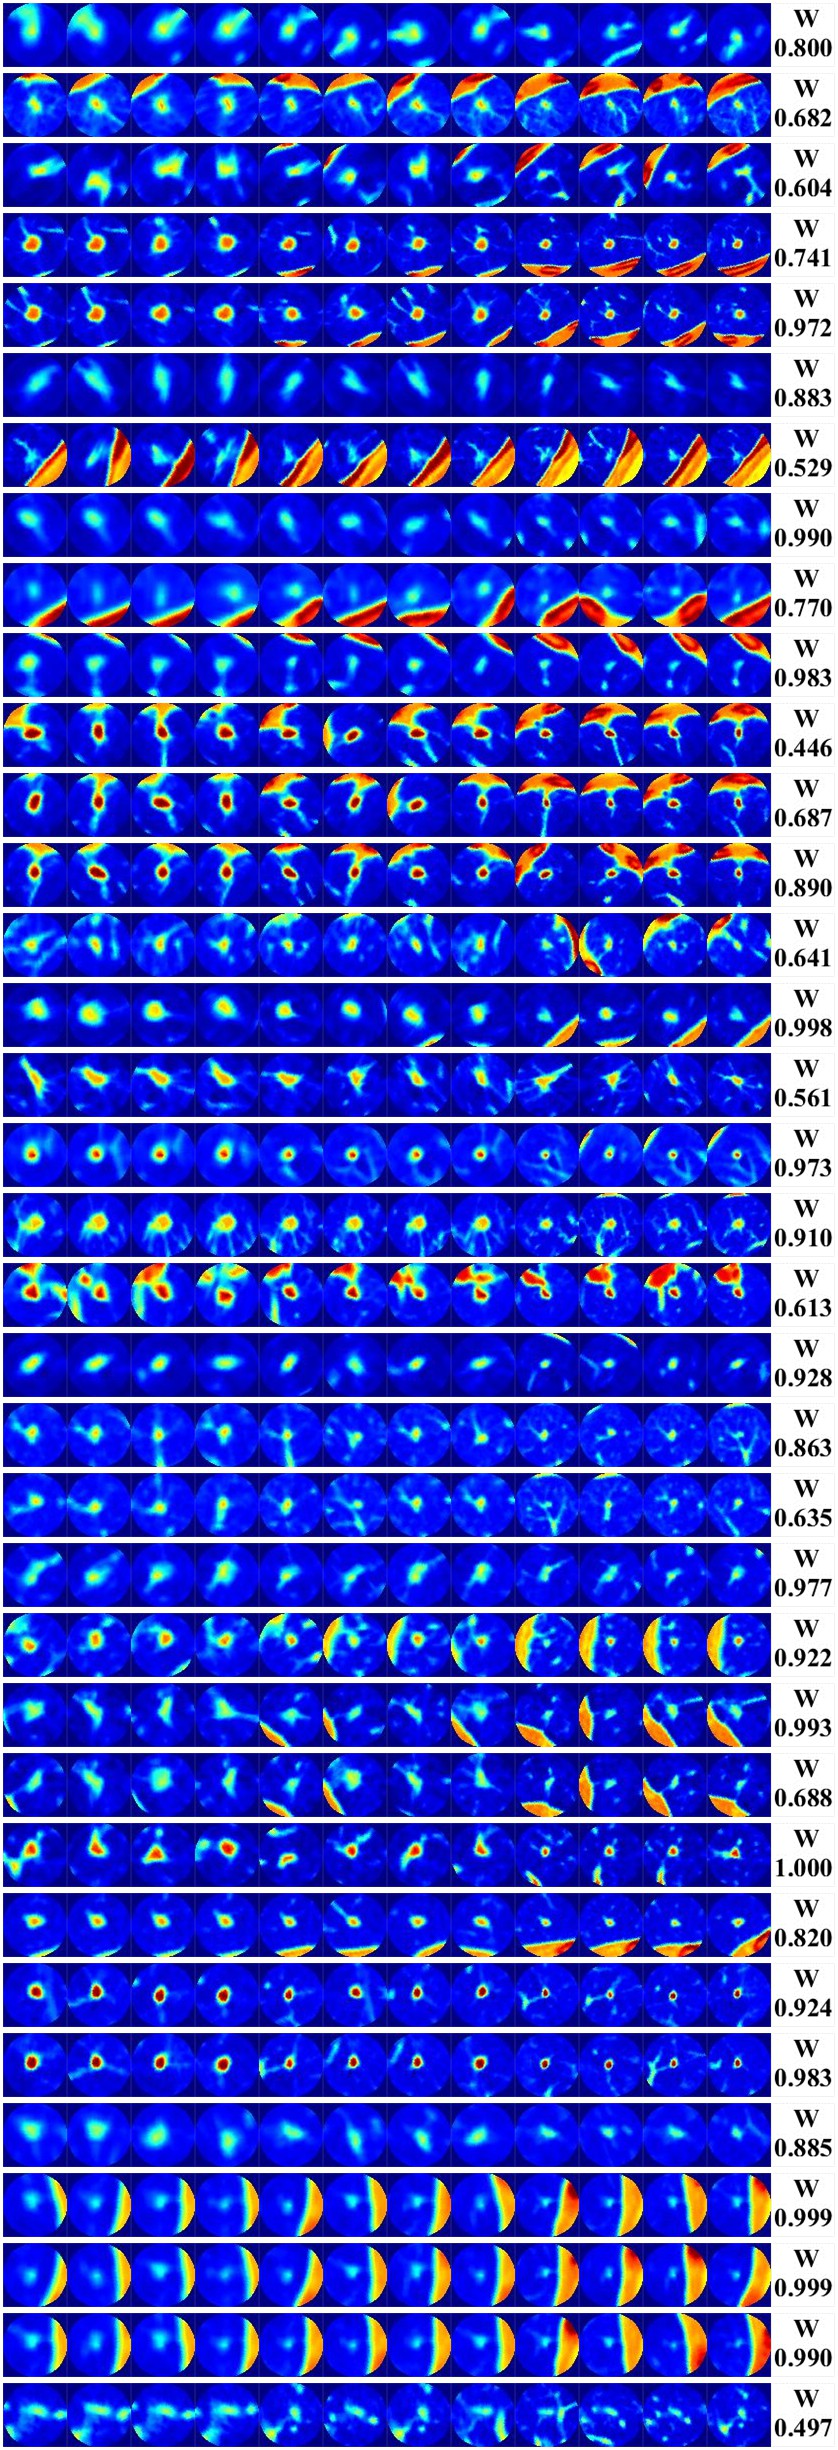
\includegraphics[width=0.45\columnwidth]{./images/lidc-msnodulecircles-iso0}
}
\hspace{.1in}
\subfigure{
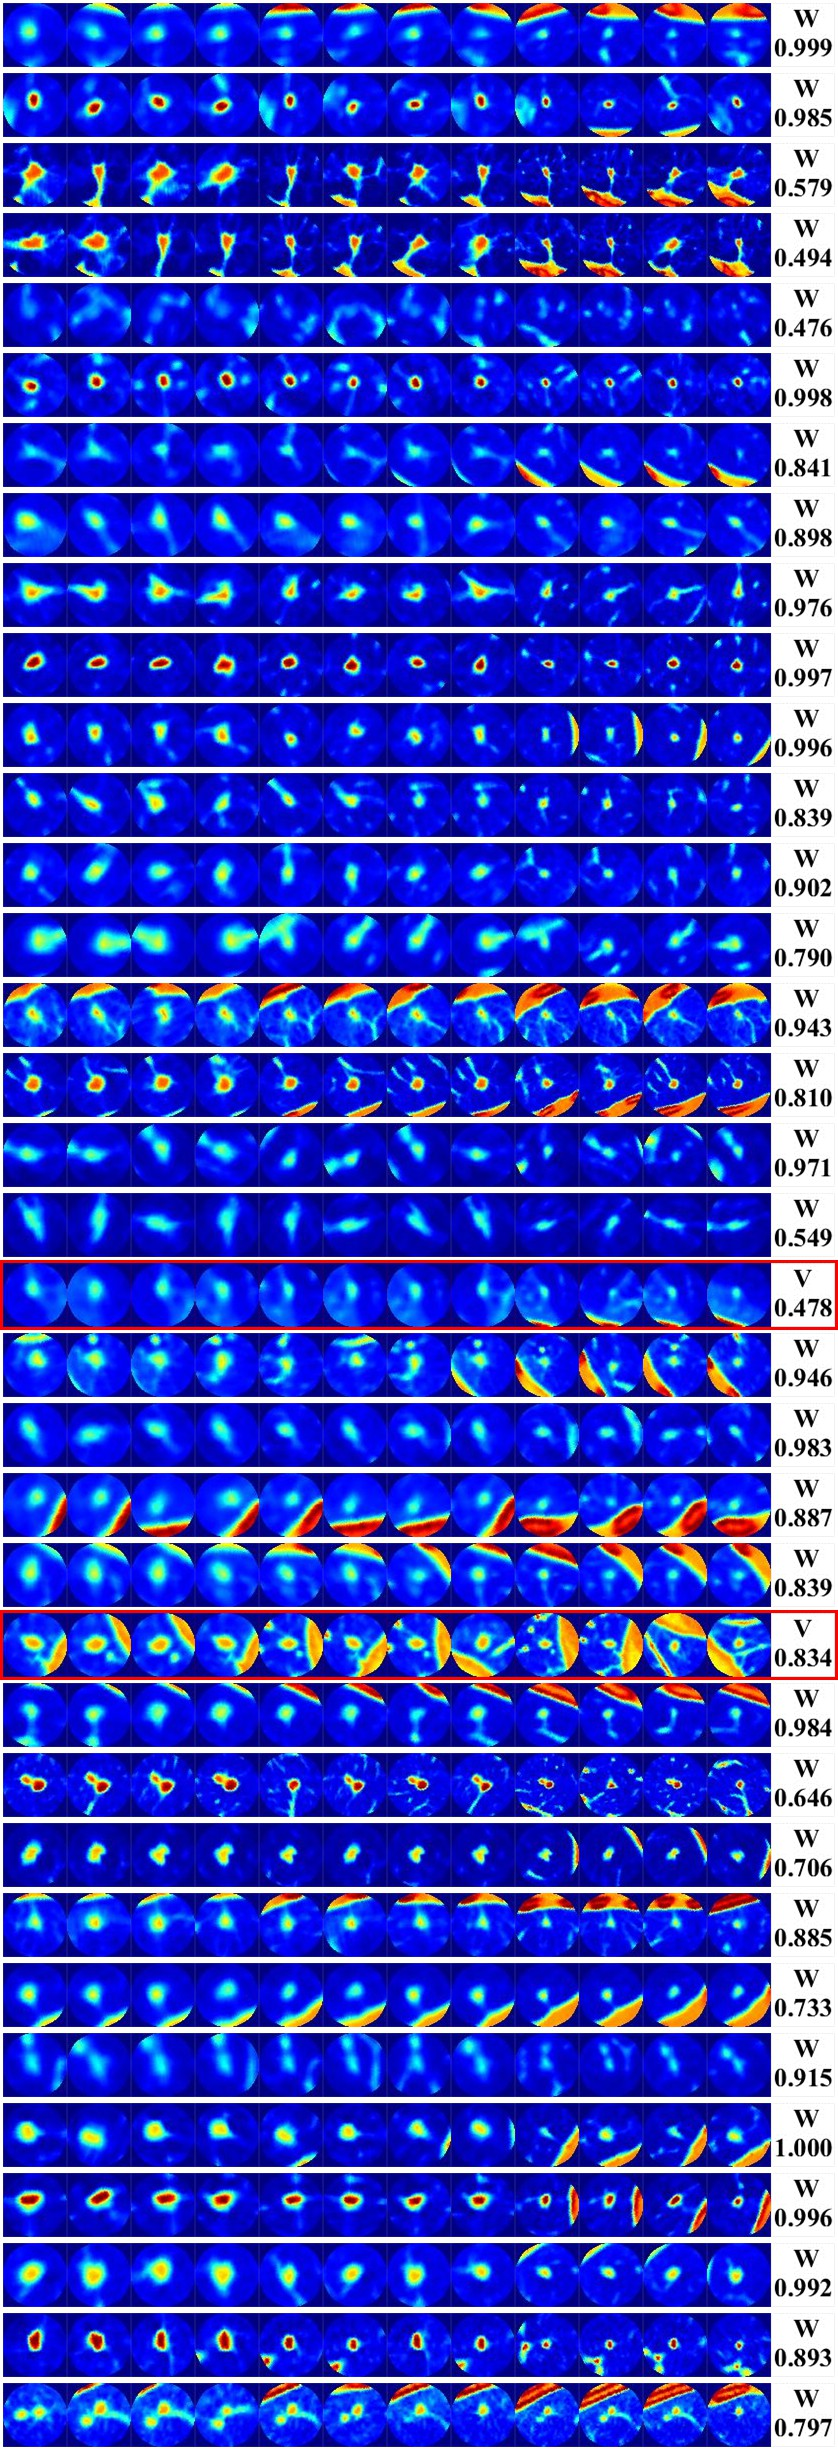
\includegraphics[width=0.45\columnwidth]{./images/lidc-msnodulecircles-iso1}
}
\end{figure}

\newpage
\begin{figure}[H]
\centering
\subfigure{
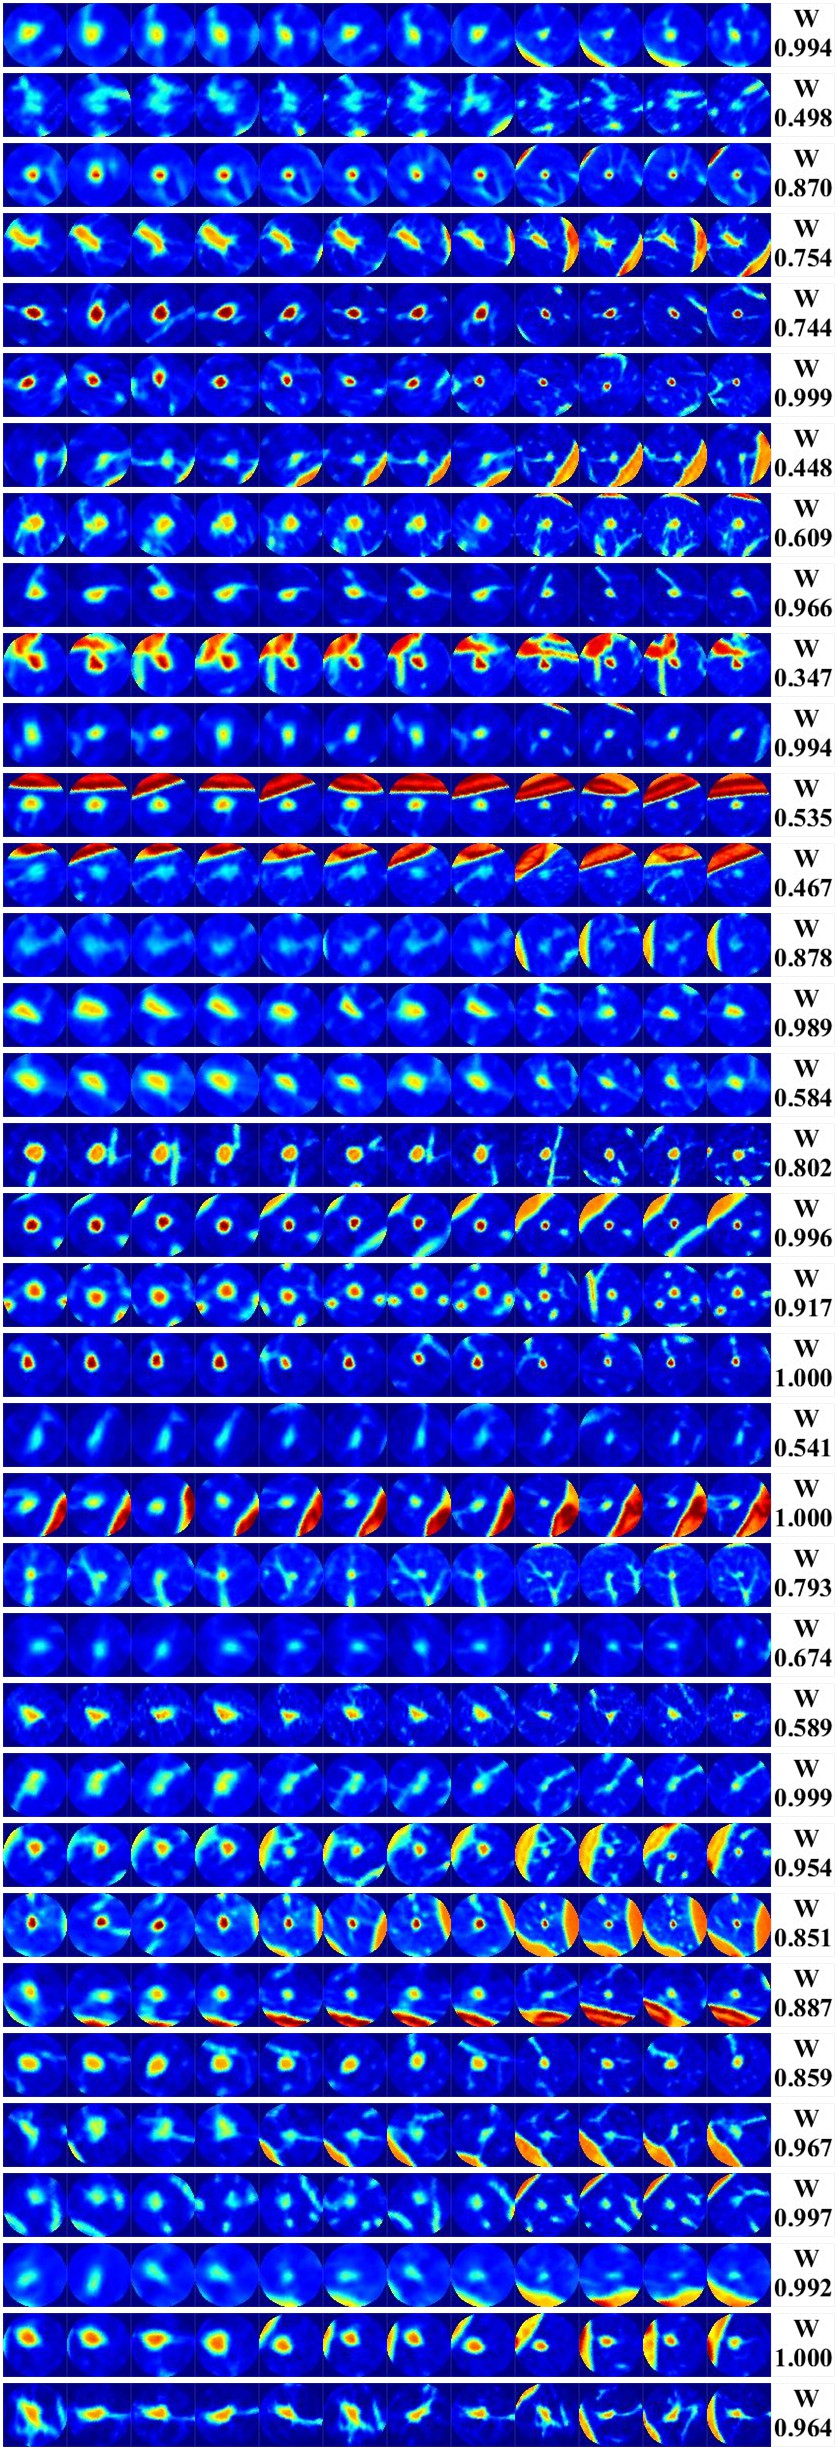
\includegraphics[width=0.45\columnwidth]{./images/lidc-msnodulecircles-iso2}
}
\hspace{.1in}
\subfigure{
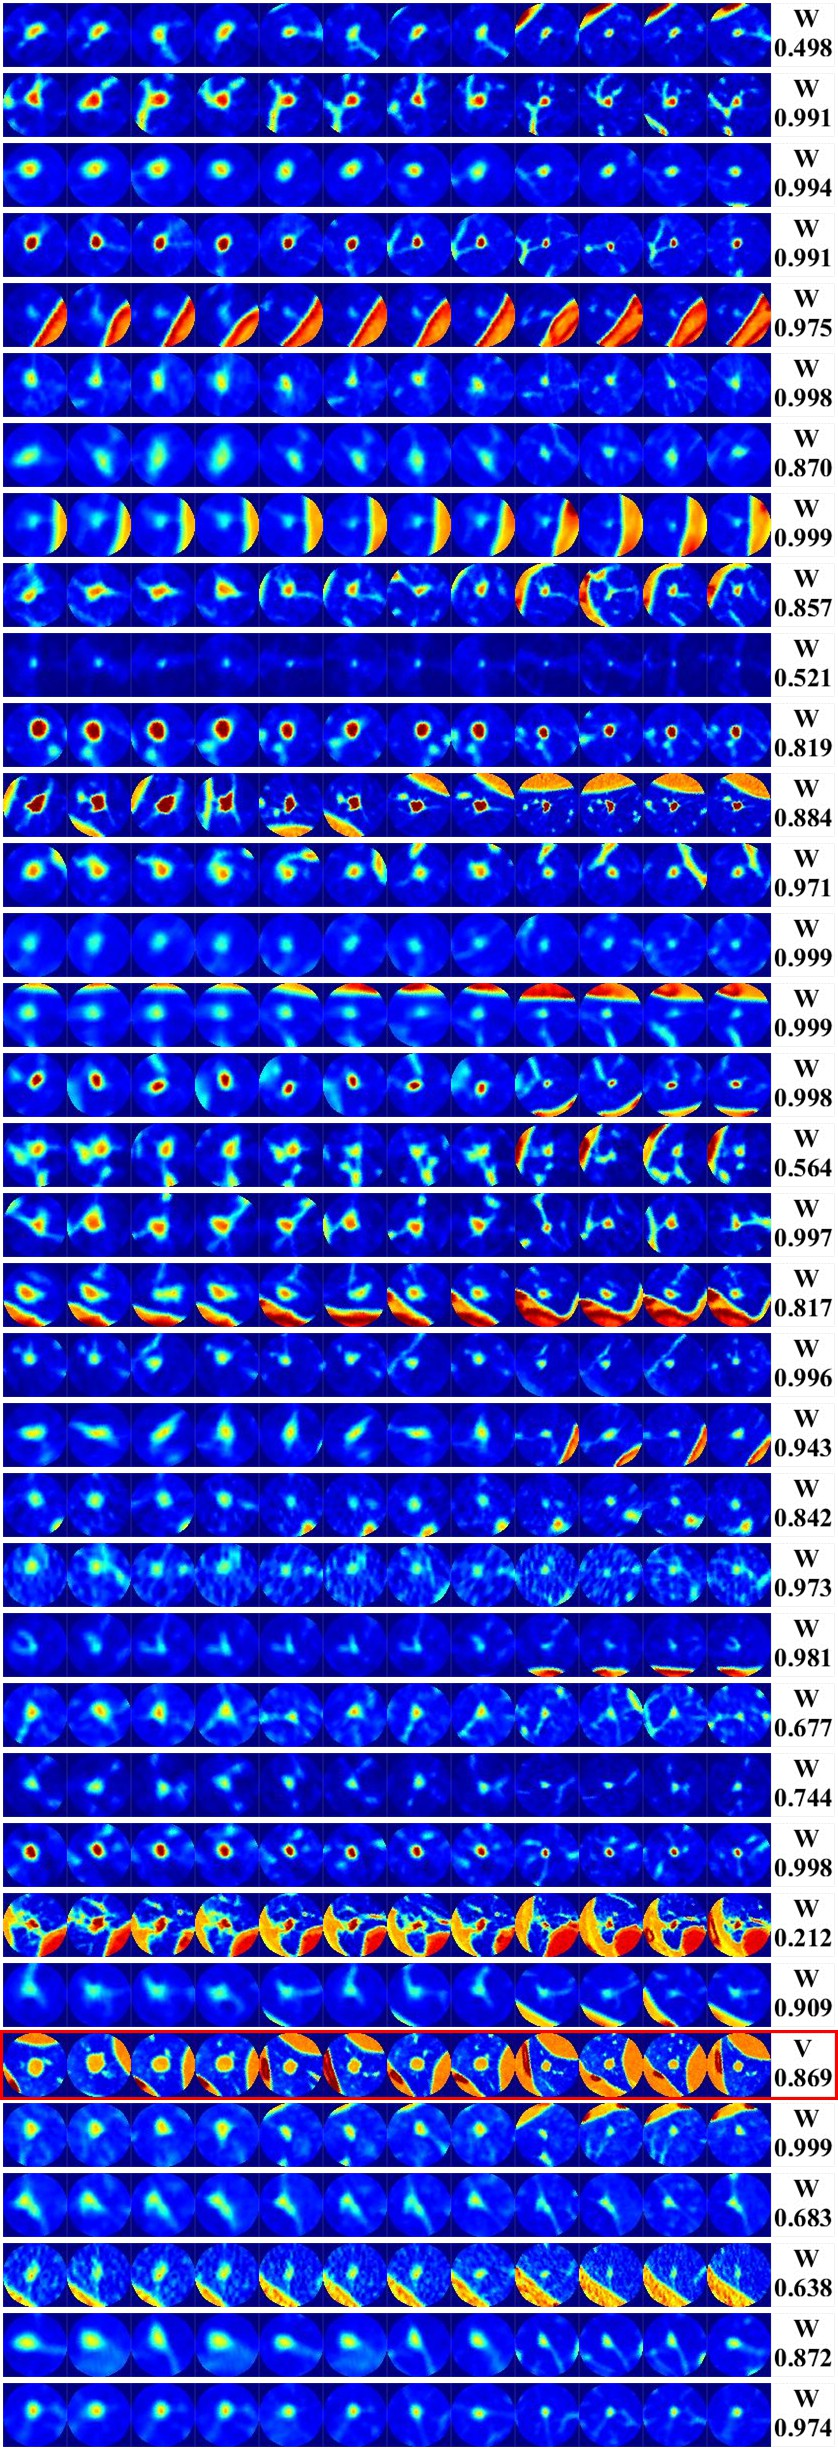
\includegraphics[width=0.45\columnwidth]{./images/lidc-msnodulecircles-iso3}
}
\end{figure}

\newpage
\begin{figure}[H]
 \centering
\subfigure{
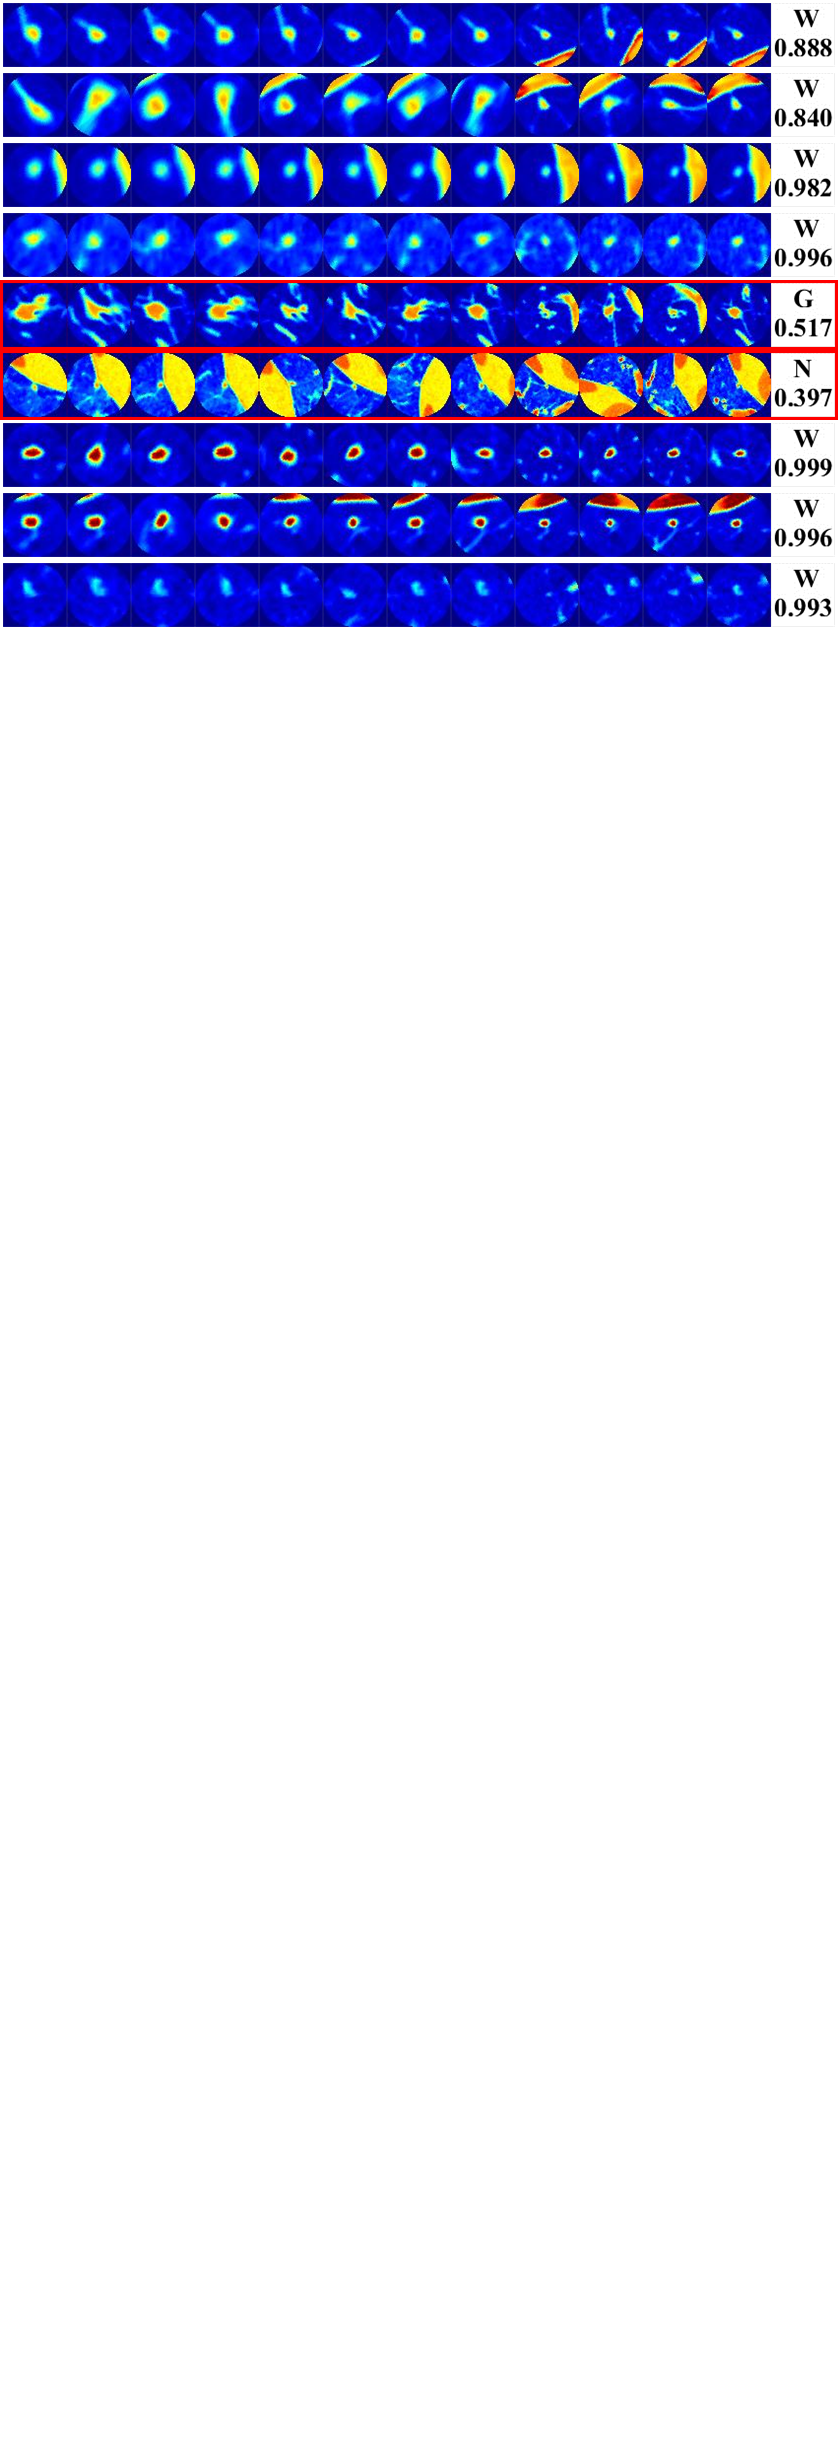
\includegraphics[width=0.45\columnwidth]{./images/lidc-msnodulecircles-iso4}
}
\end{figure}

\newpage
\subsection{GGO for \emph{ms-nodulecircles}}
\begin{figure}[H]
\centering
\subfigure{
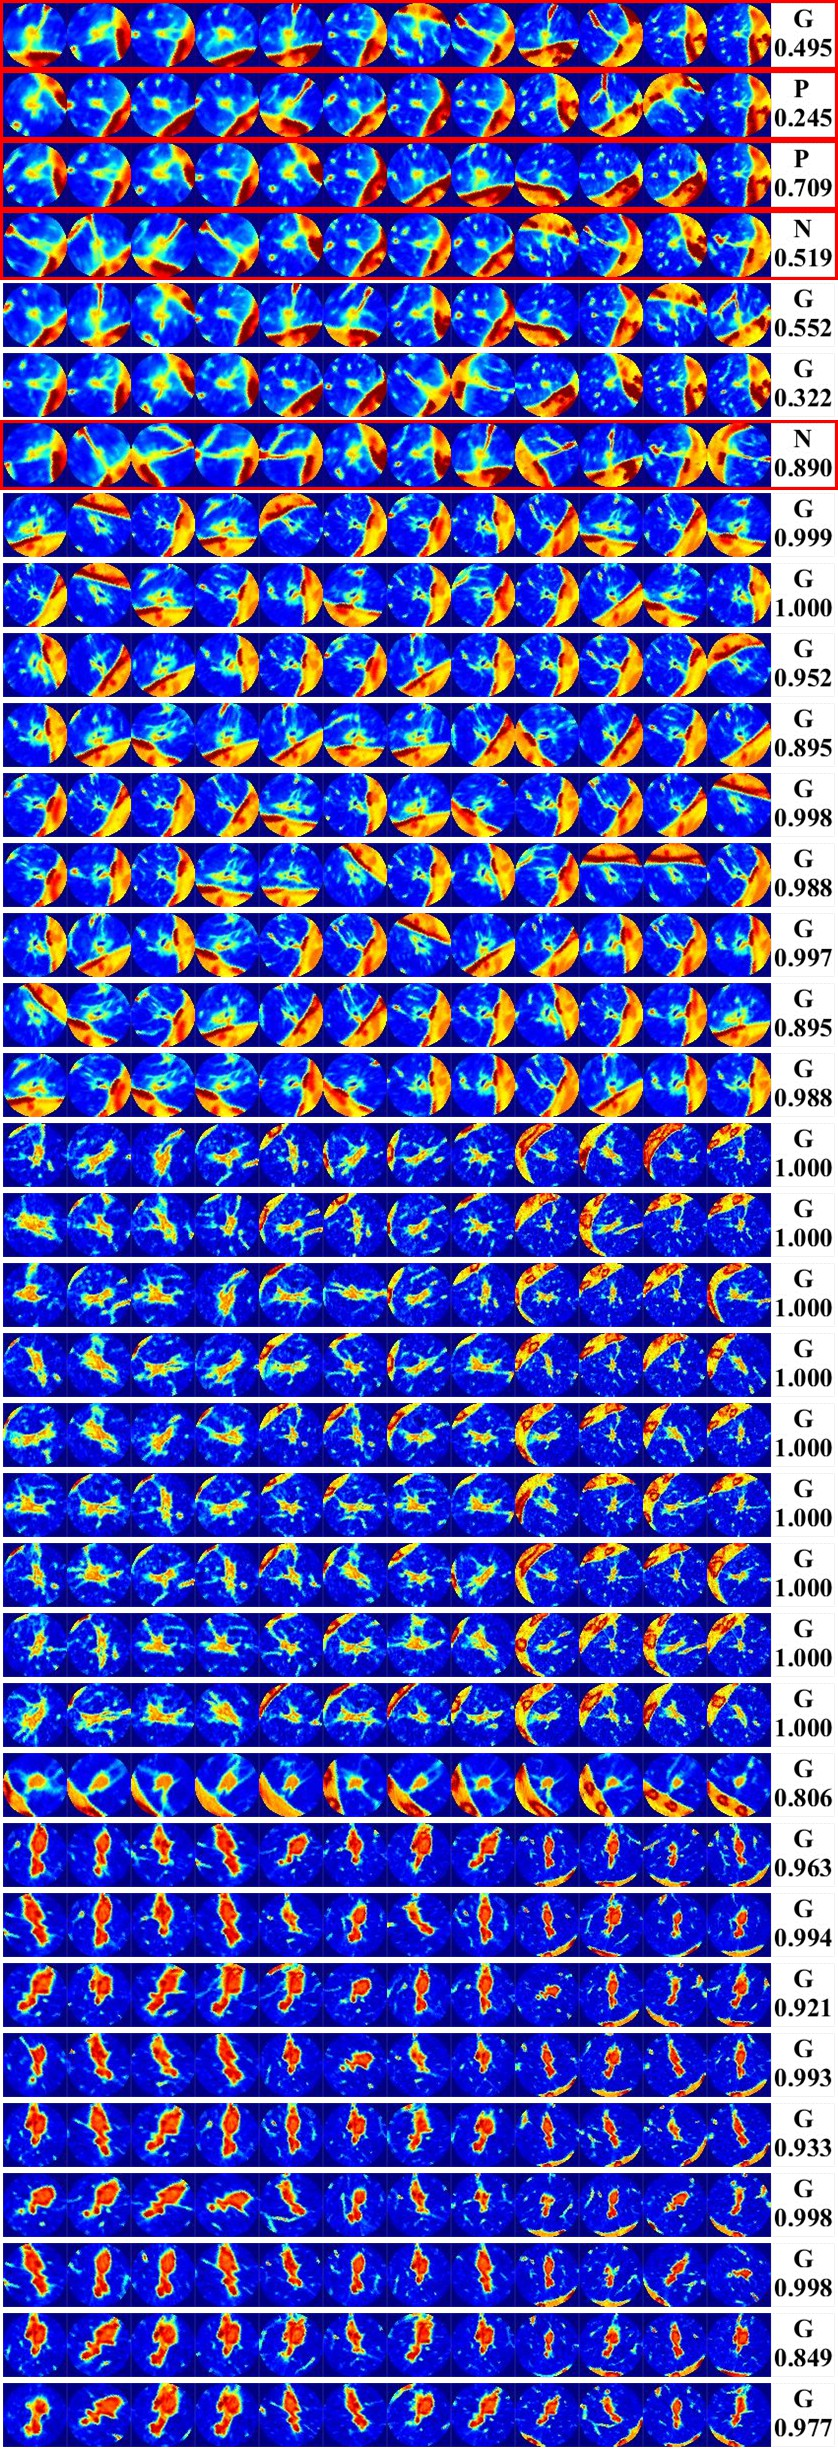
\includegraphics[width=0.45\columnwidth]{./images/lidc-msnodulecircles-ggo0}
}
\hspace{.1in}
\subfigure{
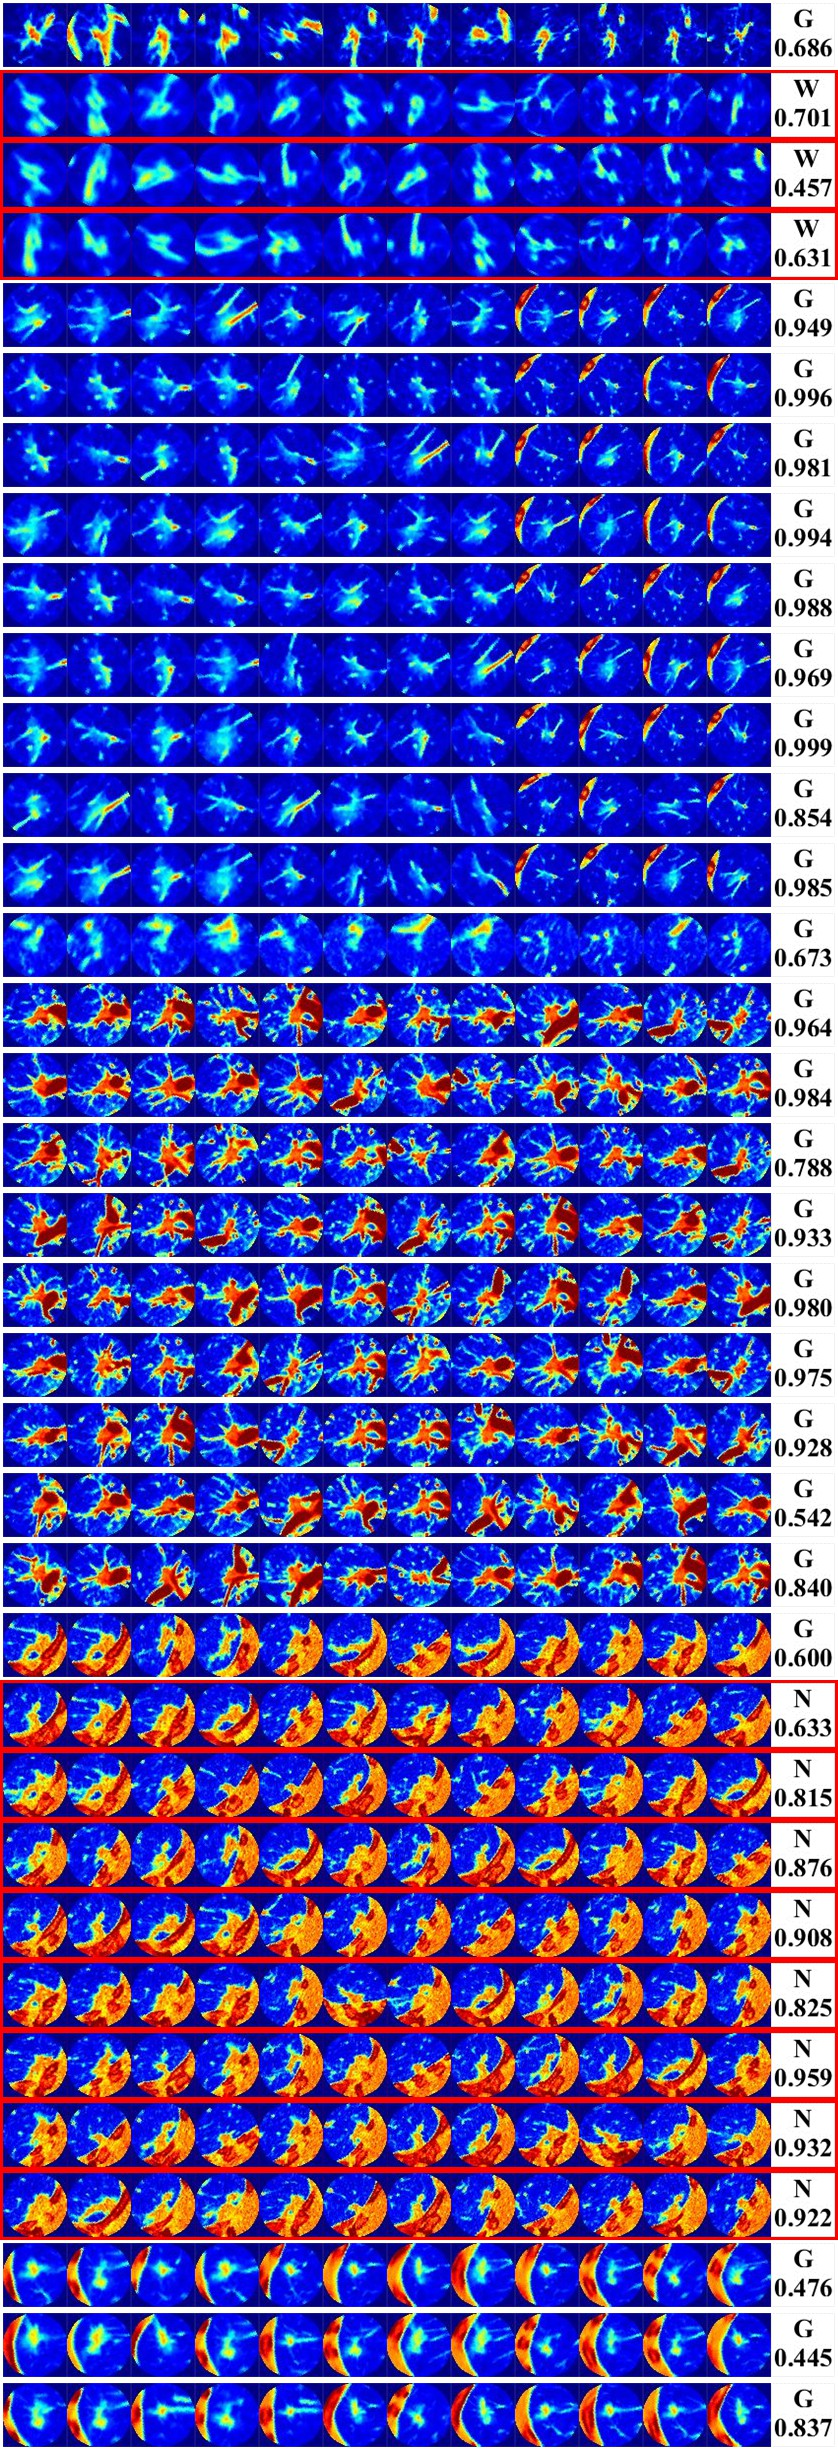
\includegraphics[width=0.45\columnwidth]{./images/lidc-msnodulecircles-ggo1}
}
\end{figure}
\newpage
\begin{figure}[H]
\centering
\subfigure{
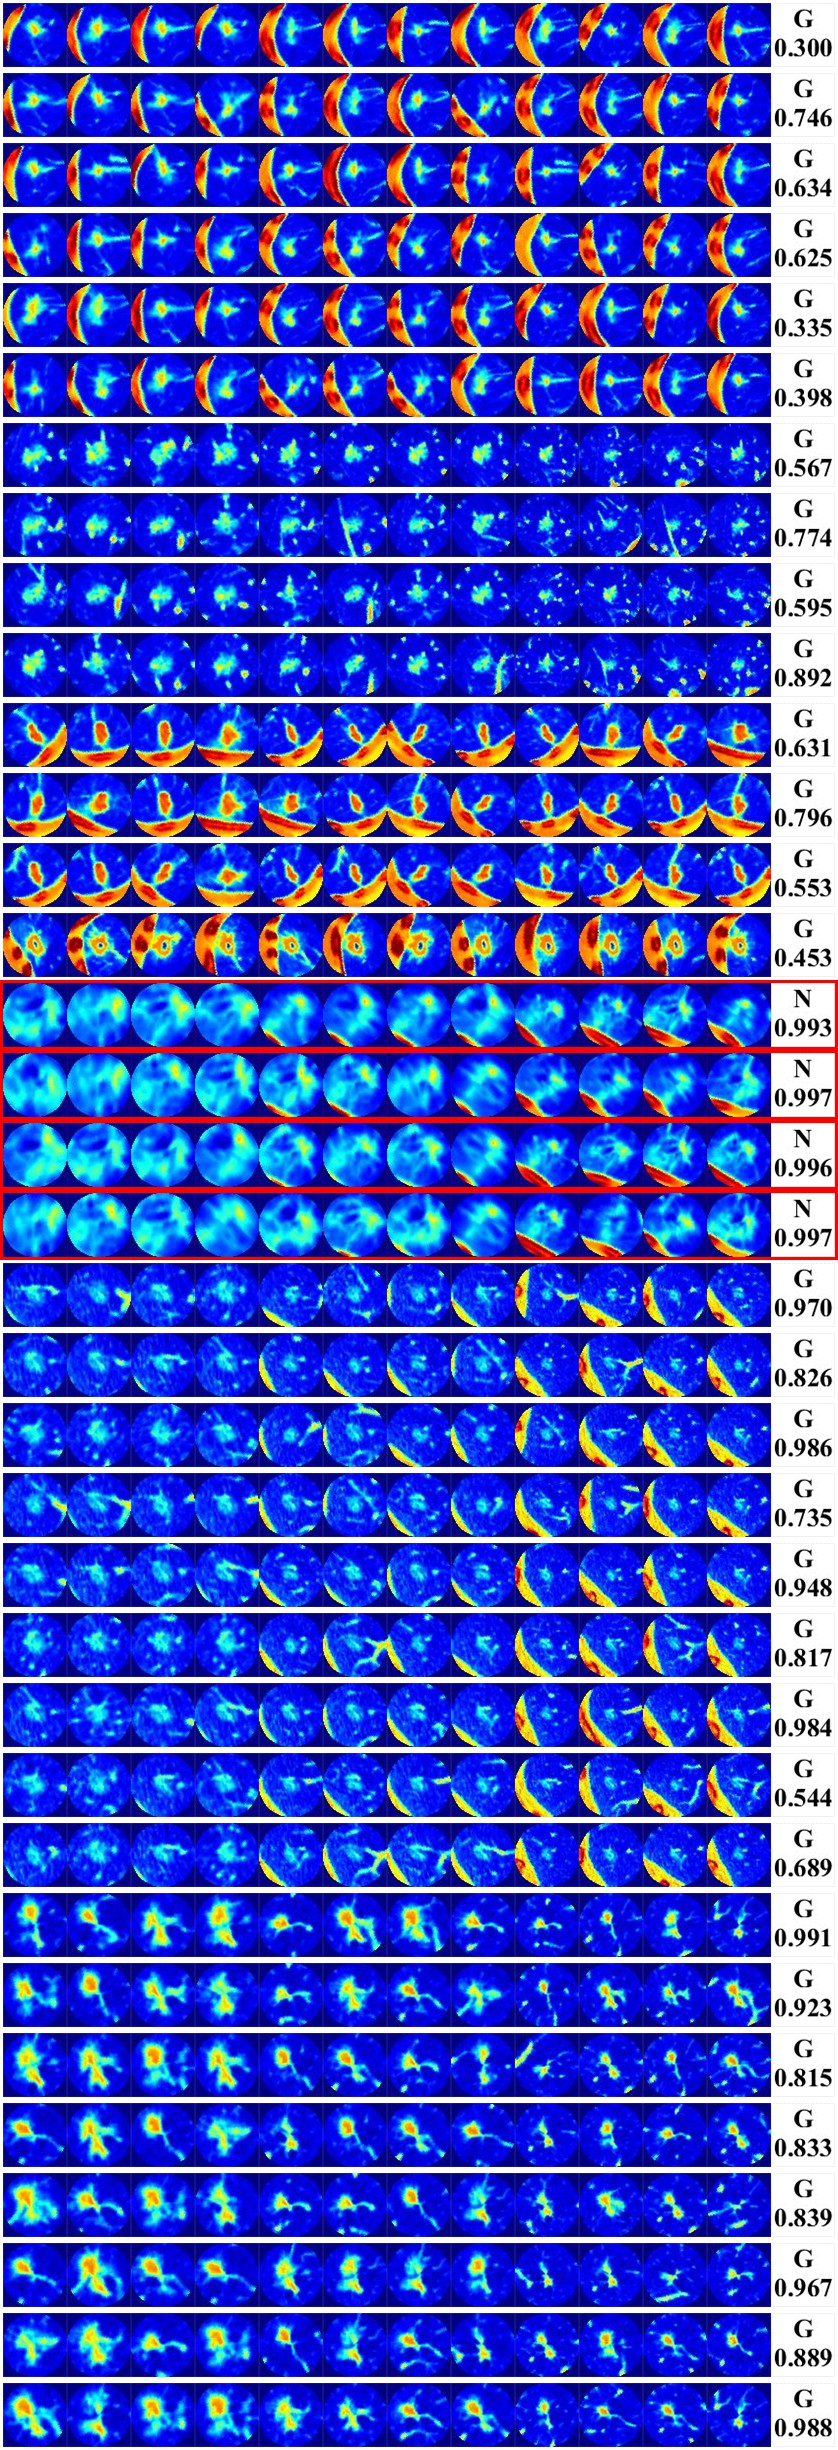
\includegraphics[width=0.45\columnwidth]{./images/lidc-msnodulecircles-ggo2}
}
\hspace{.1in}
\subfigure{
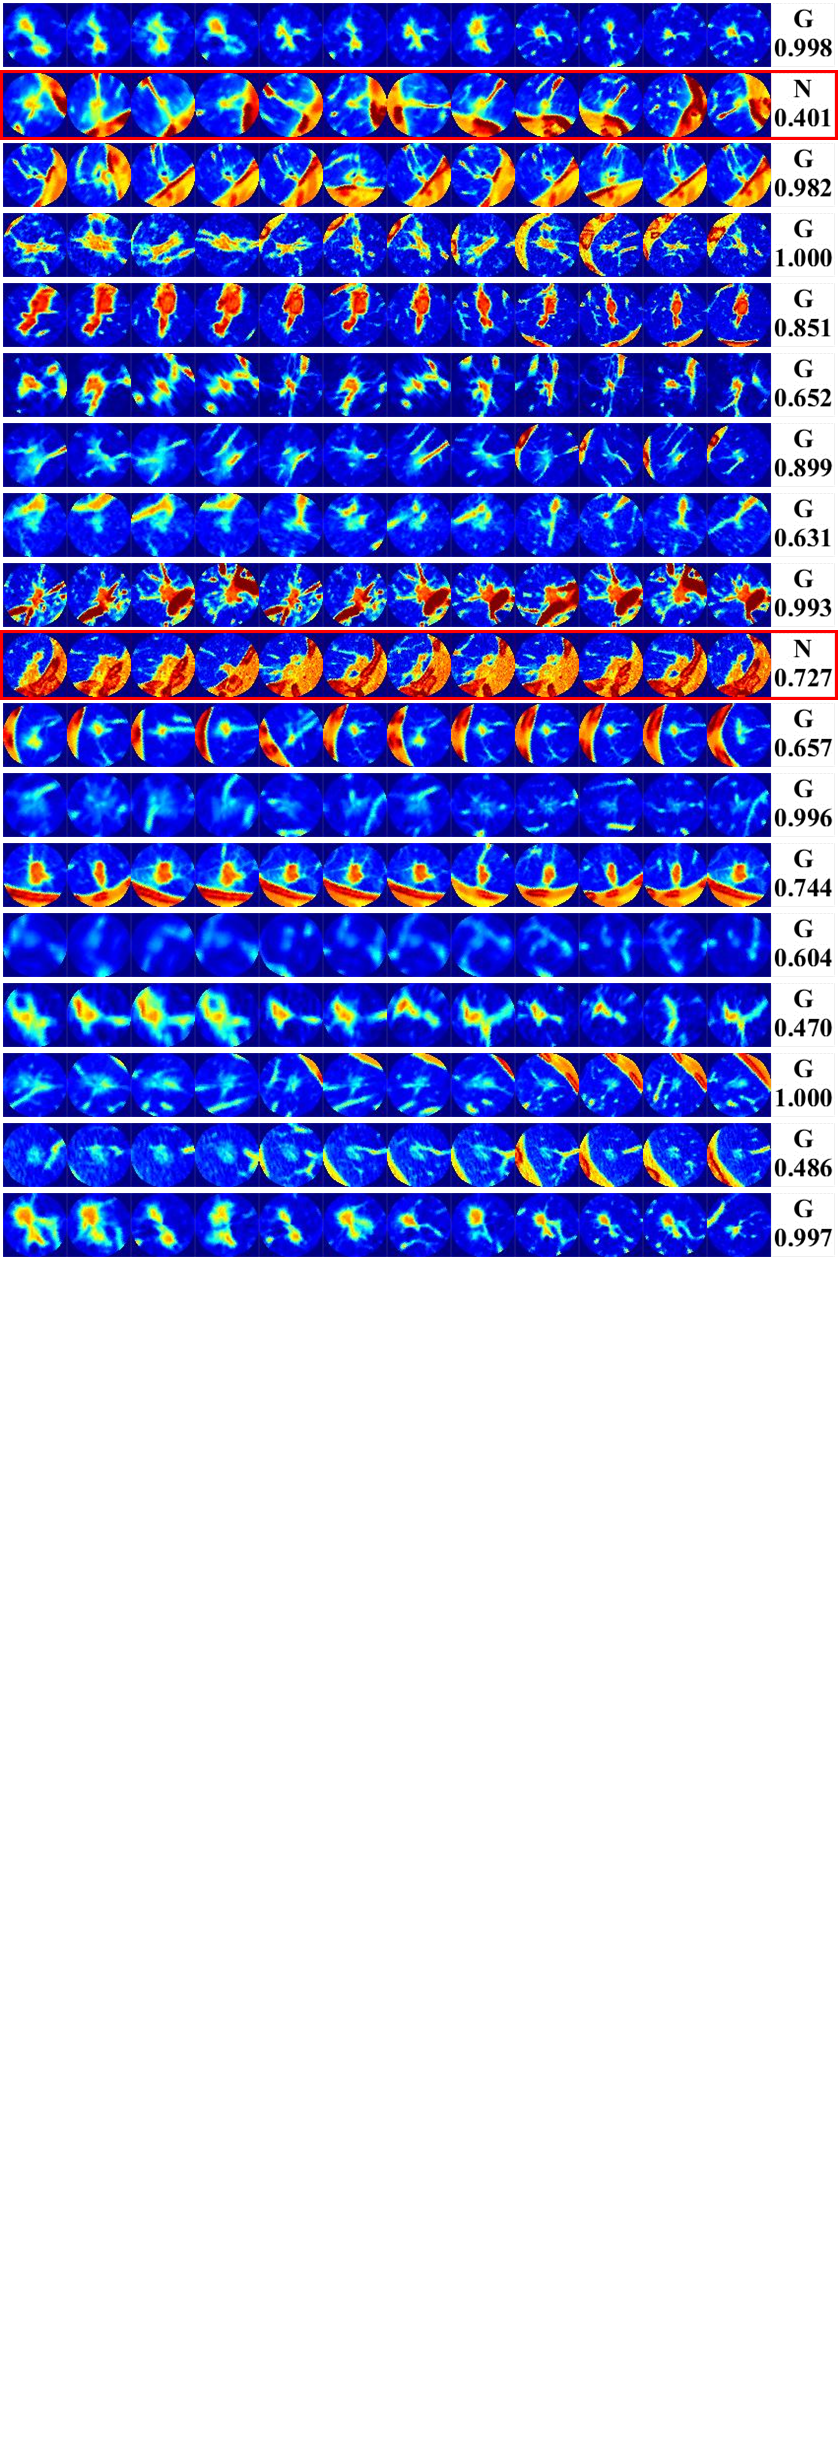
\includegraphics[width=0.45\columnwidth]{./images/lidc-msnodulecircles-ggo3}
}
\end{figure}



\newpage
\subsection{Juxta-pleural for \emph{ms-nodulecircles}}
\begin{figure}[H]
\centering
\subfigure{
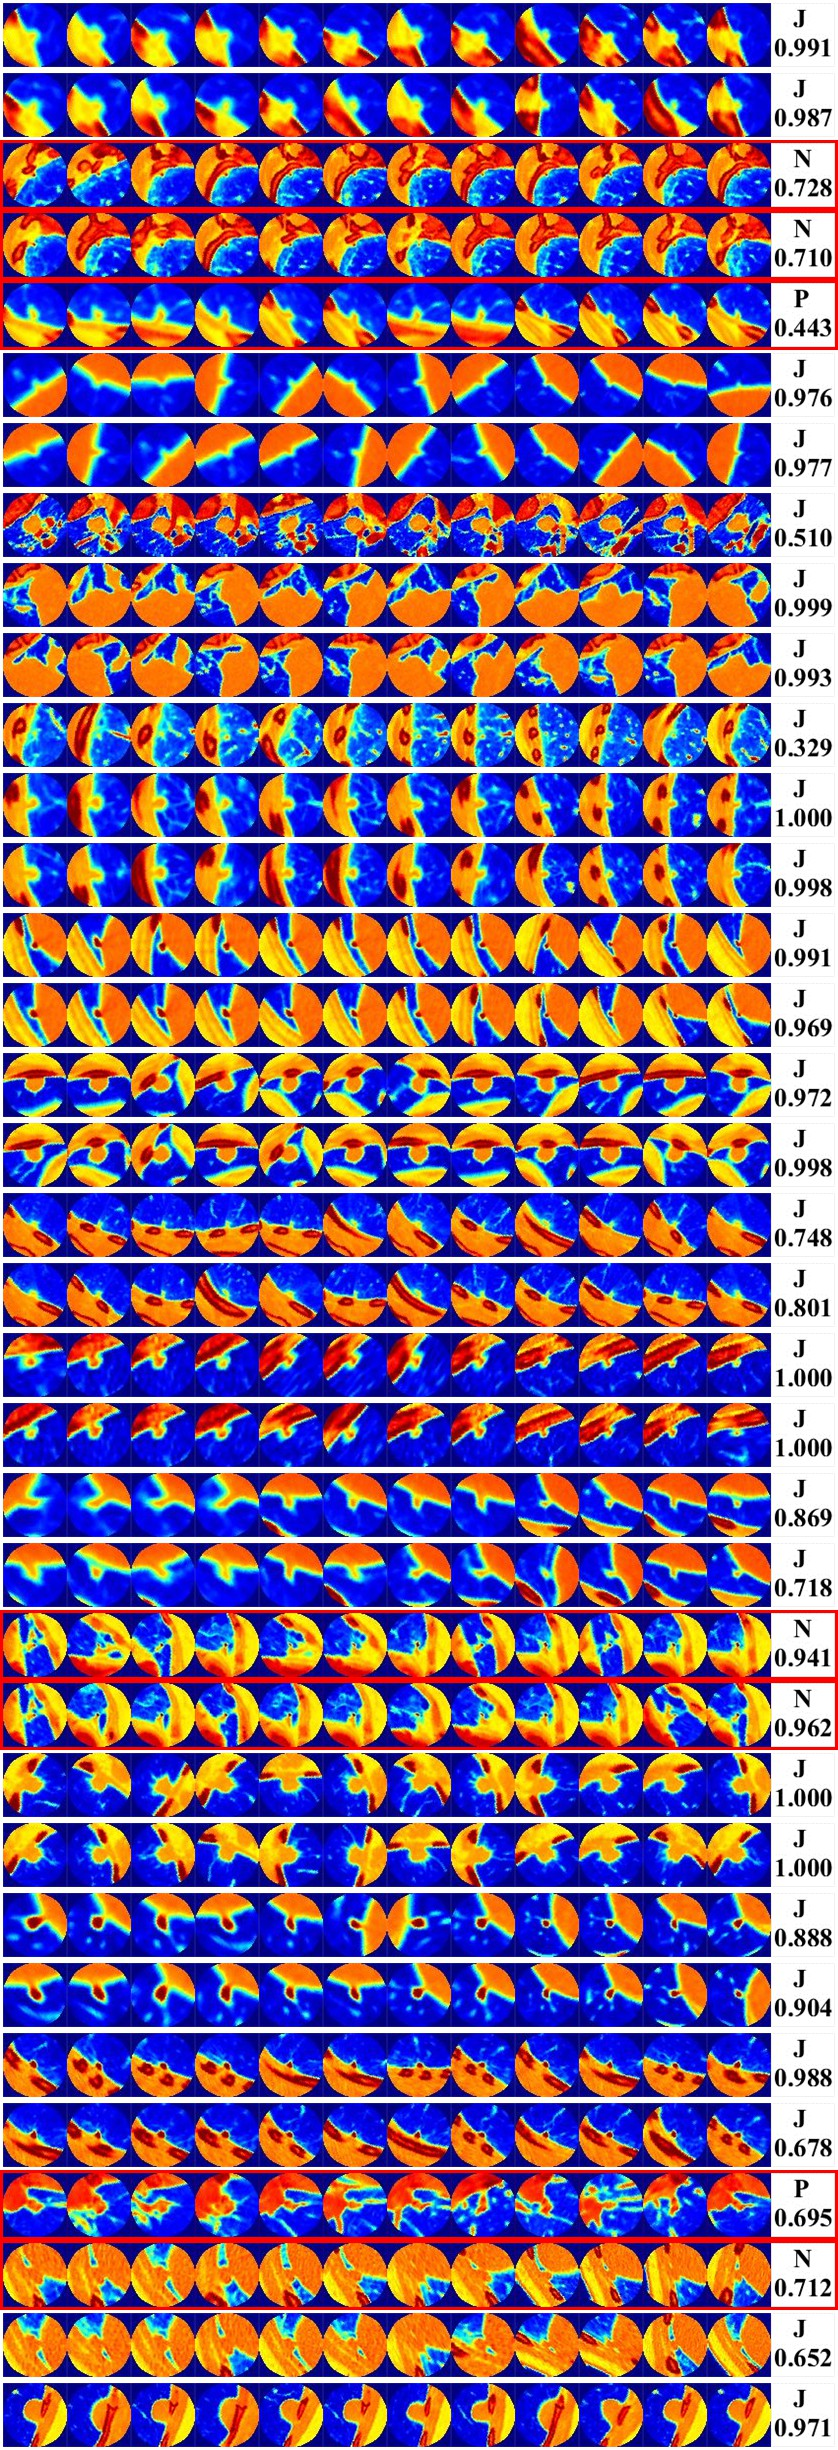
\includegraphics[width=0.45\columnwidth]{./images/lidc-msnodulecircles-wall0}
}
\hspace{.1in}
\subfigure{
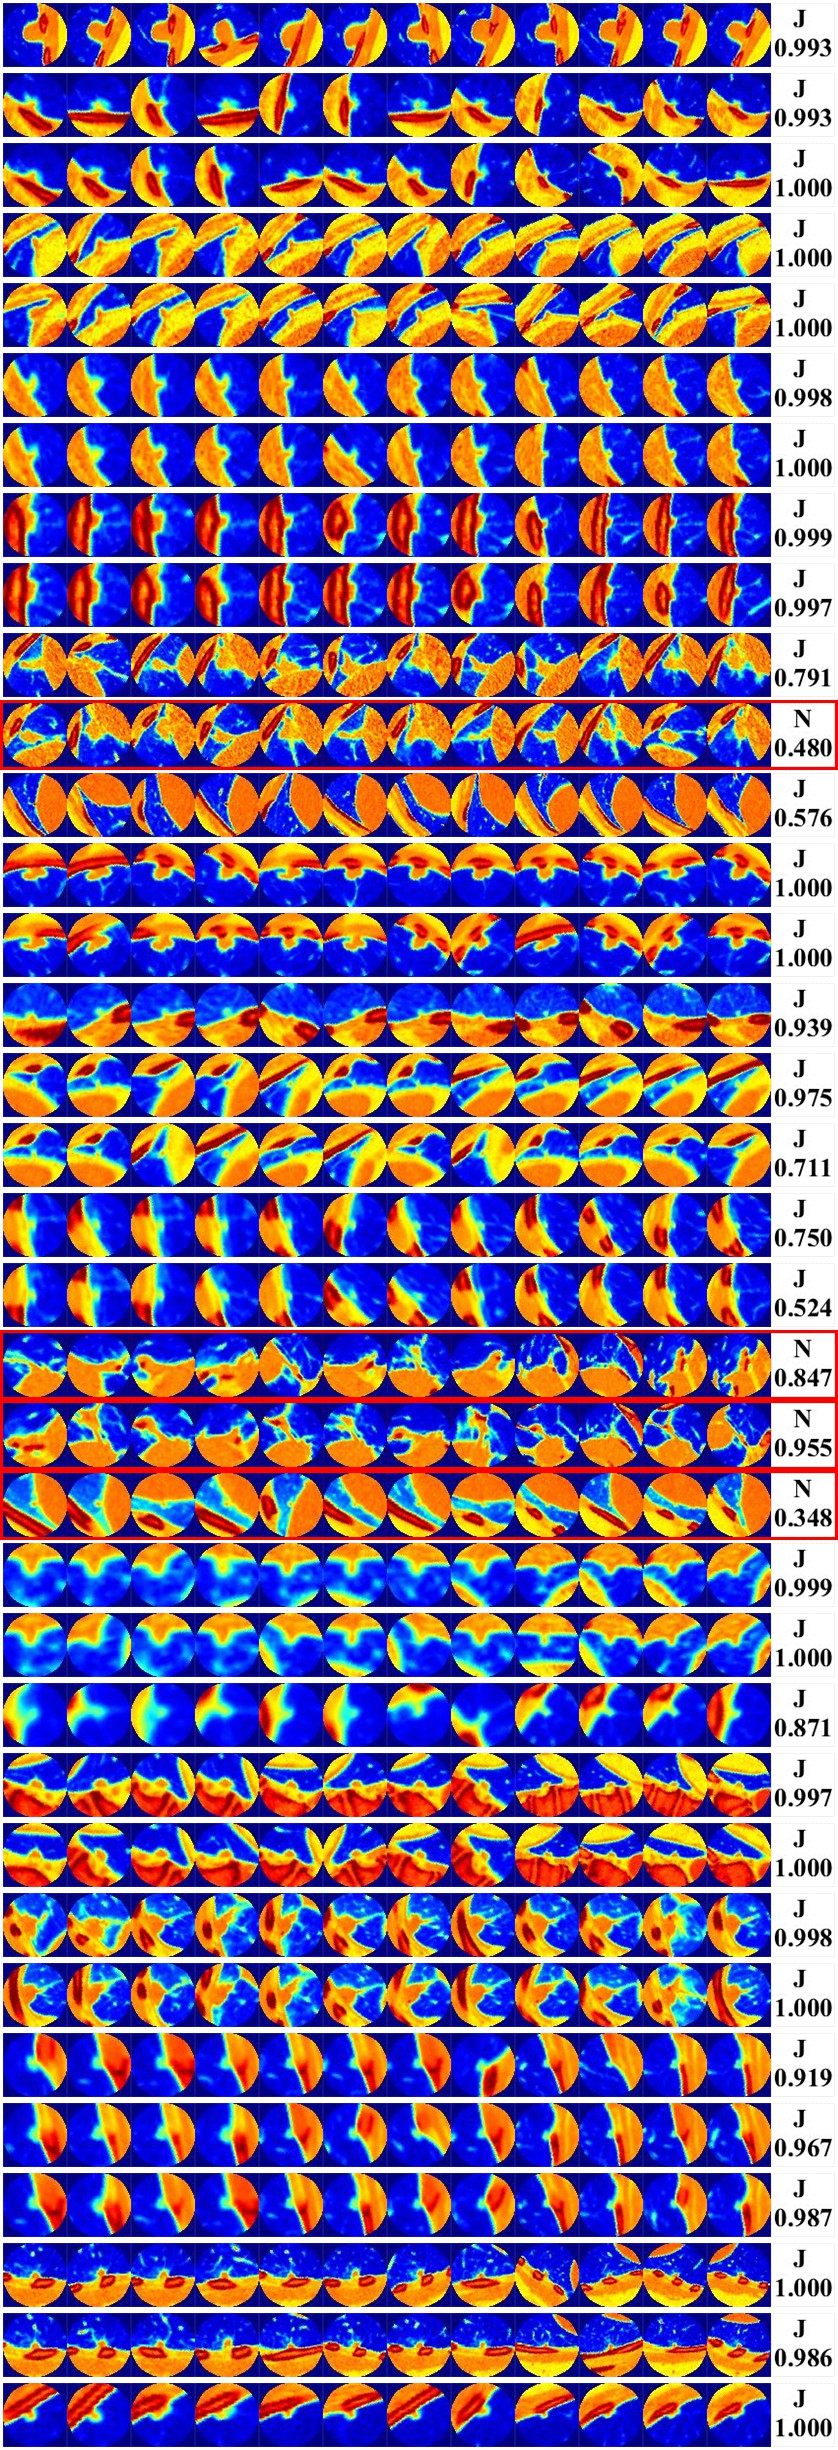
\includegraphics[width=0.45\columnwidth]{./images/lidc-msnodulecircles-wall1}
}
\end{figure}
\newpage
\begin{figure}[H]
\centering
\subfigure{
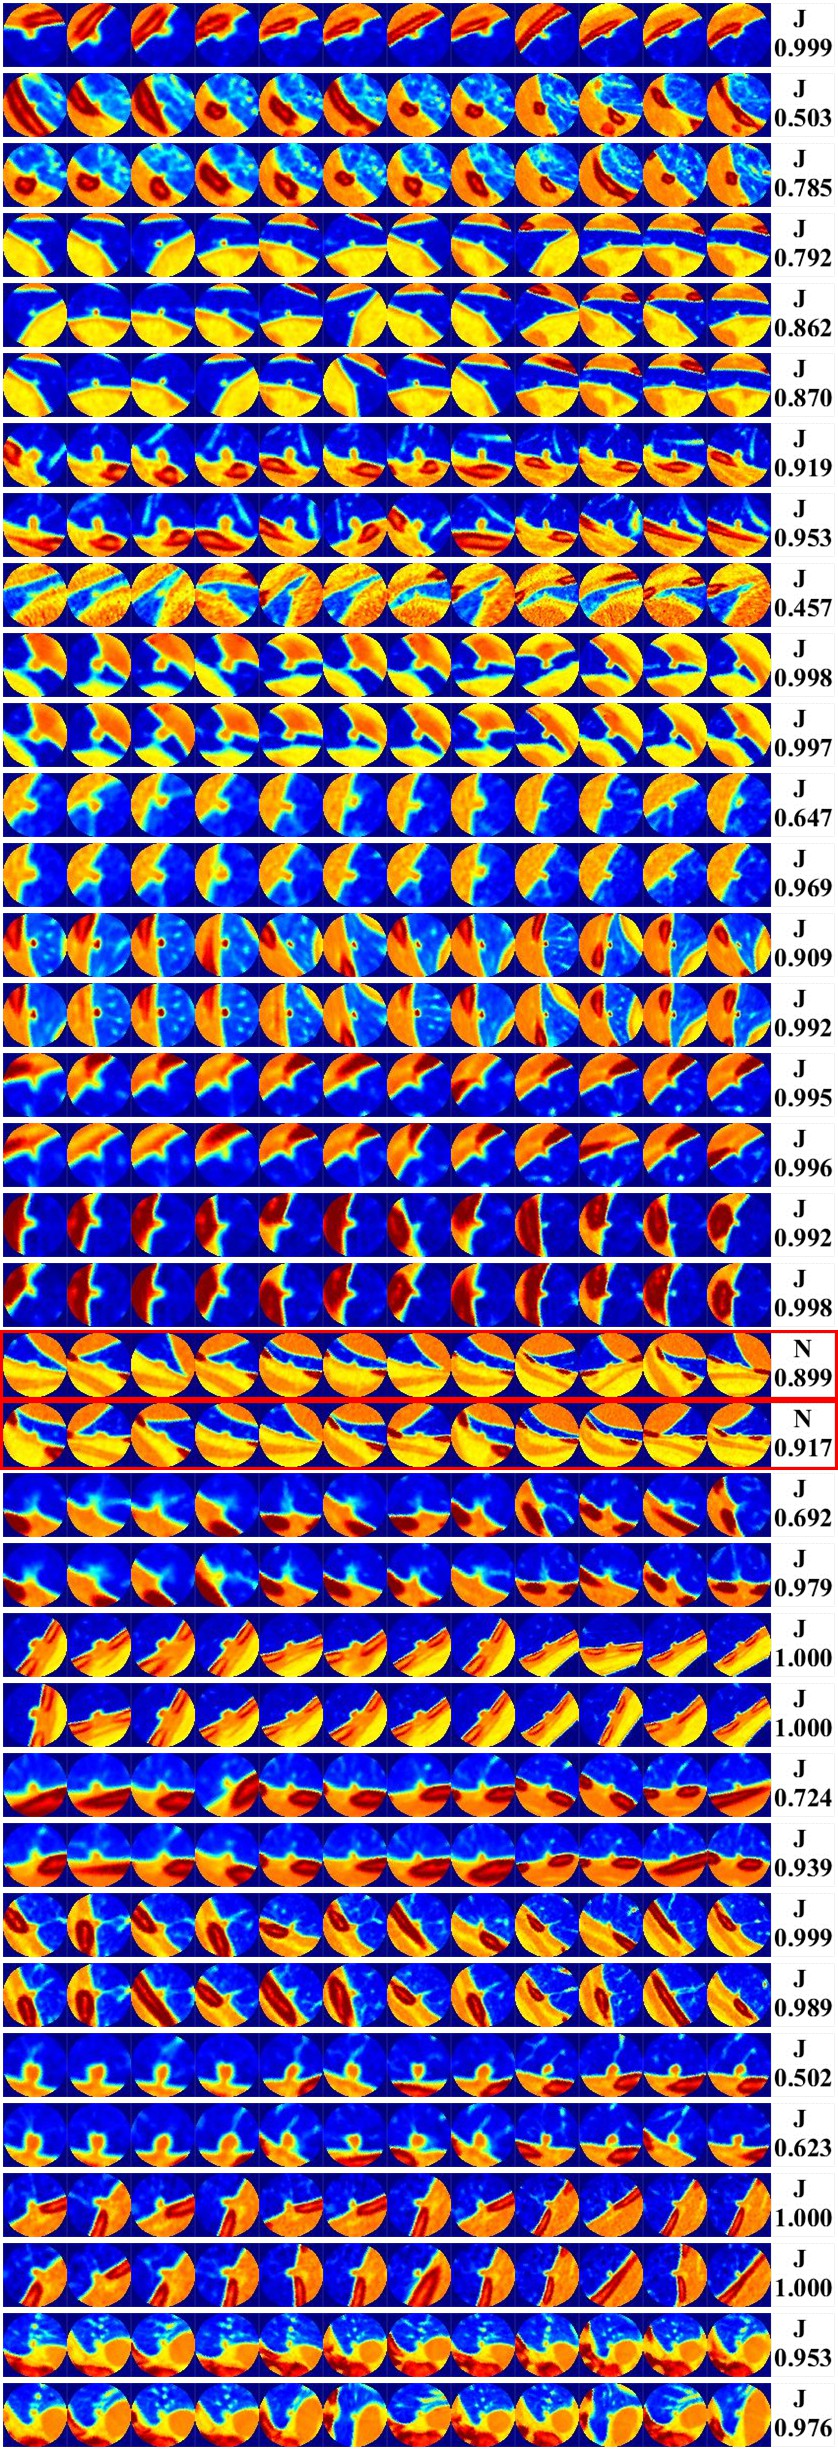
\includegraphics[width=0.45\columnwidth]{./images/lidc-msnodulecircles-wall2}
}
\hspace{.1in}
\subfigure{
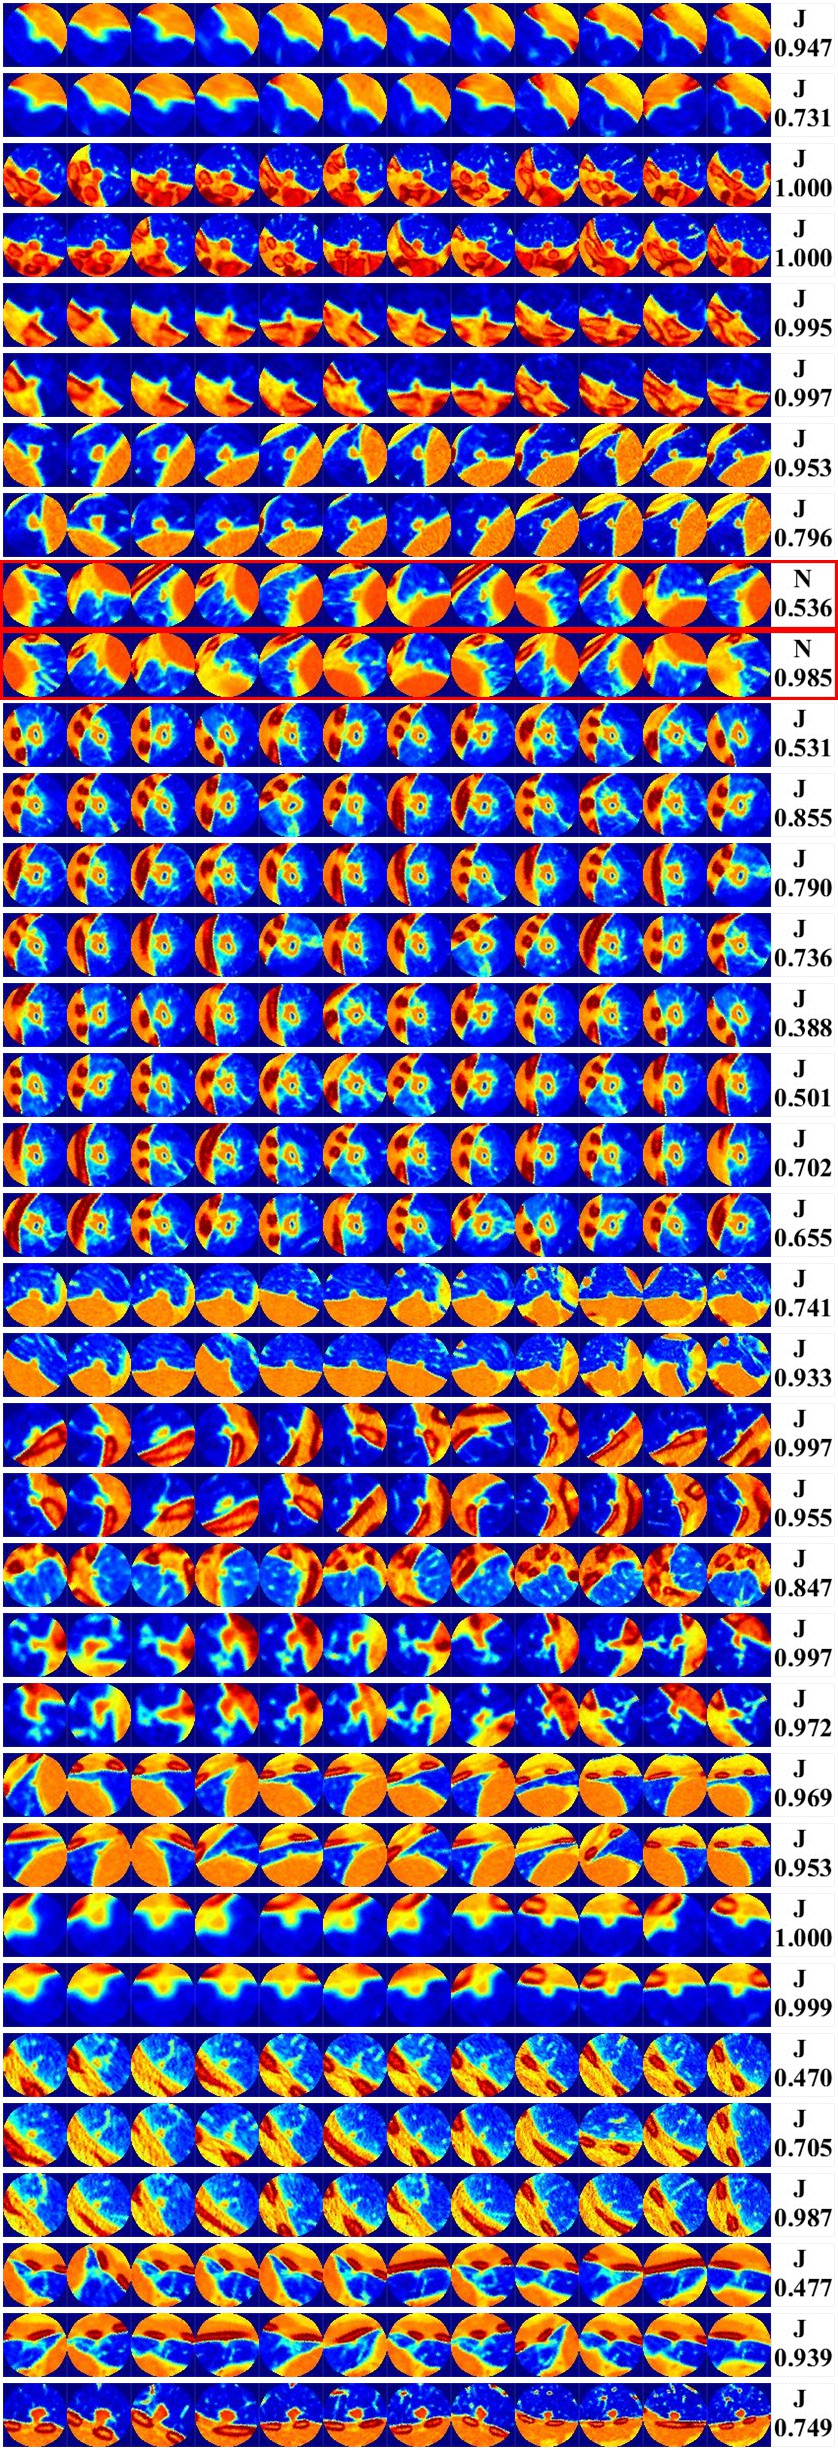
\includegraphics[width=0.45\columnwidth]{./images/lidc-msnodulecircles-wall3}
}
\end{figure}
\newpage
\begin{figure}[H]
\centering
\subfigure{
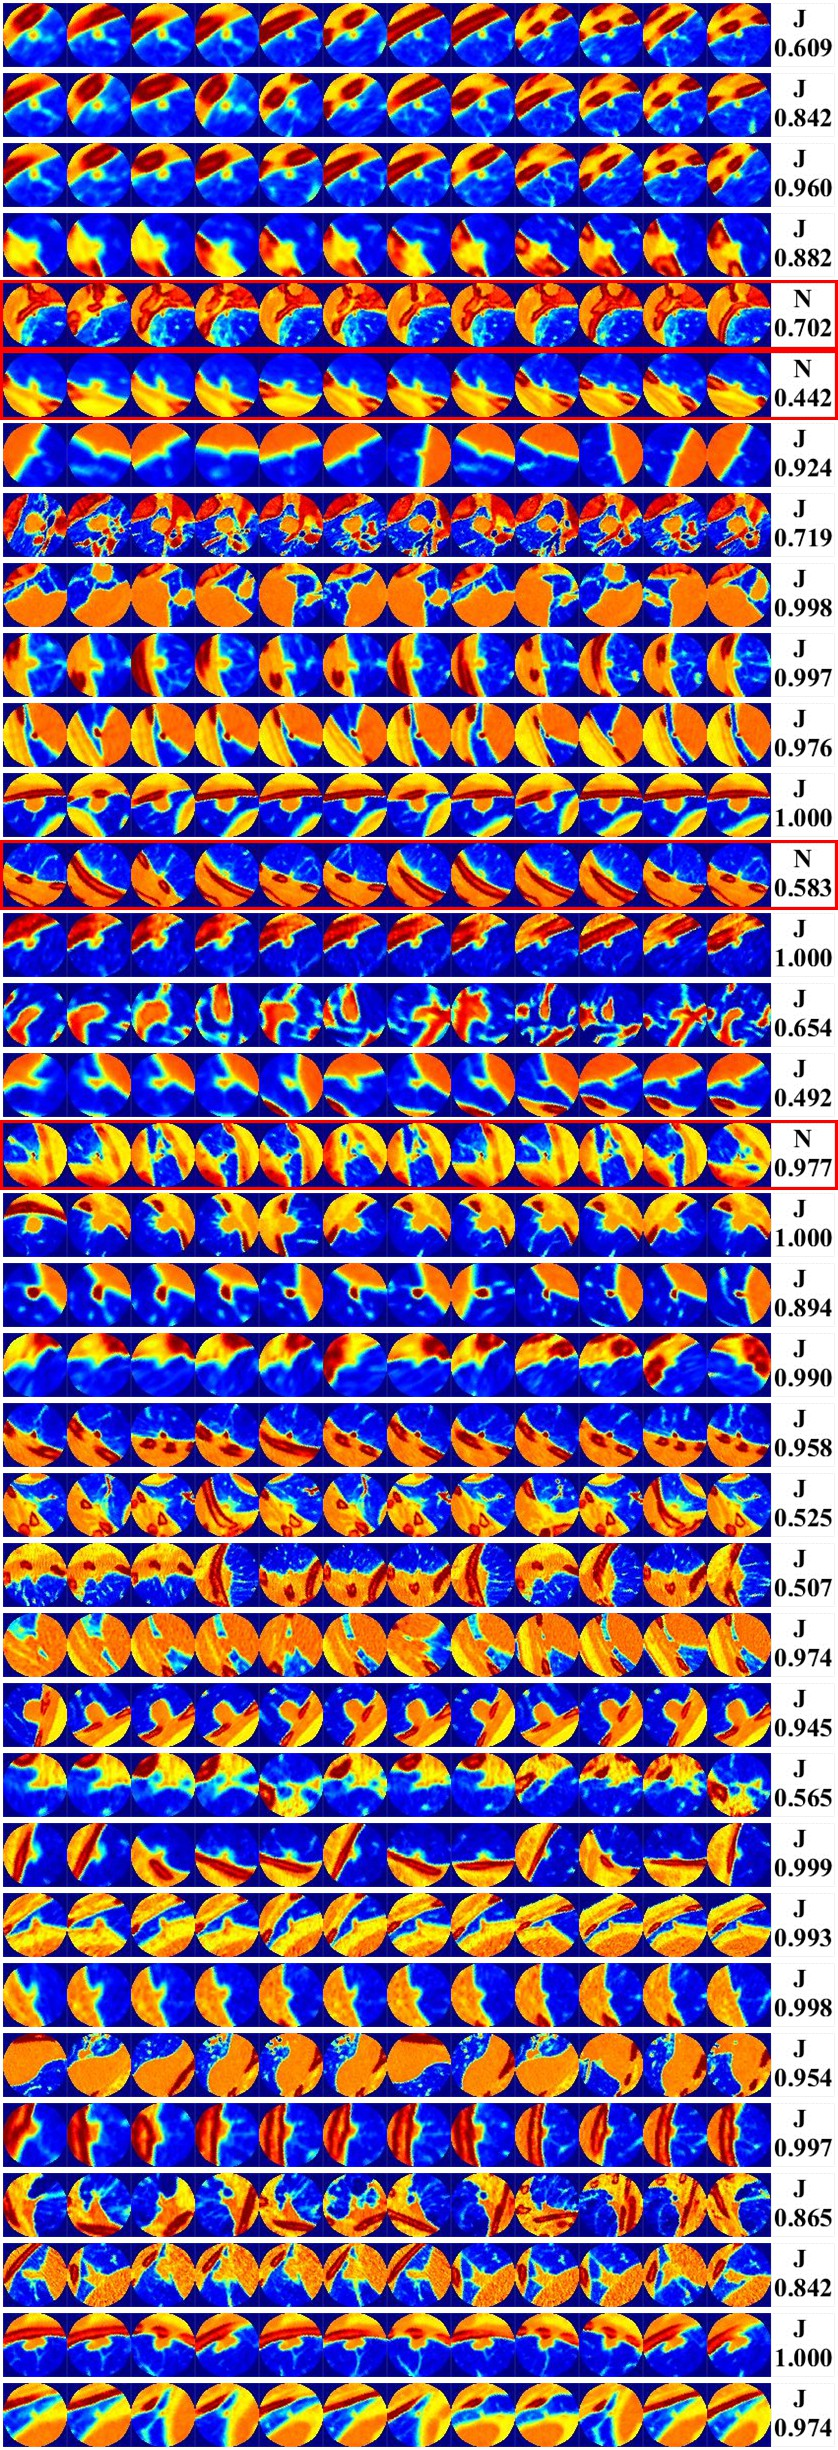
\includegraphics[width=0.45\columnwidth]{./images/lidc-msnodulecircles-wall4}
}
\hspace{.1in}
\subfigure{
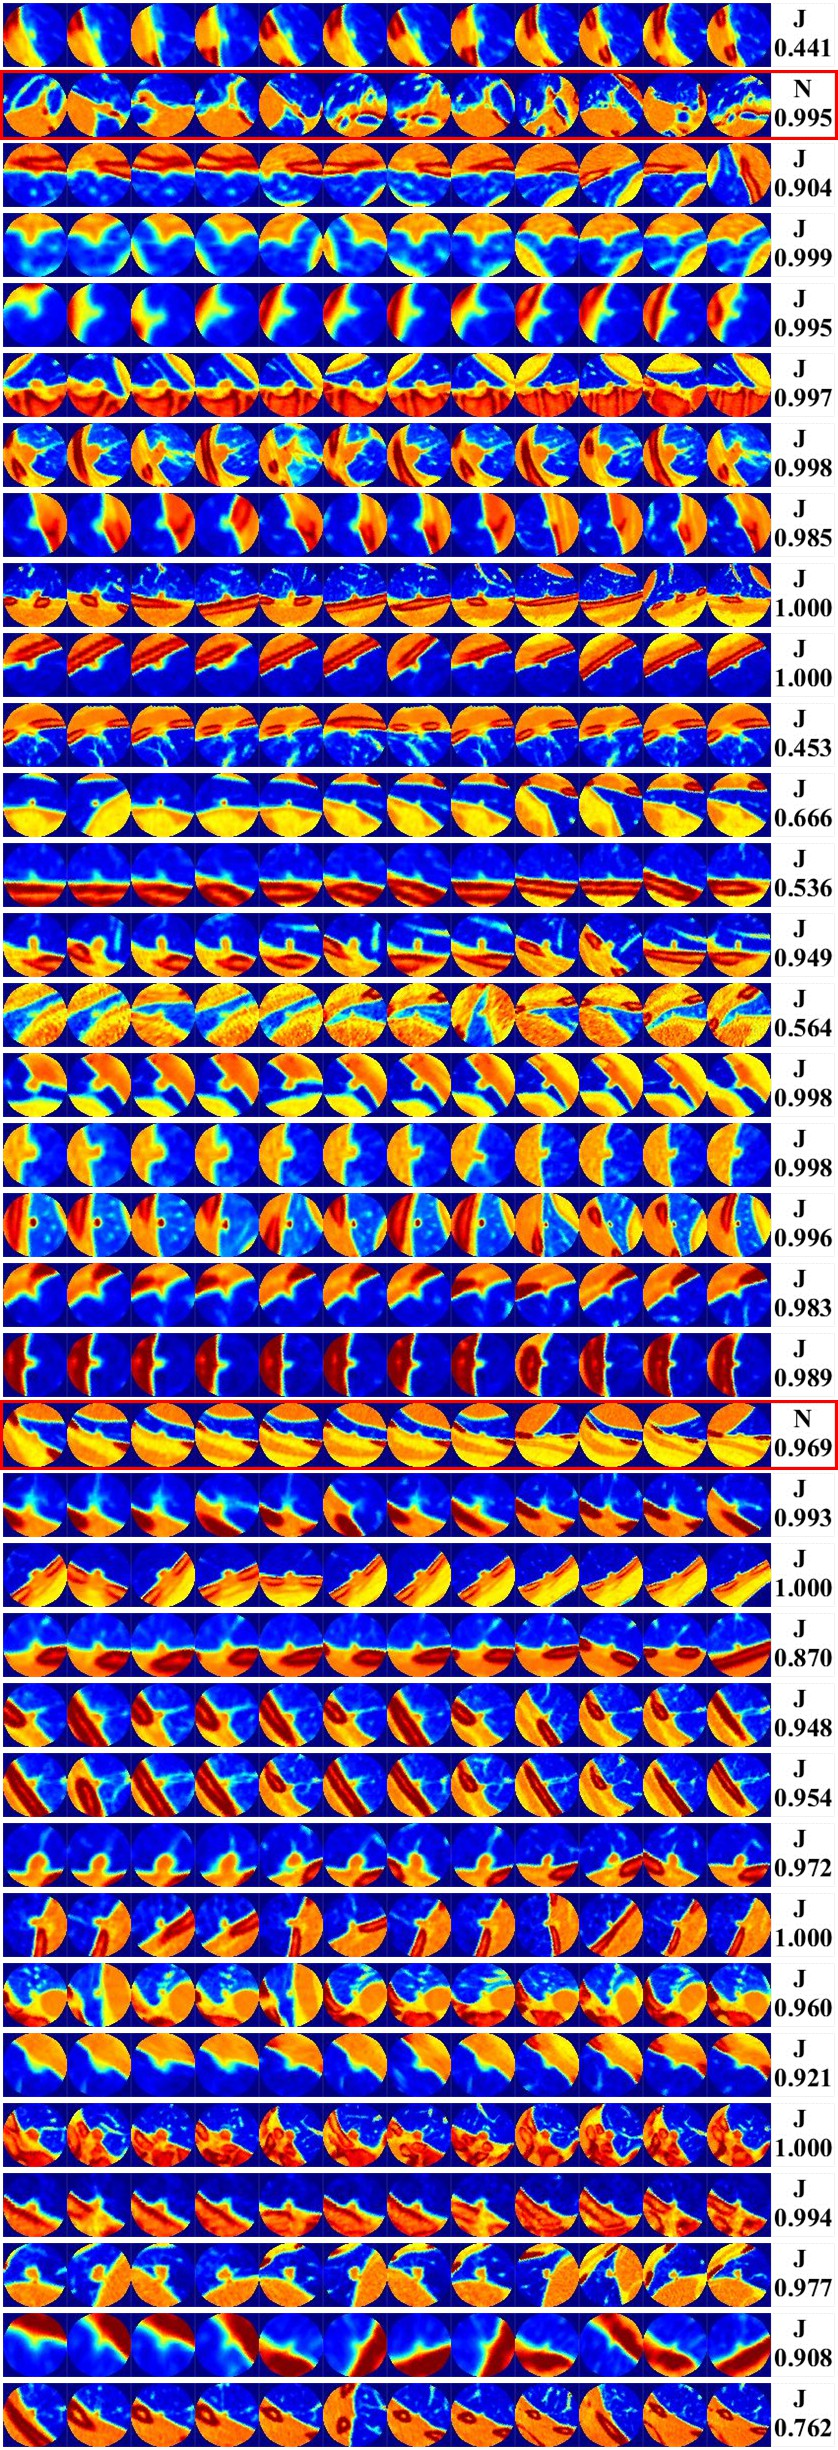
\includegraphics[width=0.45\columnwidth]{./images/lidc-msnodulecircles-wall5}
}
\end{figure}
\newpage
\begin{figure}[H]
\centering
\subfigure{
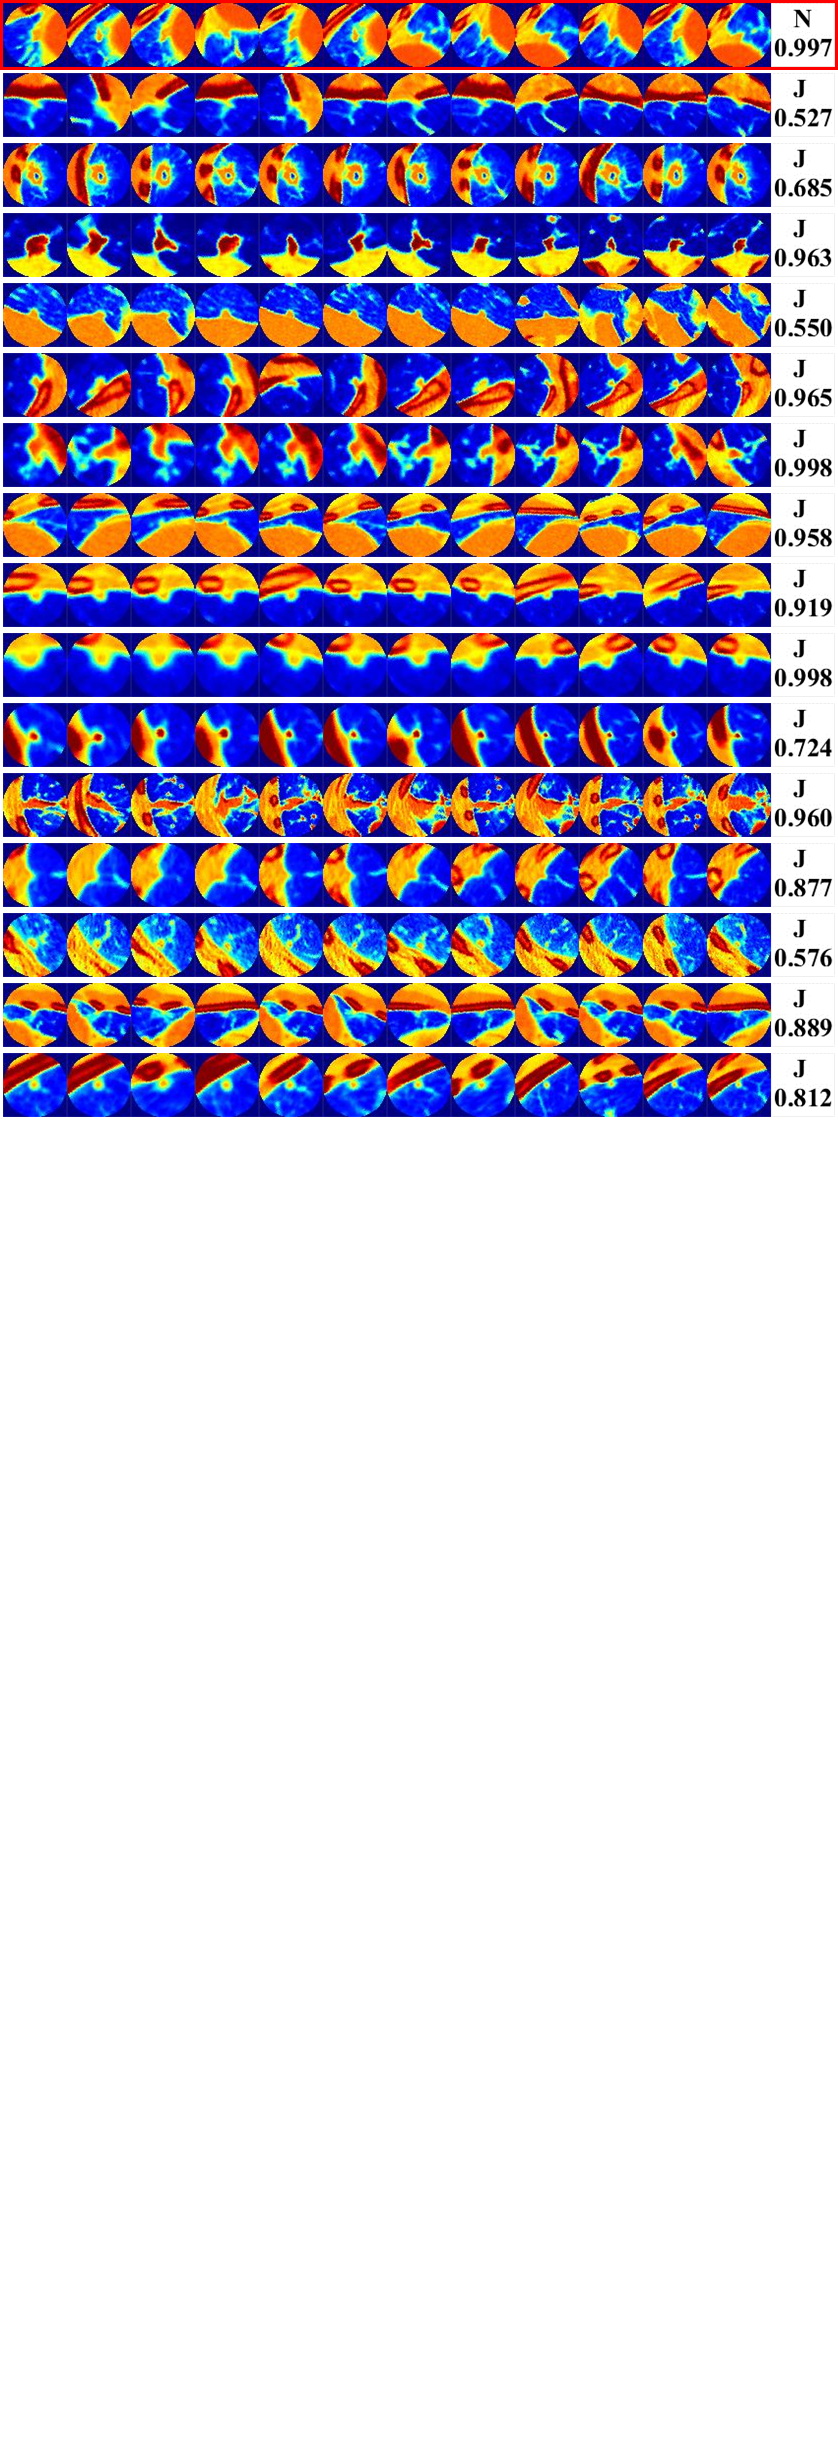
\includegraphics[width=0.45\columnwidth]{./images/lidc-msnodulecircles-wall6}
}
\end{figure}

\newpage
\subsection{Pleural-tail for \emph{ms-nodulecircles}}
\begin{figure}[H]
\centering
\subfigure{
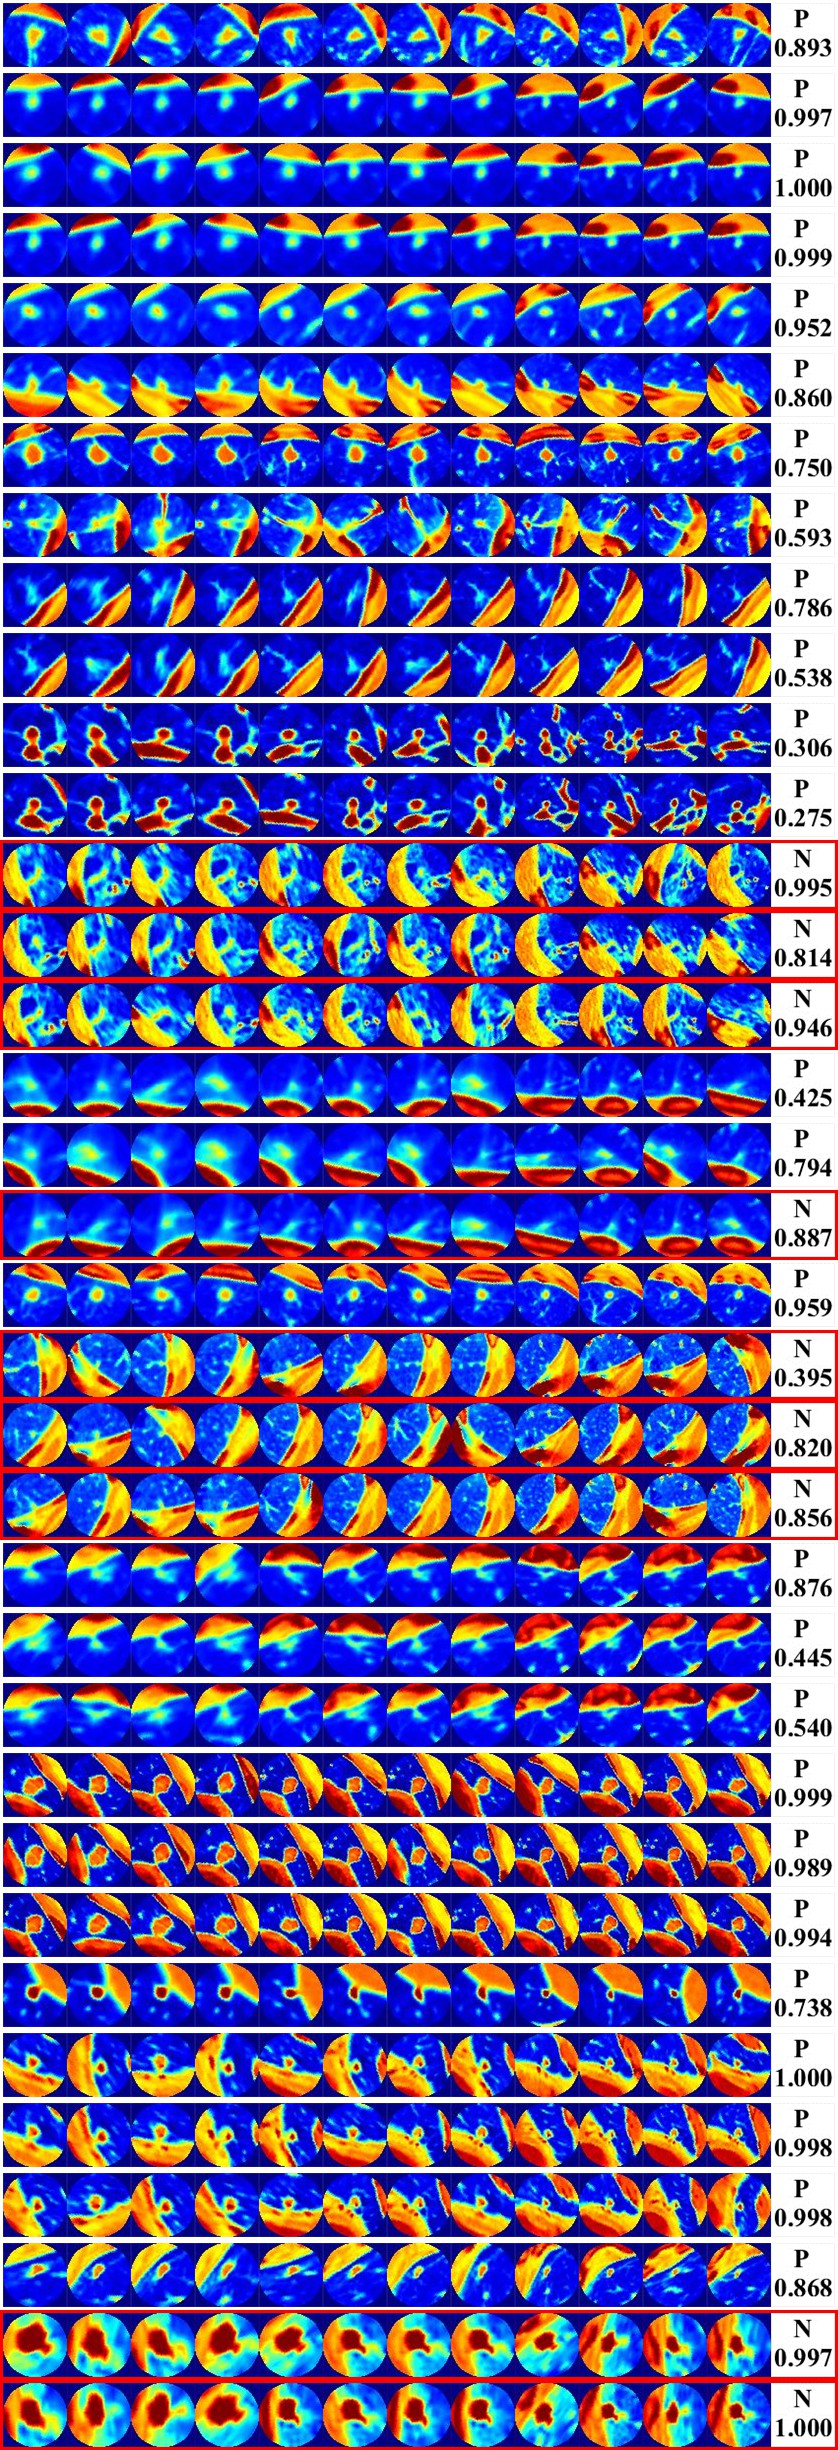
\includegraphics[width=0.45\columnwidth]{./images/lidc-msnodulecircles-tail0}
}
\hspace{.1in}
\subfigure{
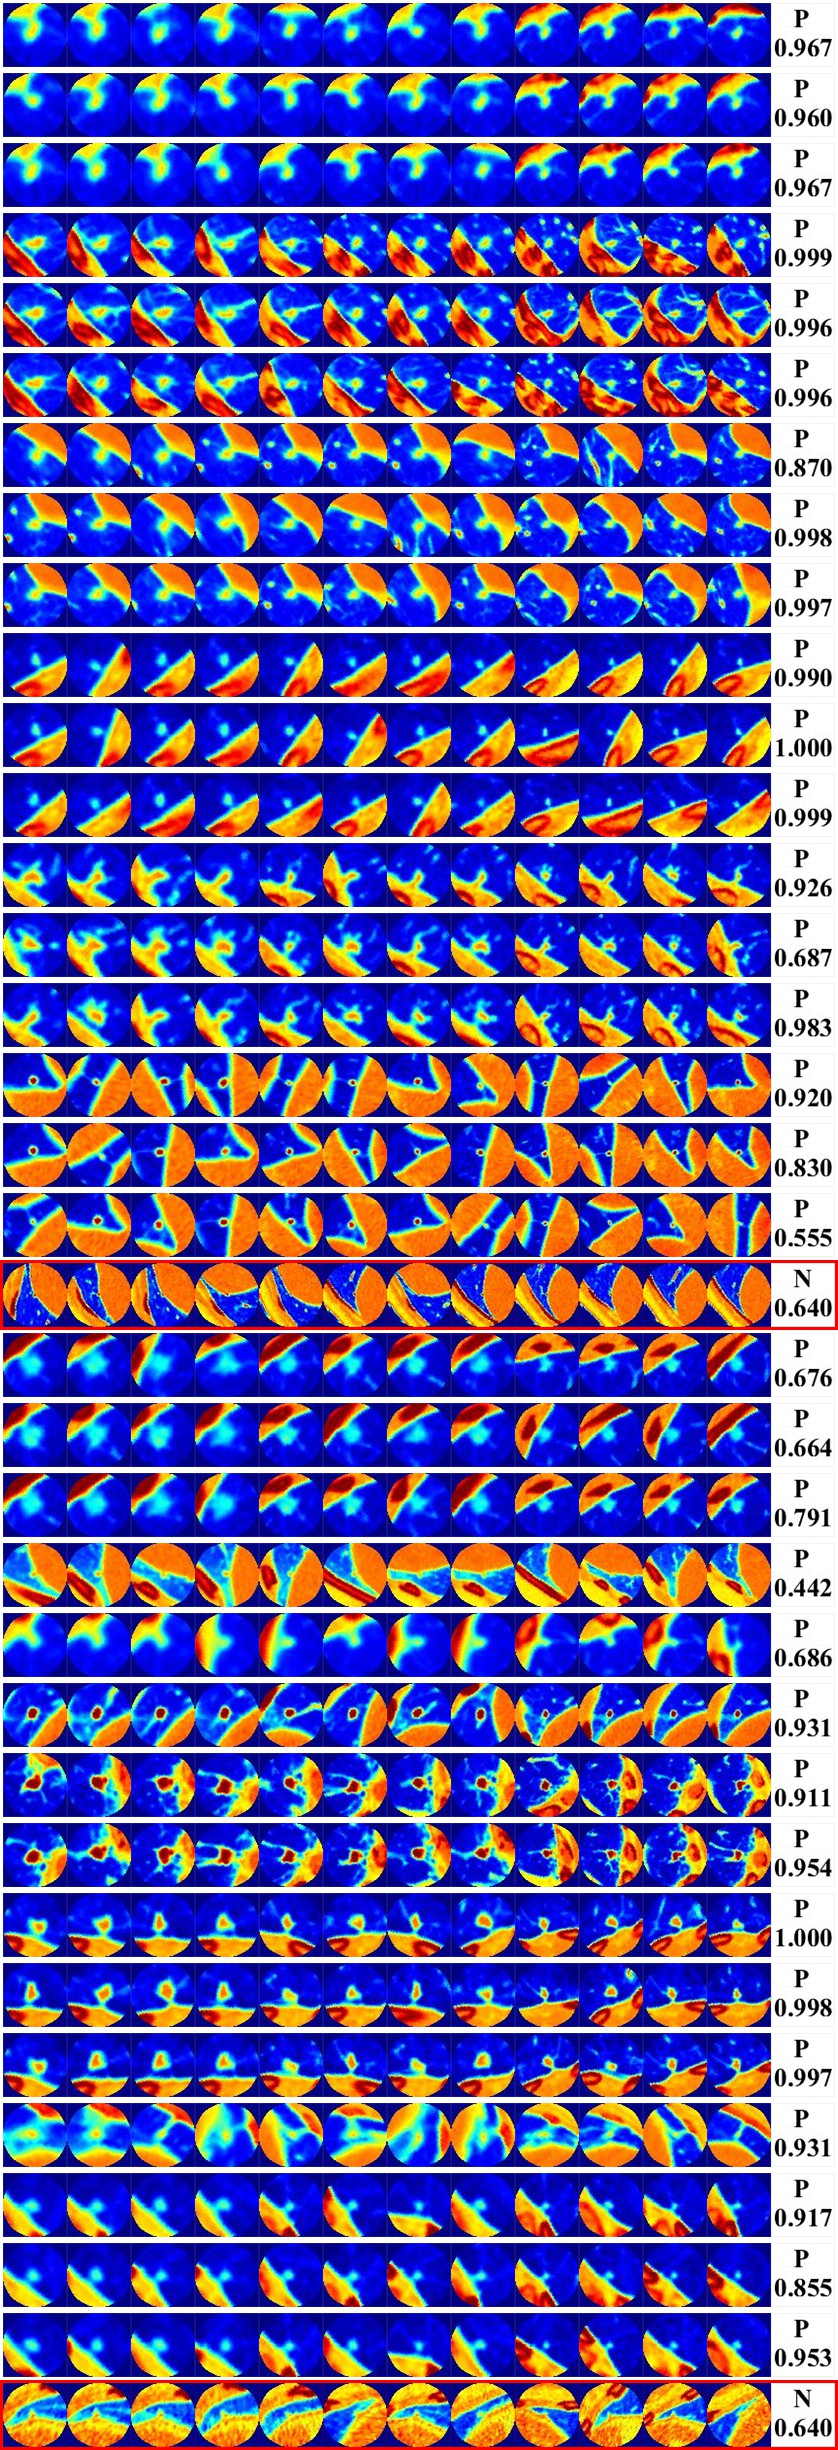
\includegraphics[width=0.45\columnwidth]{./images/lidc-msnodulecircles-tail1}
}
\end{figure}
\newpage
\begin{figure}[H]
\centering
\subfigure{
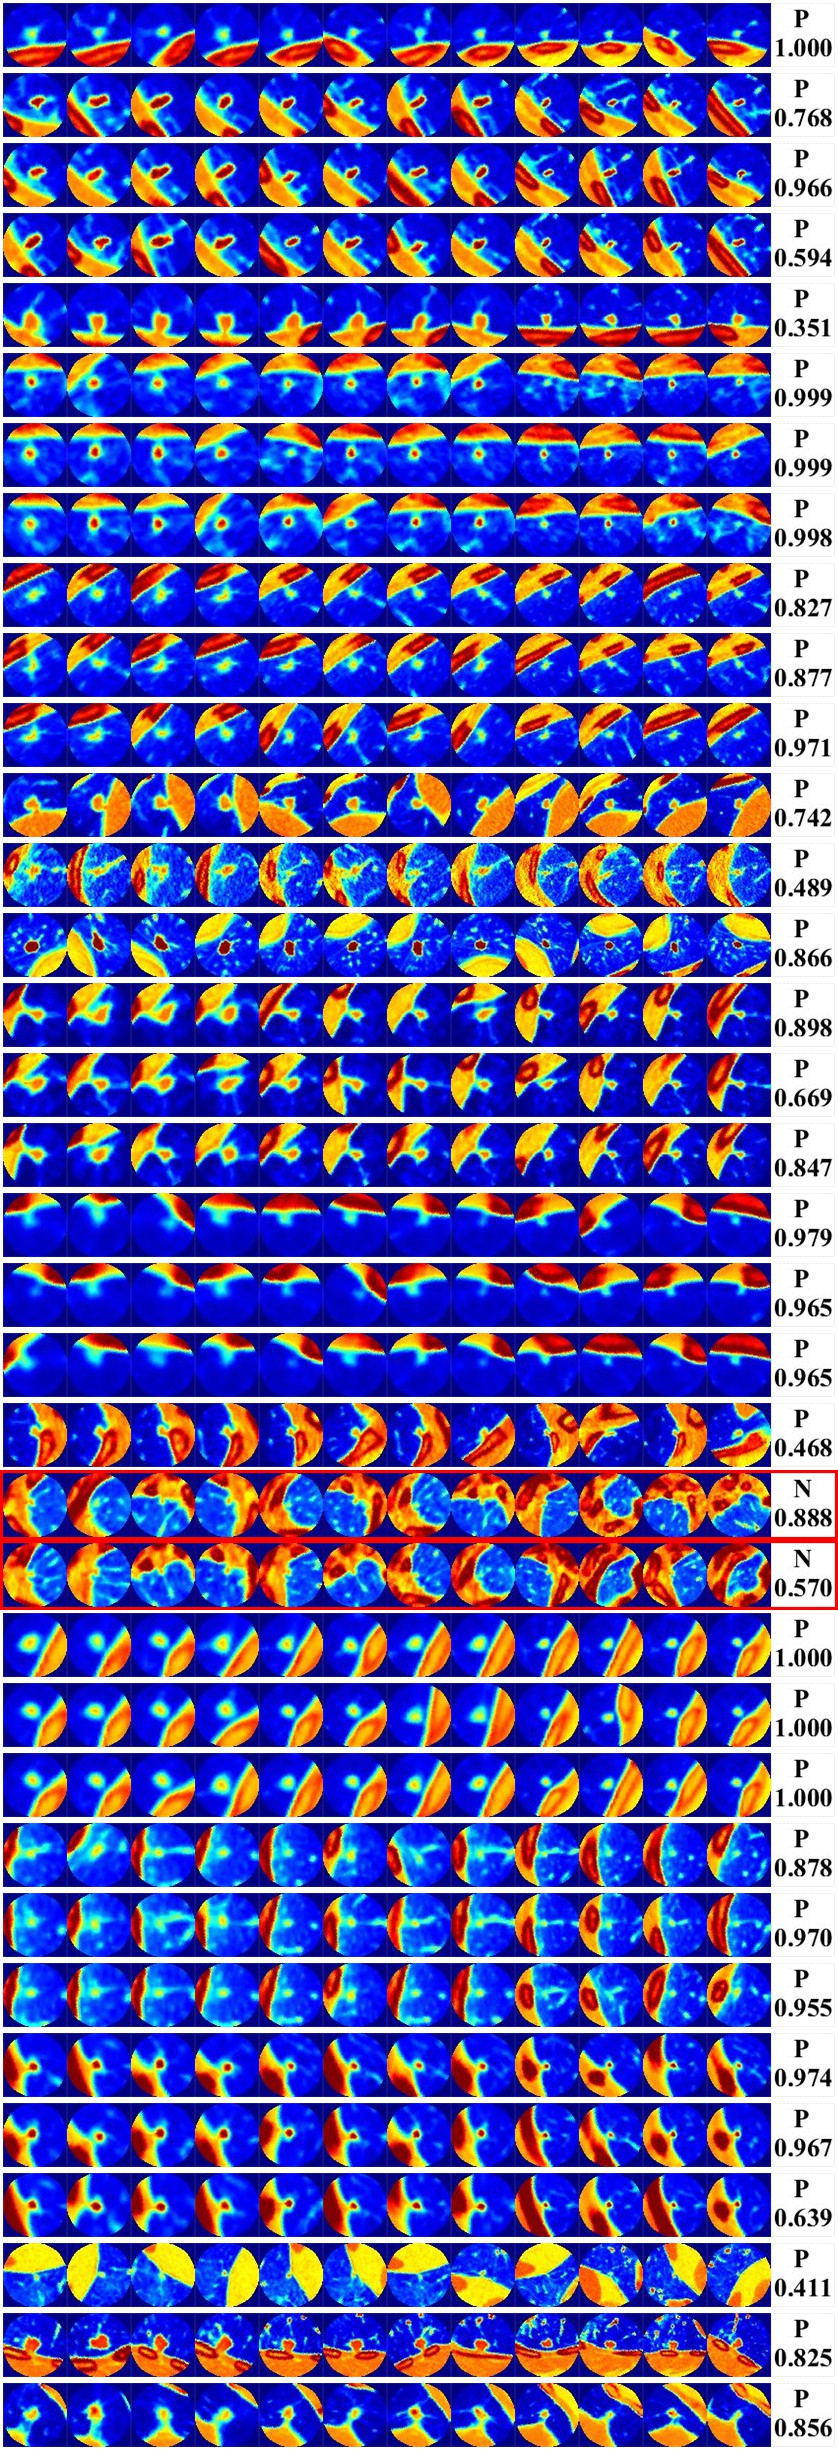
\includegraphics[width=0.45\columnwidth]{./images/lidc-msnodulecircles-tail2}
}
\hspace{.1in}
\subfigure{
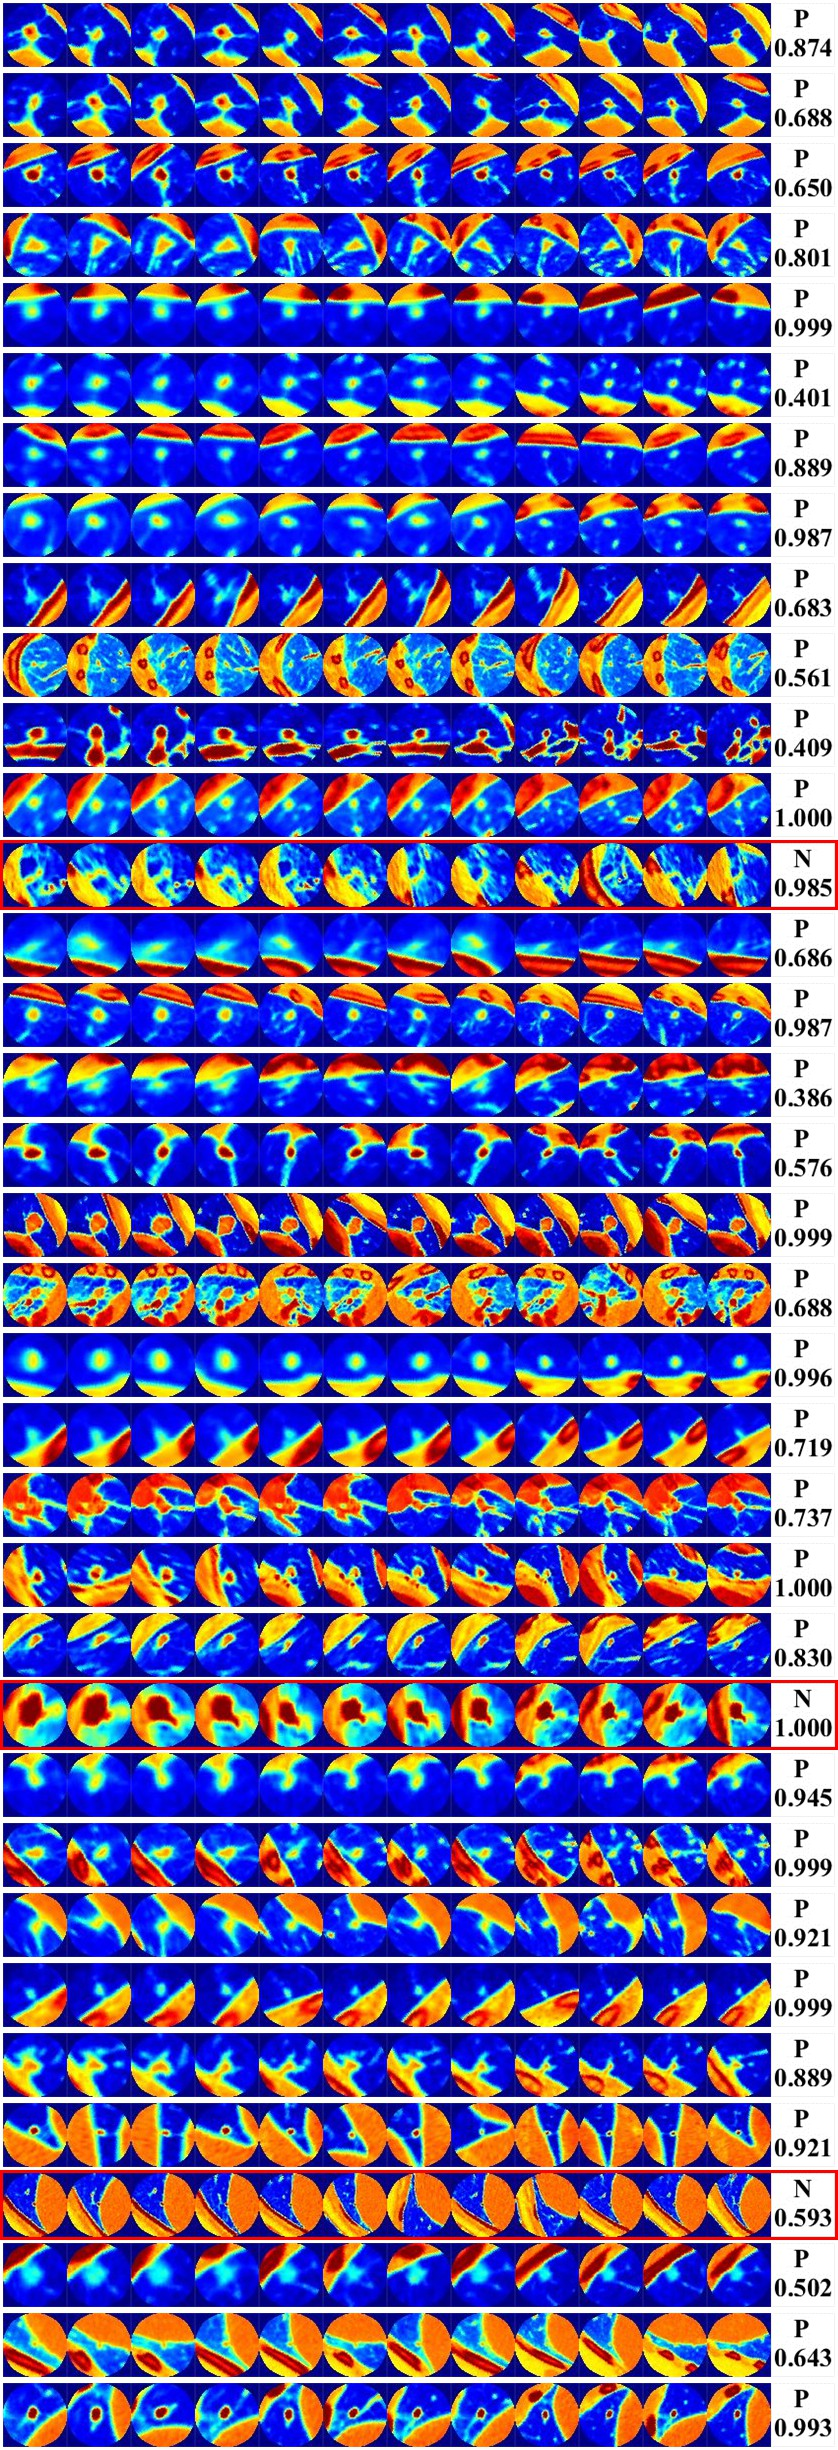
\includegraphics[width=0.45\columnwidth]{./images/lidc-msnodulecircles-tail3}
}
\end{figure}
\newpage
\begin{figure}[H]
\centering
\subfigure{
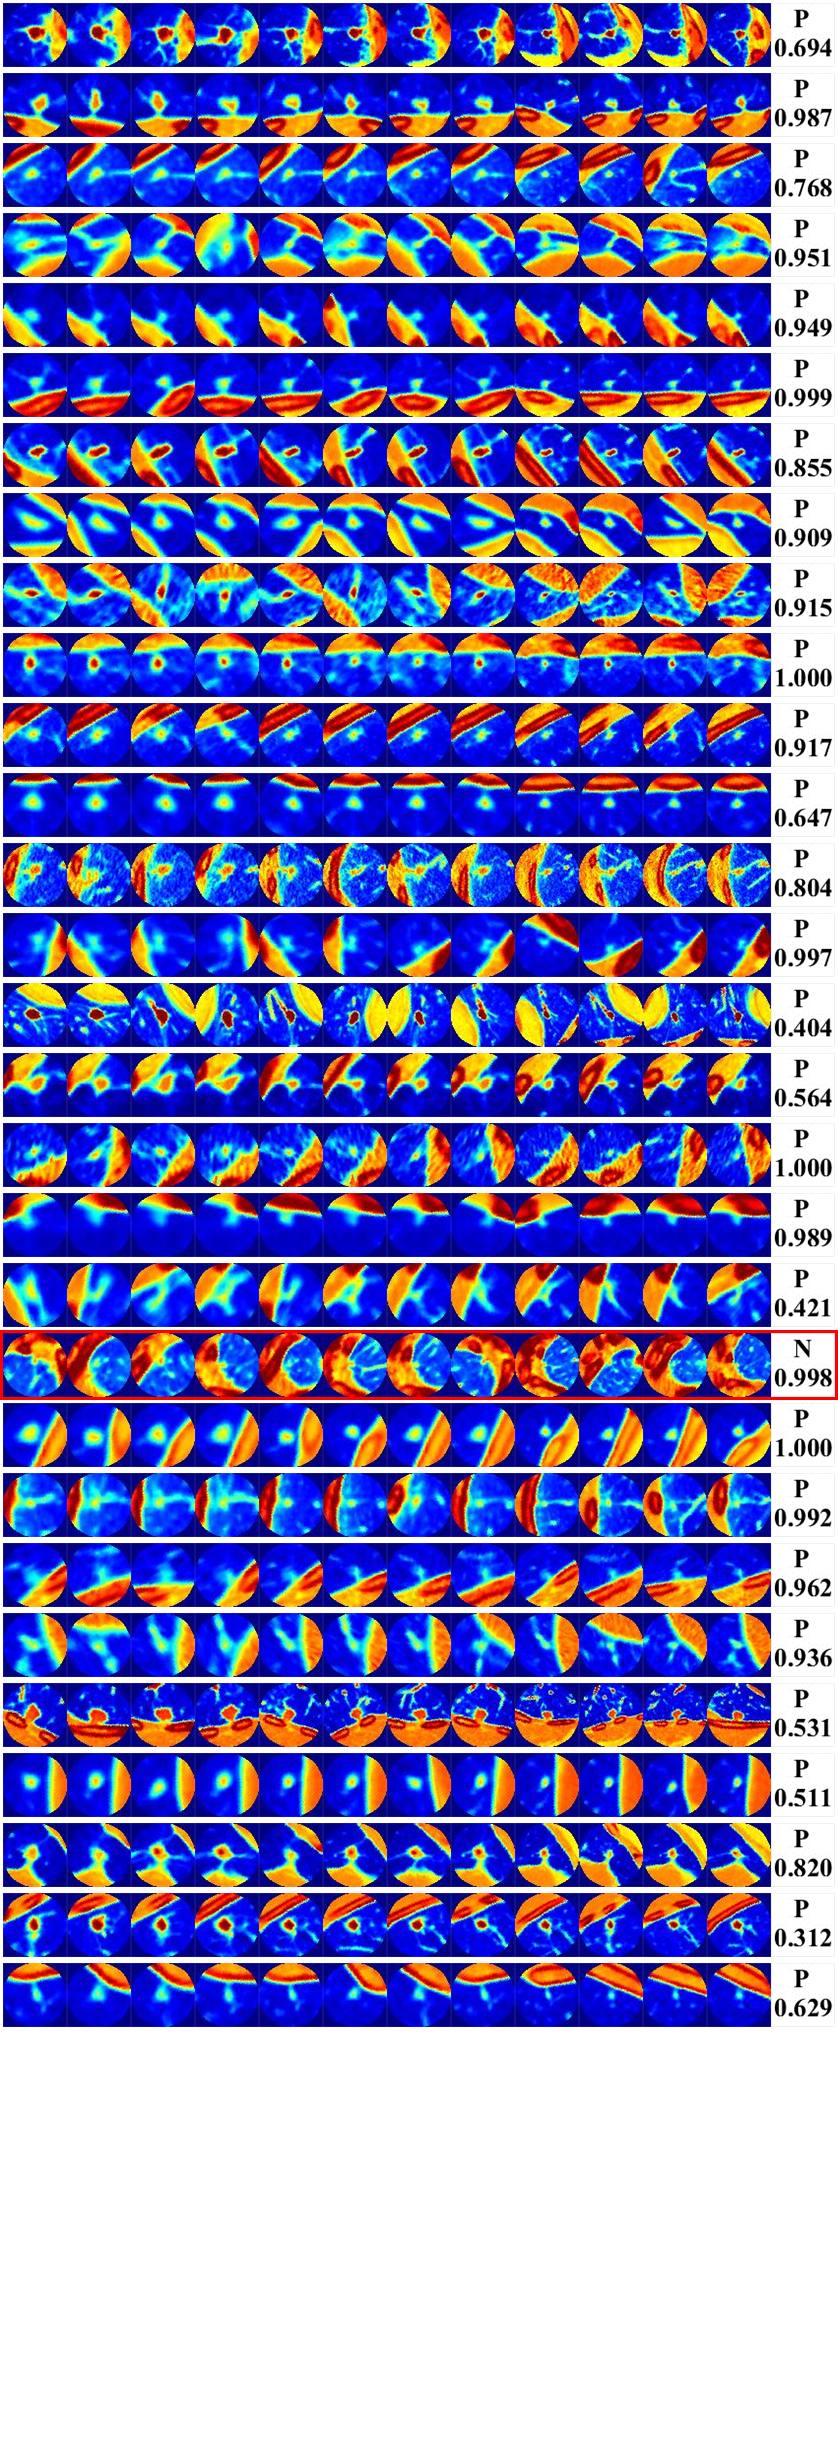
\includegraphics[width=0.45\columnwidth]{./images/lidc-msnodulecircles-tail4}
}
\end{figure}

\newpage
\subsection{Vascularized for \emph{ms-nodulecircles}}
\begin{figure}[H]
\centering
\subfigure{
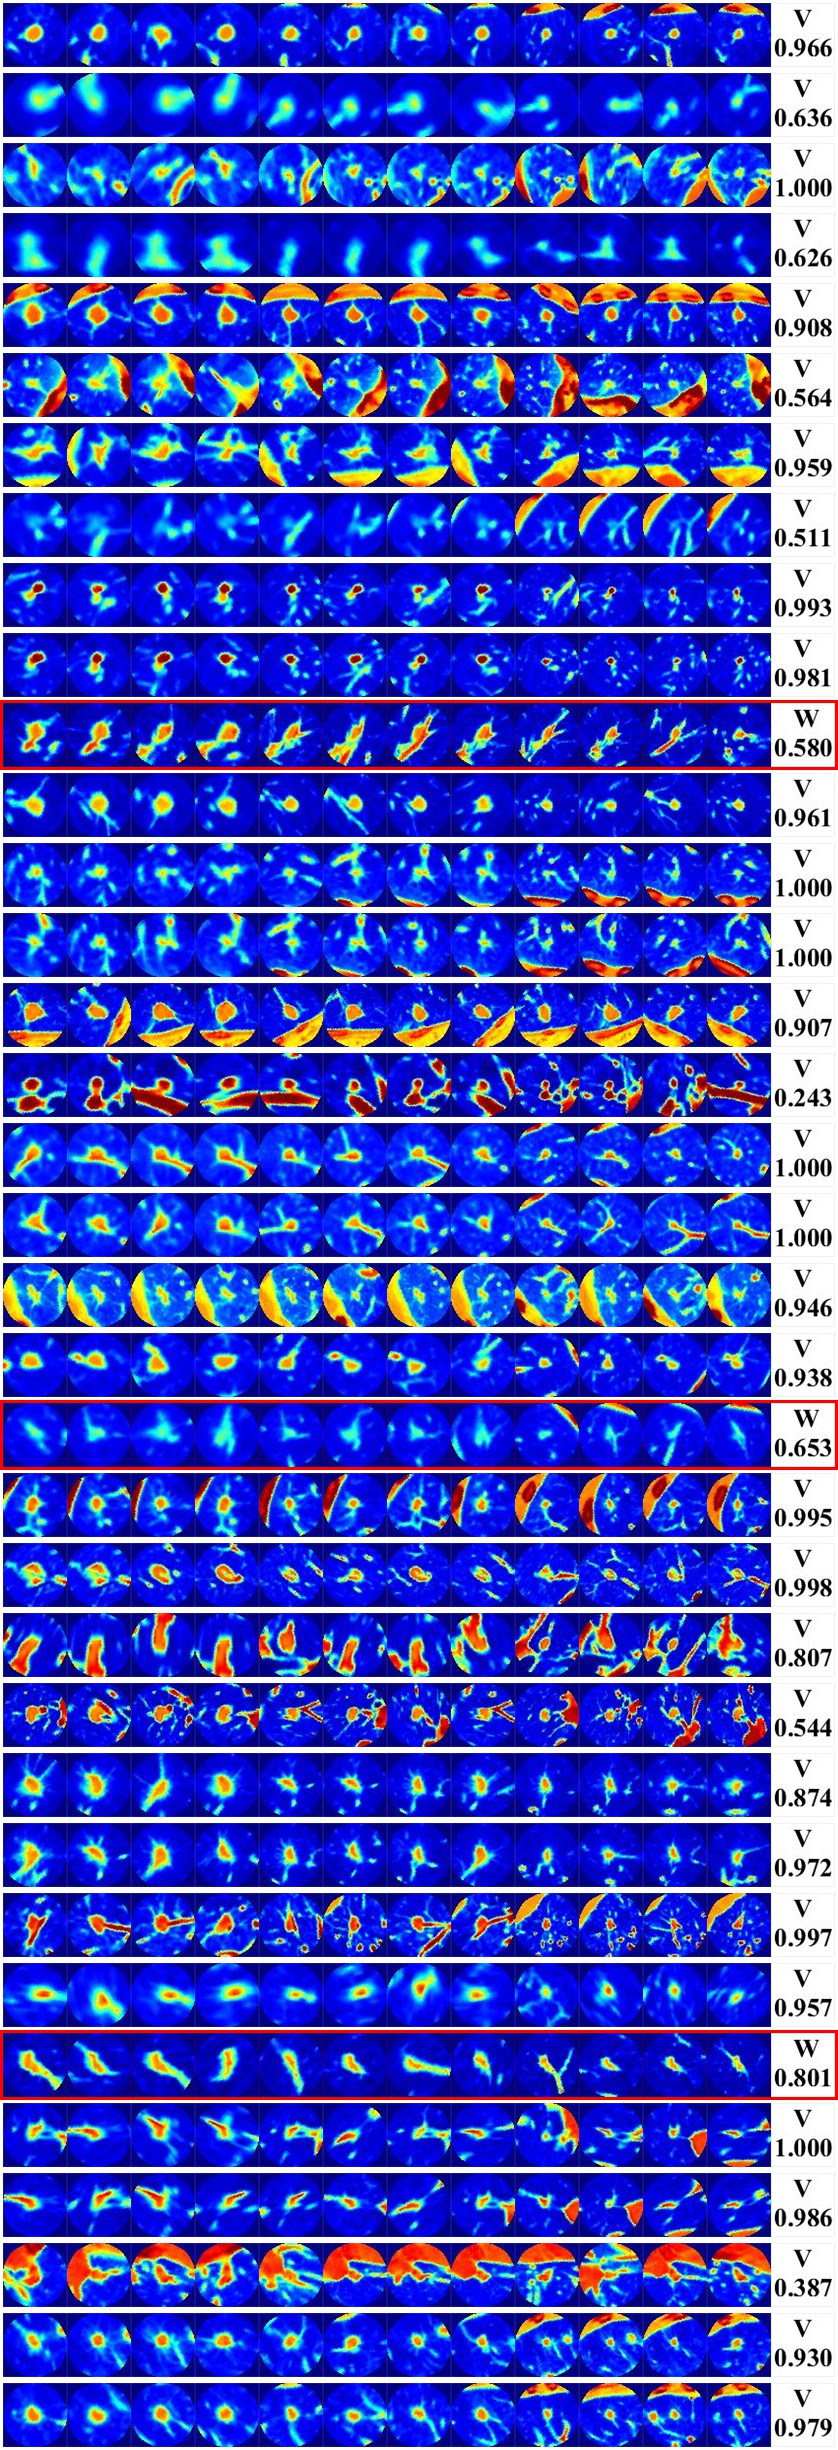
\includegraphics[width=0.45\columnwidth]{./images/lidc-msnodulecircles-vessel0}
}
\hspace{.1in}
\subfigure{
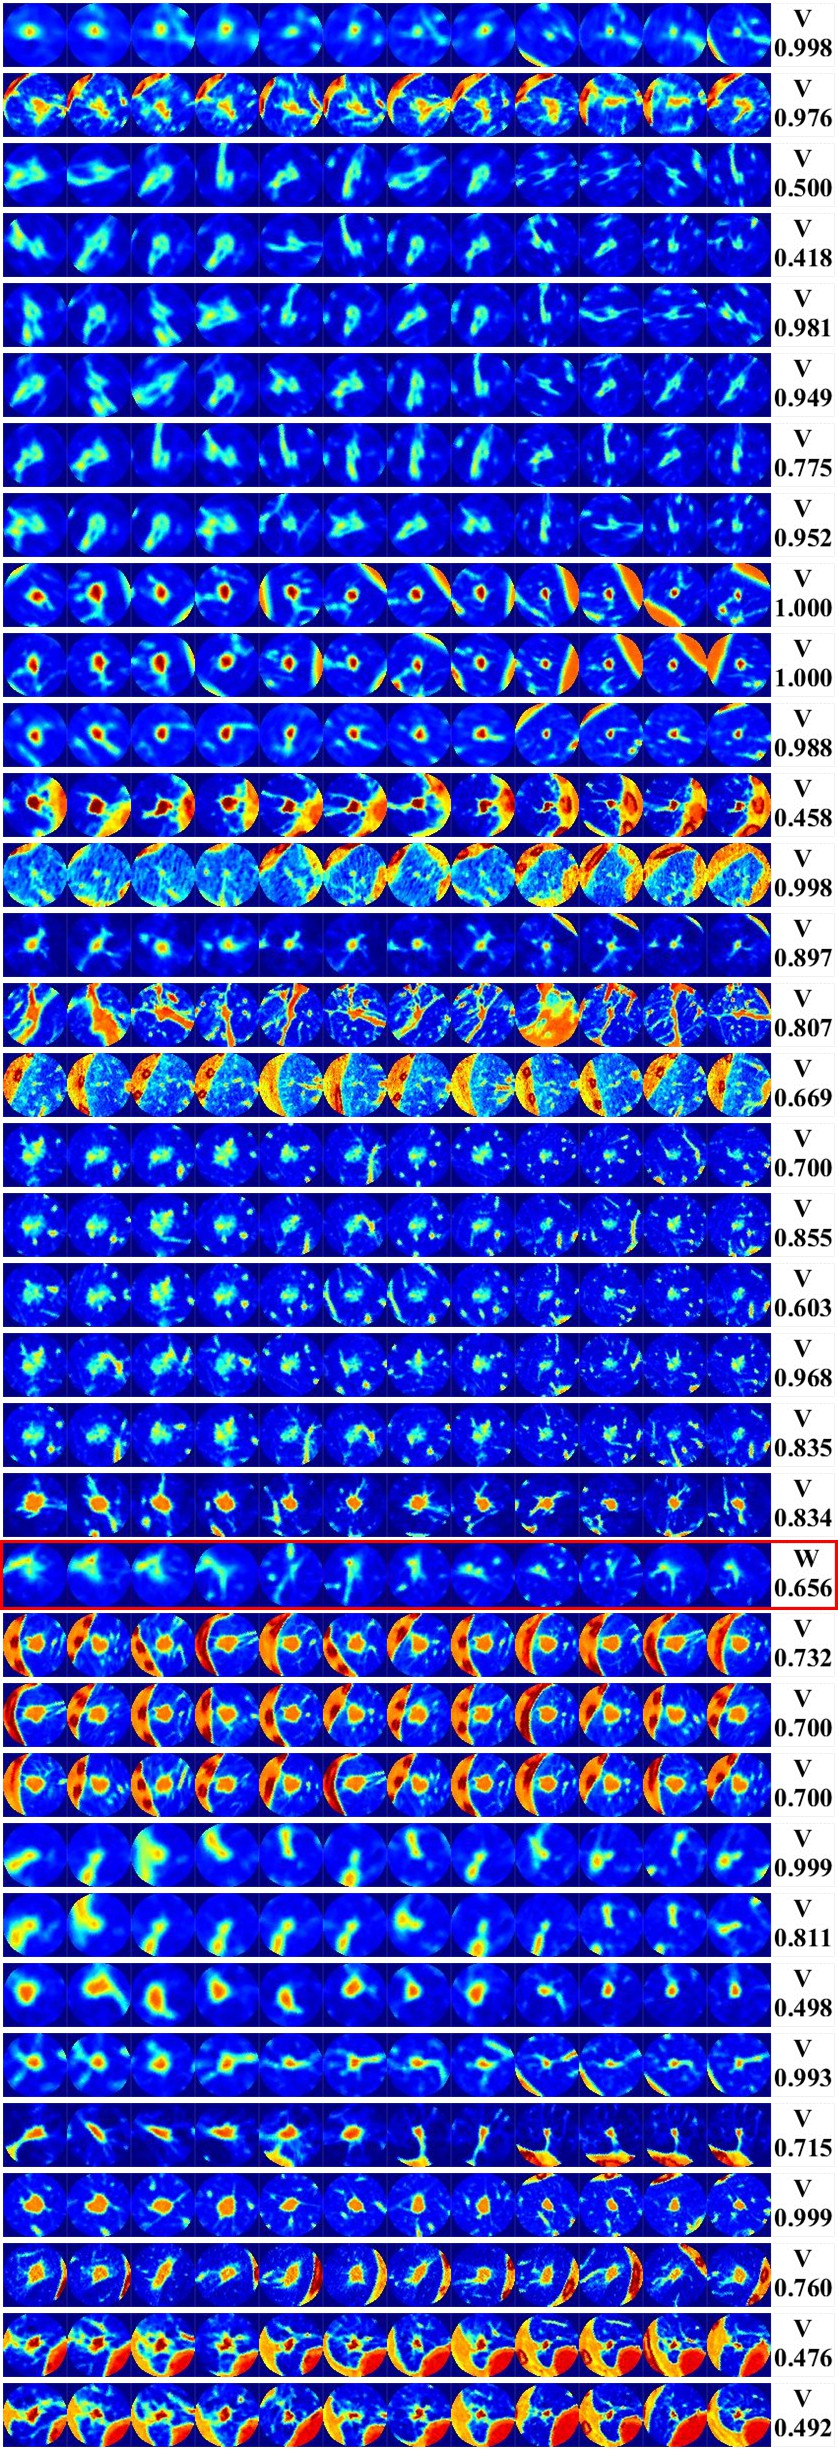
\includegraphics[width=0.45\columnwidth]{./images/lidc-msnodulecircles-vessel1}
}
\end{figure}
\newpage
\begin{figure}[H]
\centering
\subfigure{
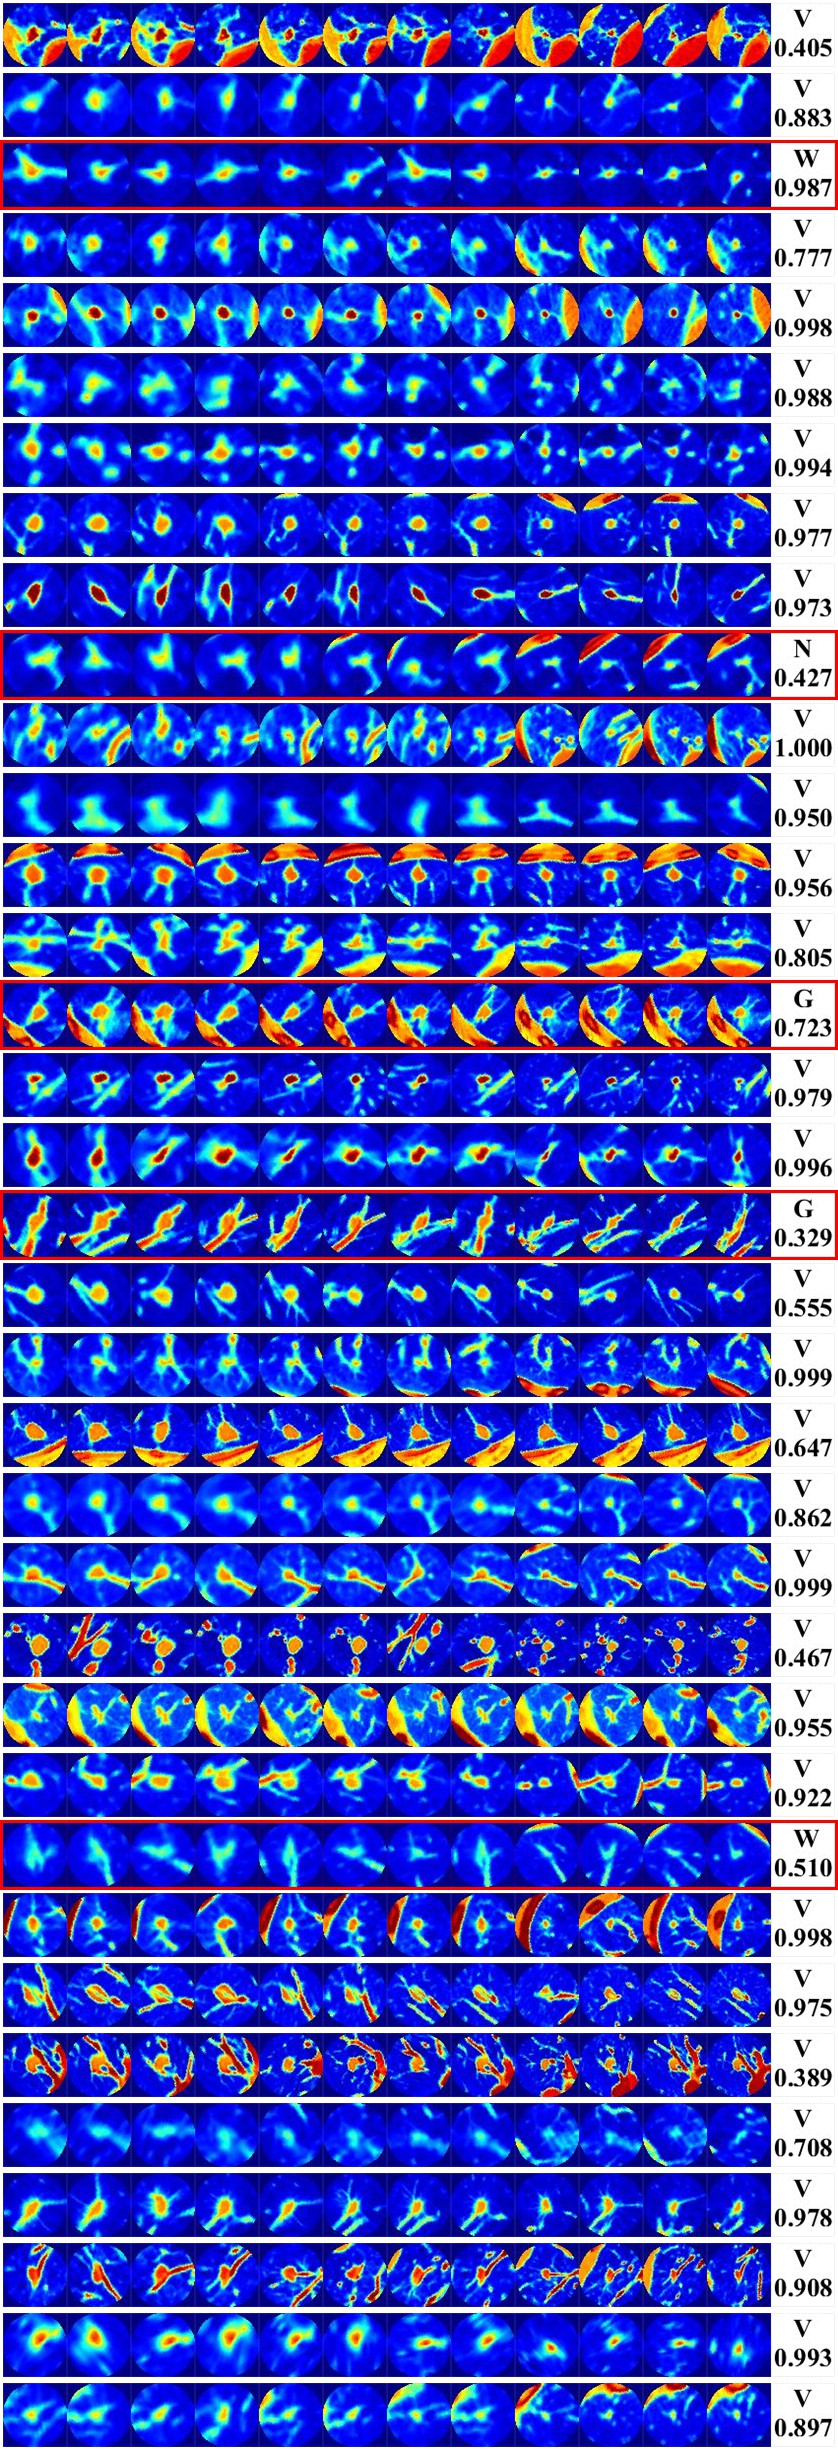
\includegraphics[width=0.45\columnwidth]{./images/lidc-msnodulecircles-vessel2}
}
\hspace{.1in}
\subfigure{
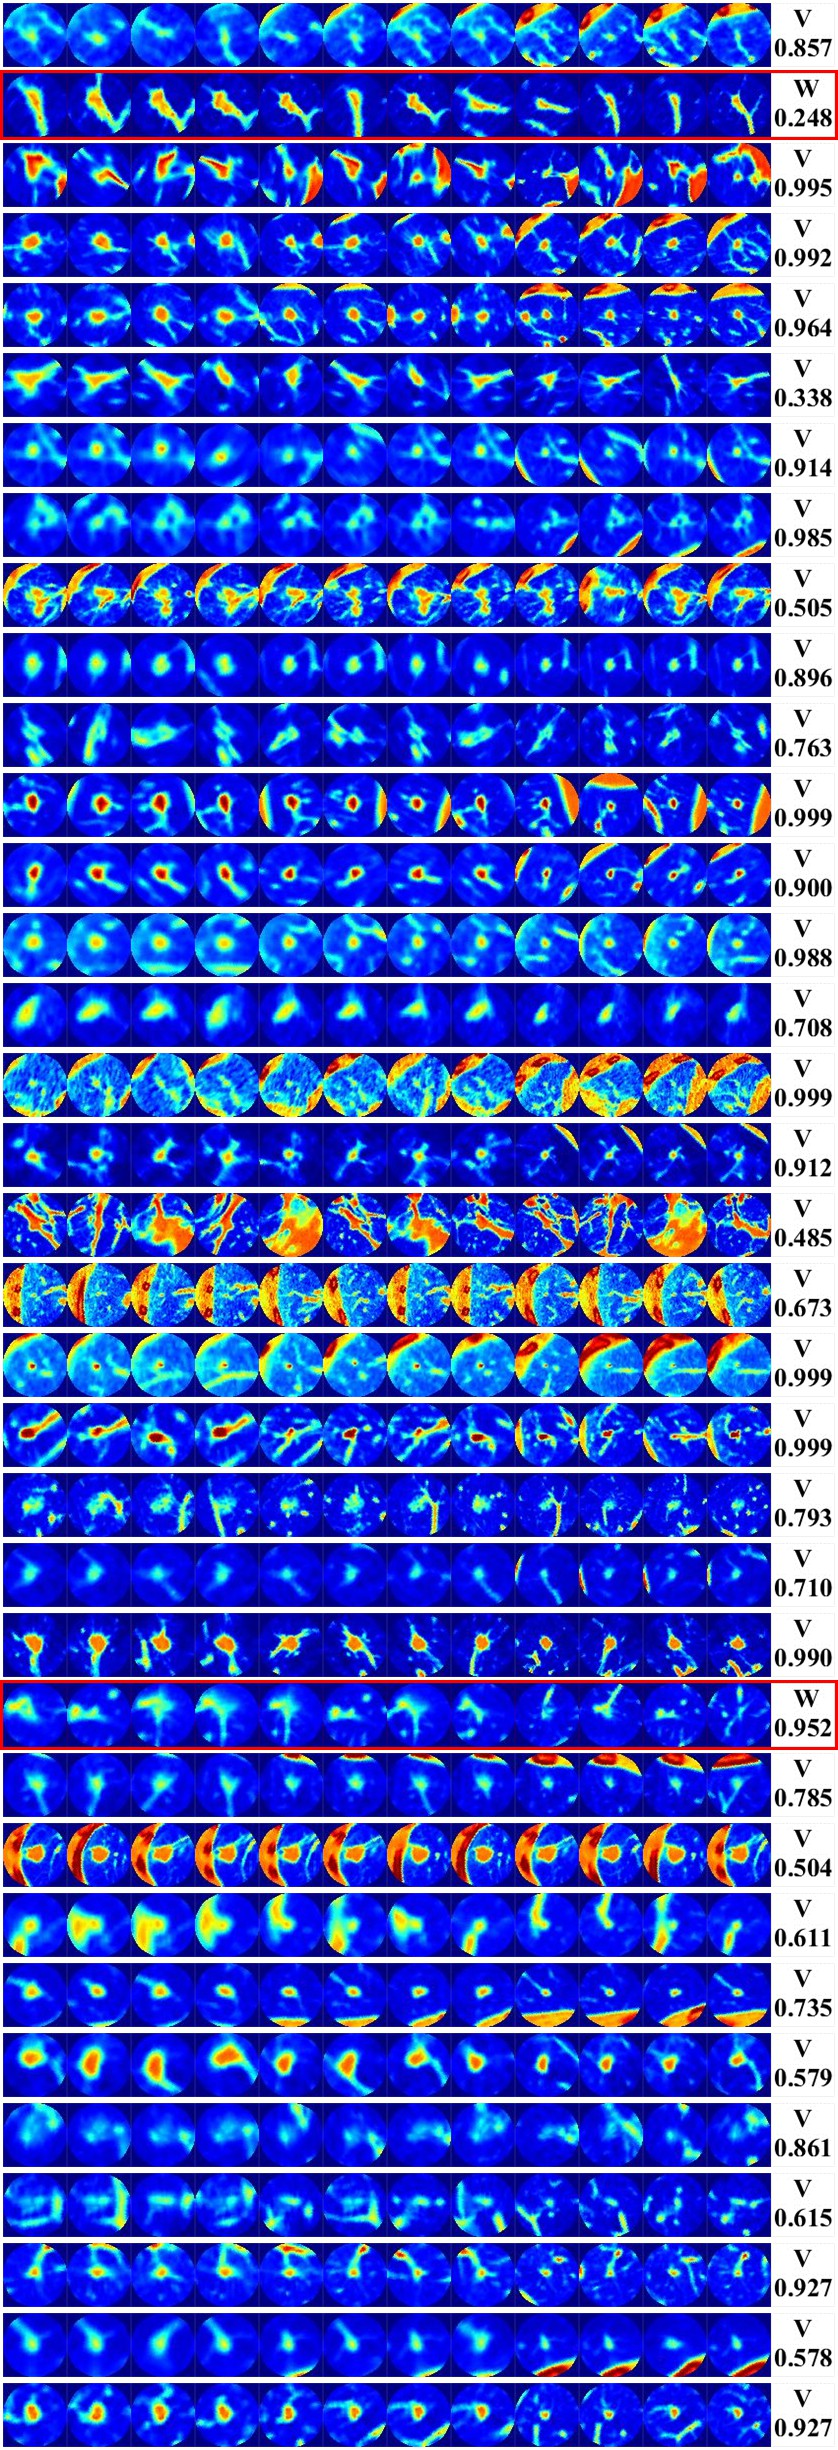
\includegraphics[width=0.45\columnwidth]{./images/lidc-msnodulecircles-vessel3}
}
\end{figure}
\newpage
\begin{figure}[H]
\centering
\subfigure{
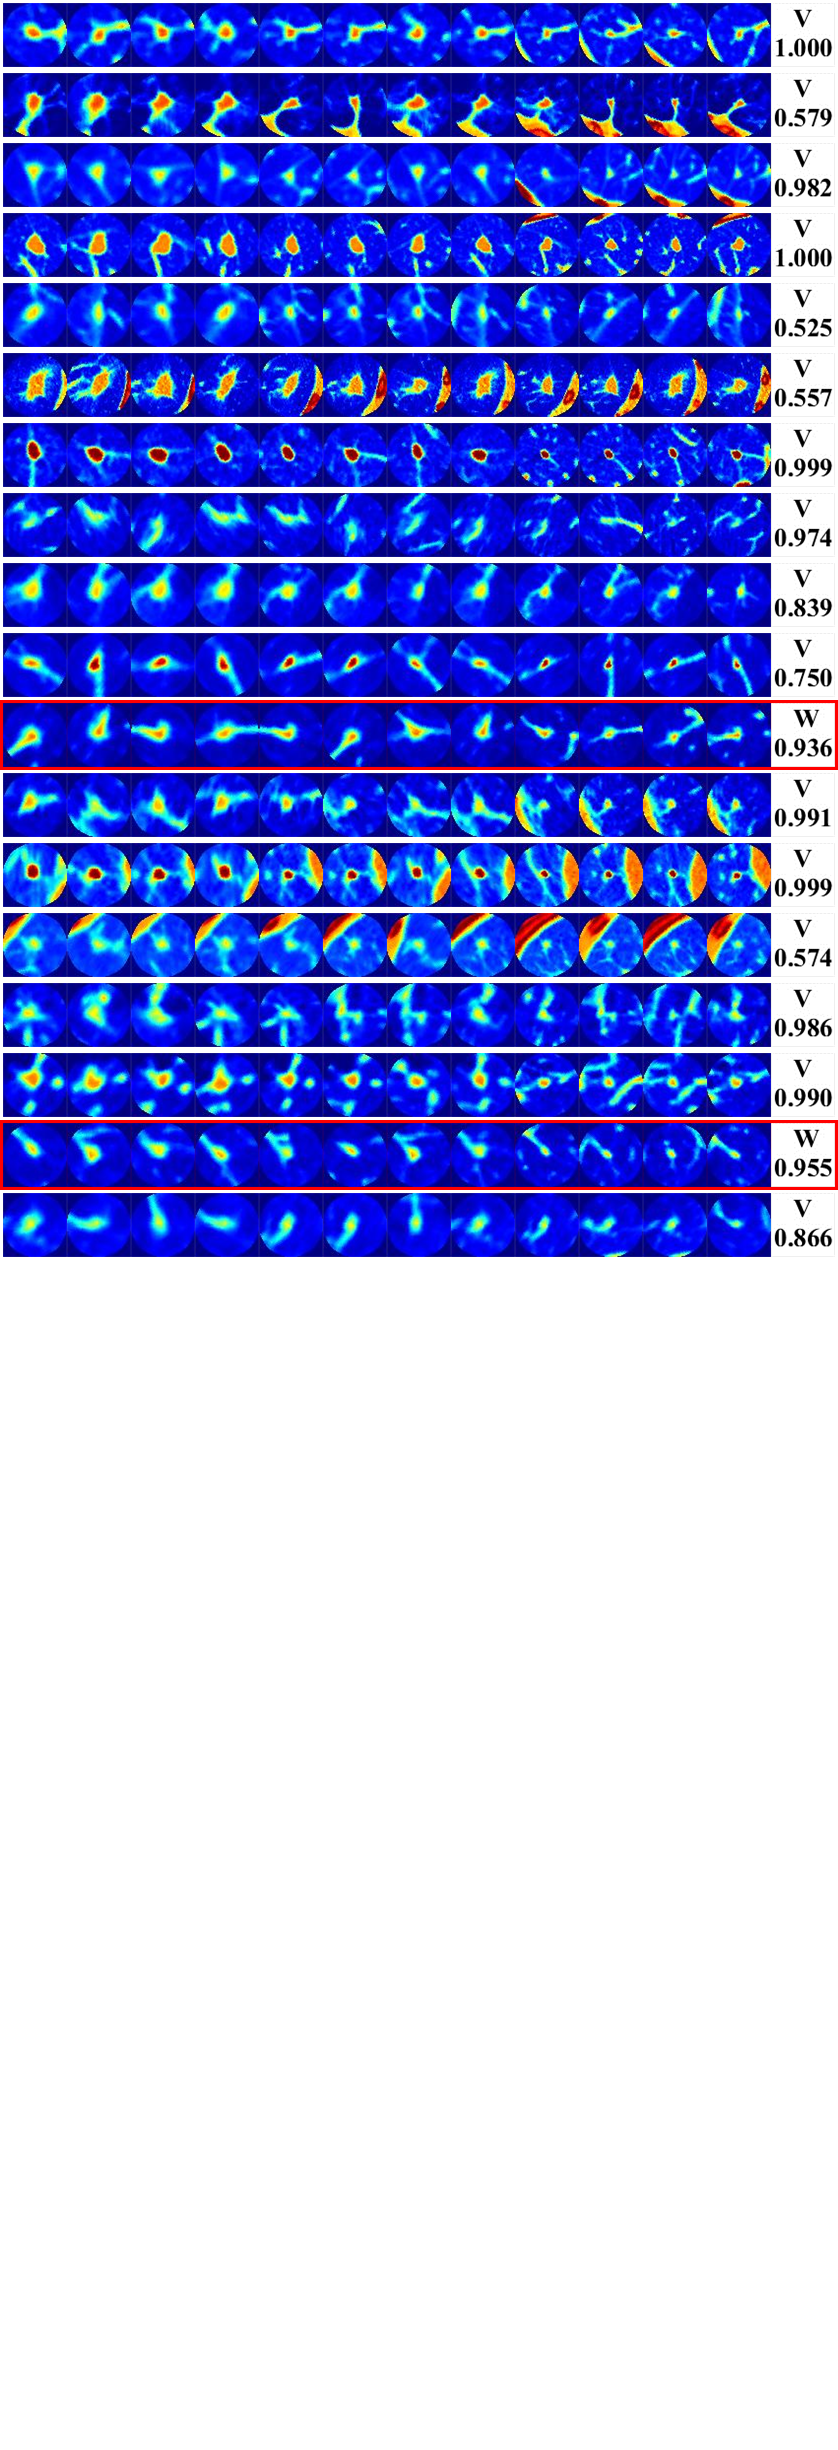
\includegraphics[width=0.45\columnwidth]{./images/lidc-msnodulecircles-vessel4}
}
\end{figure}


\newpage
\subsection{NON-NODULE for \emph{ms-nodulecircles}}
\begin{figure}[H]
\centering
\subfigure{
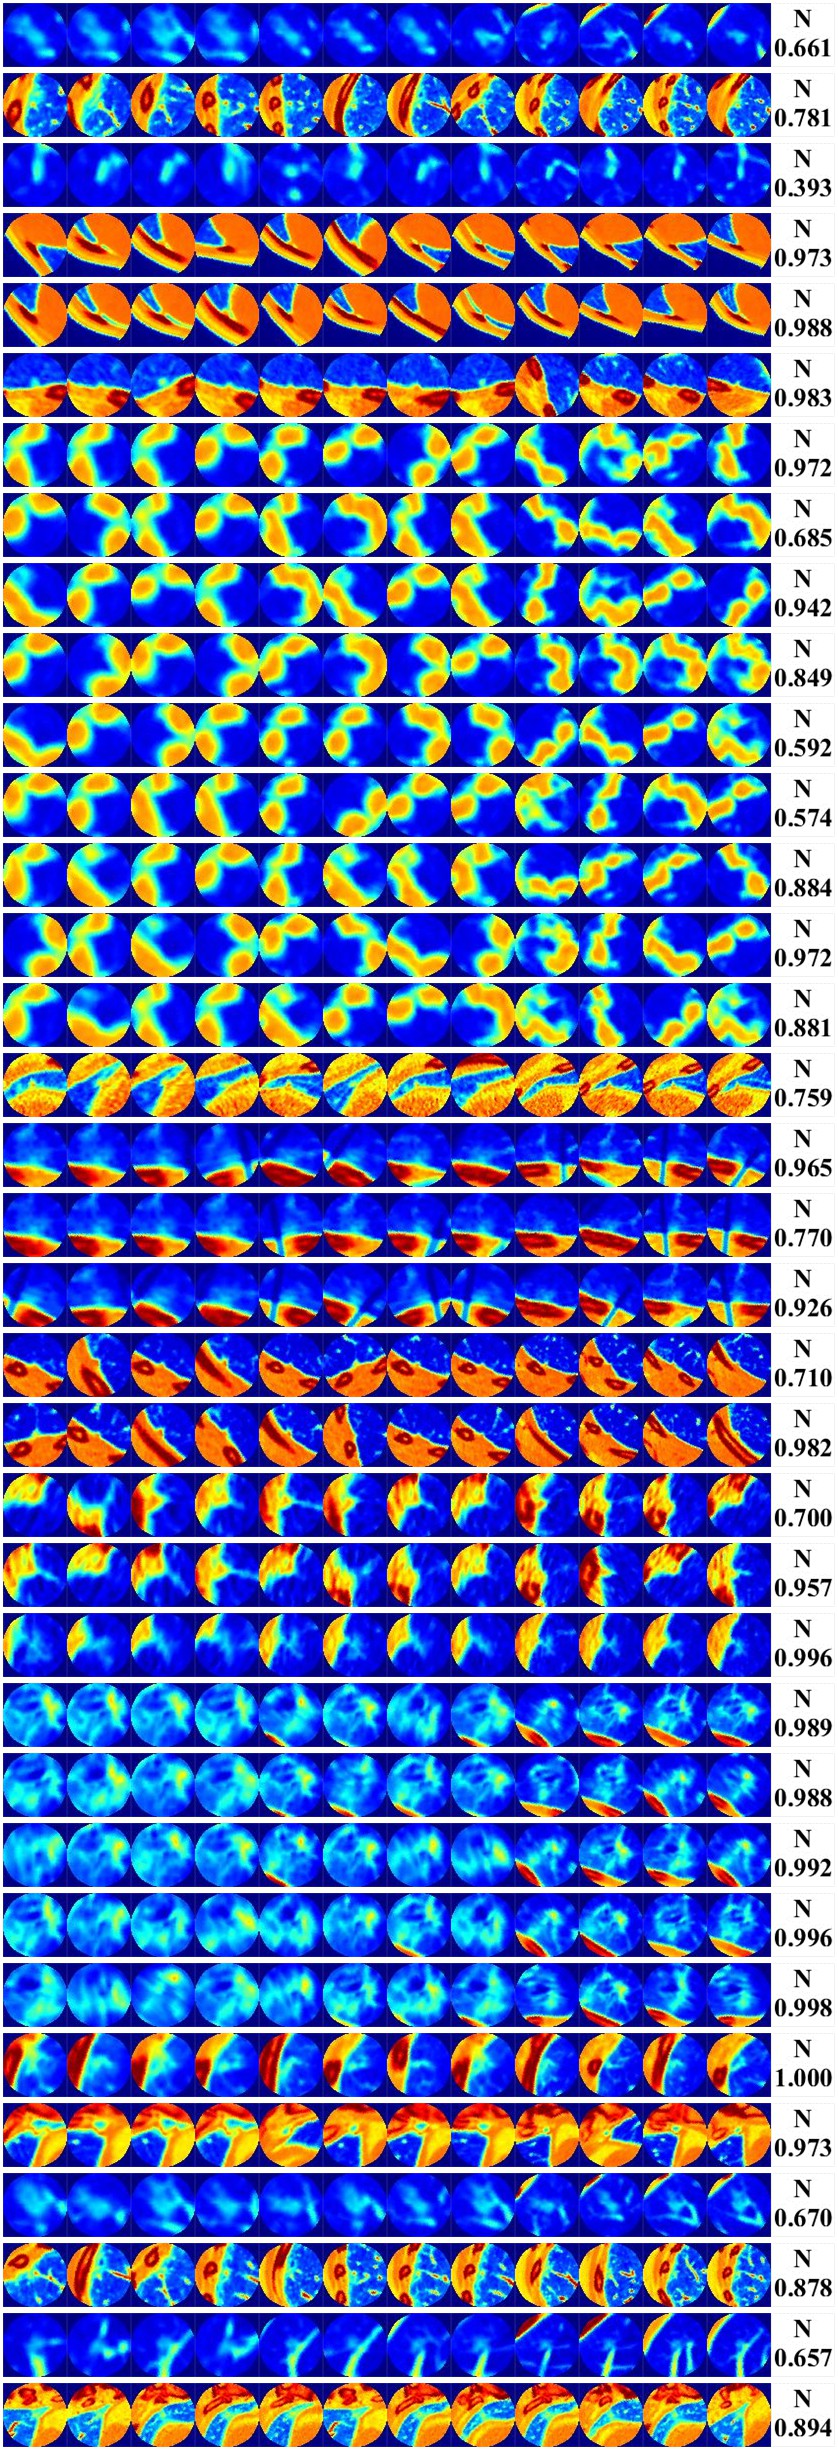
\includegraphics[width=0.45\columnwidth]{./images/lidc-msnodulecircles-nonnodule0}
}
\hspace{.1in}
\subfigure{
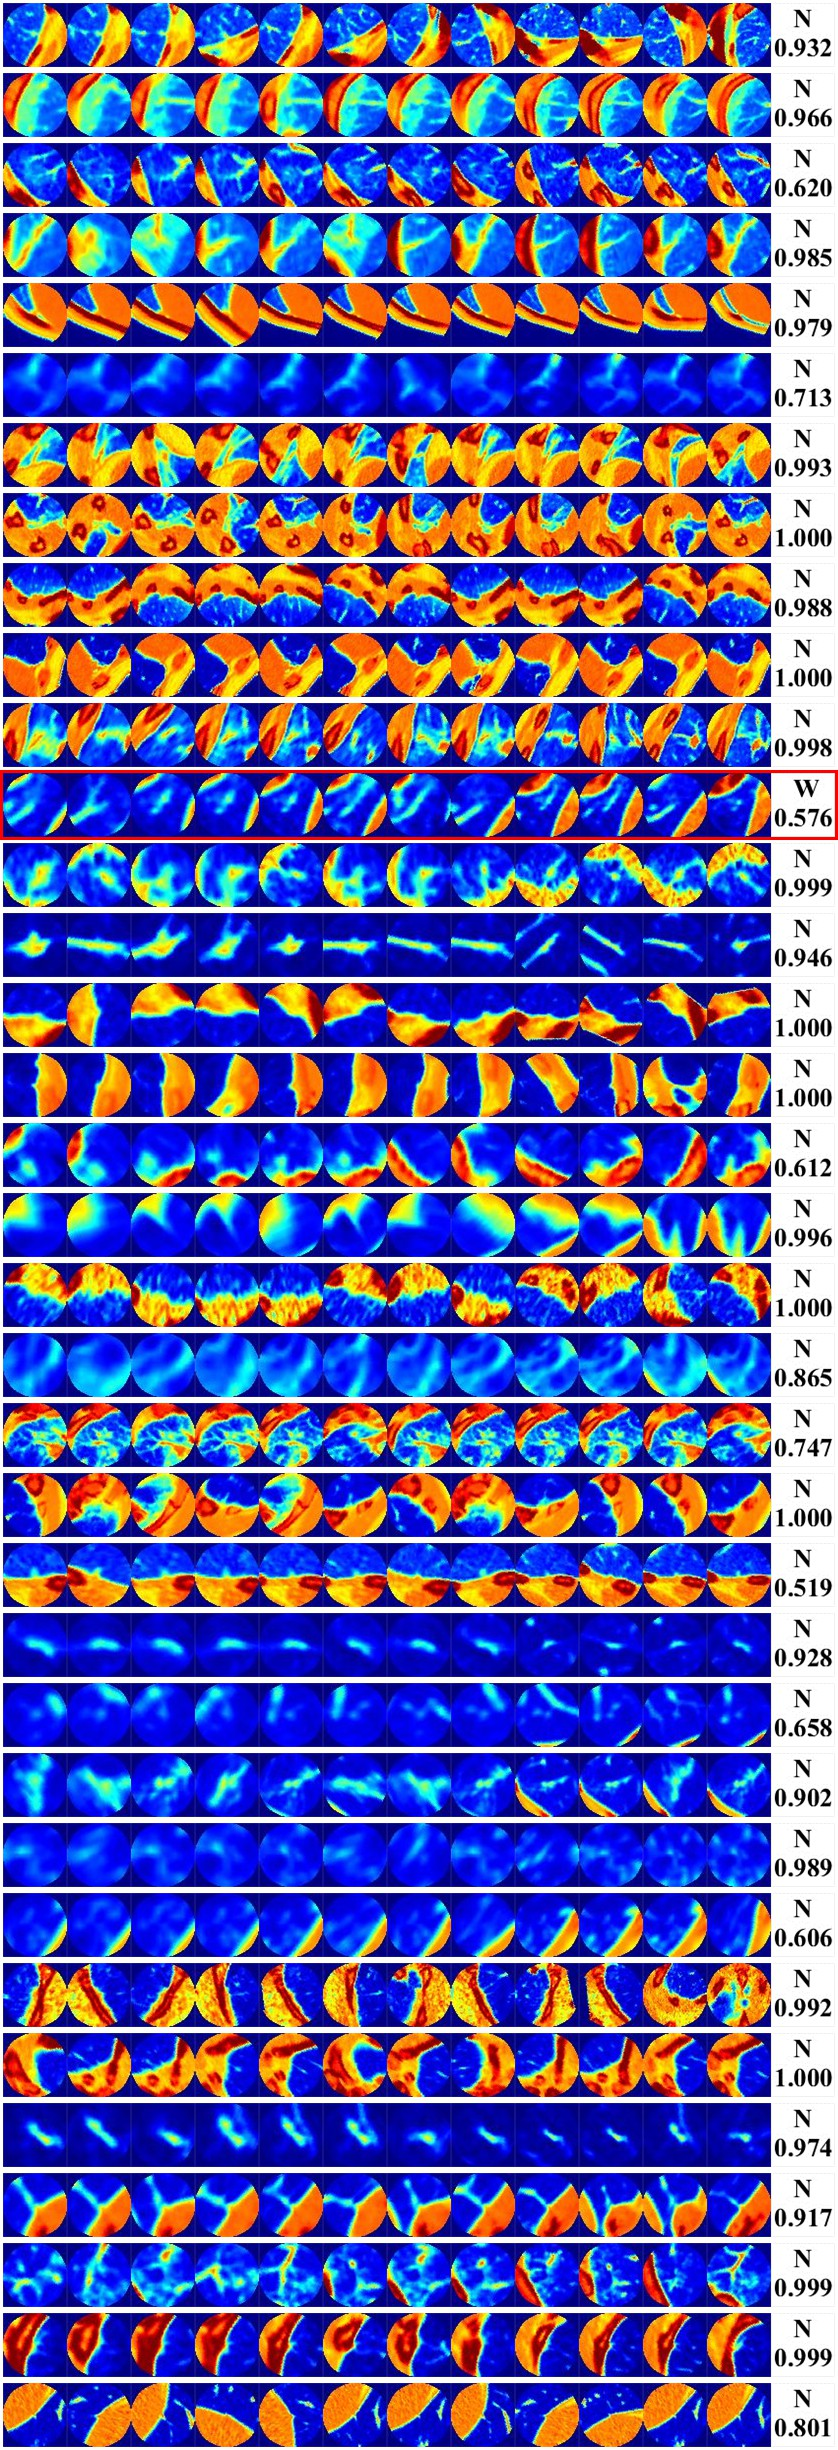
\includegraphics[width=0.45\columnwidth]{./images/lidc-msnodulecircles-nonnodule1}
}
\end{figure}
\newpage
\begin{figure}[H]
\centering
\subfigure{
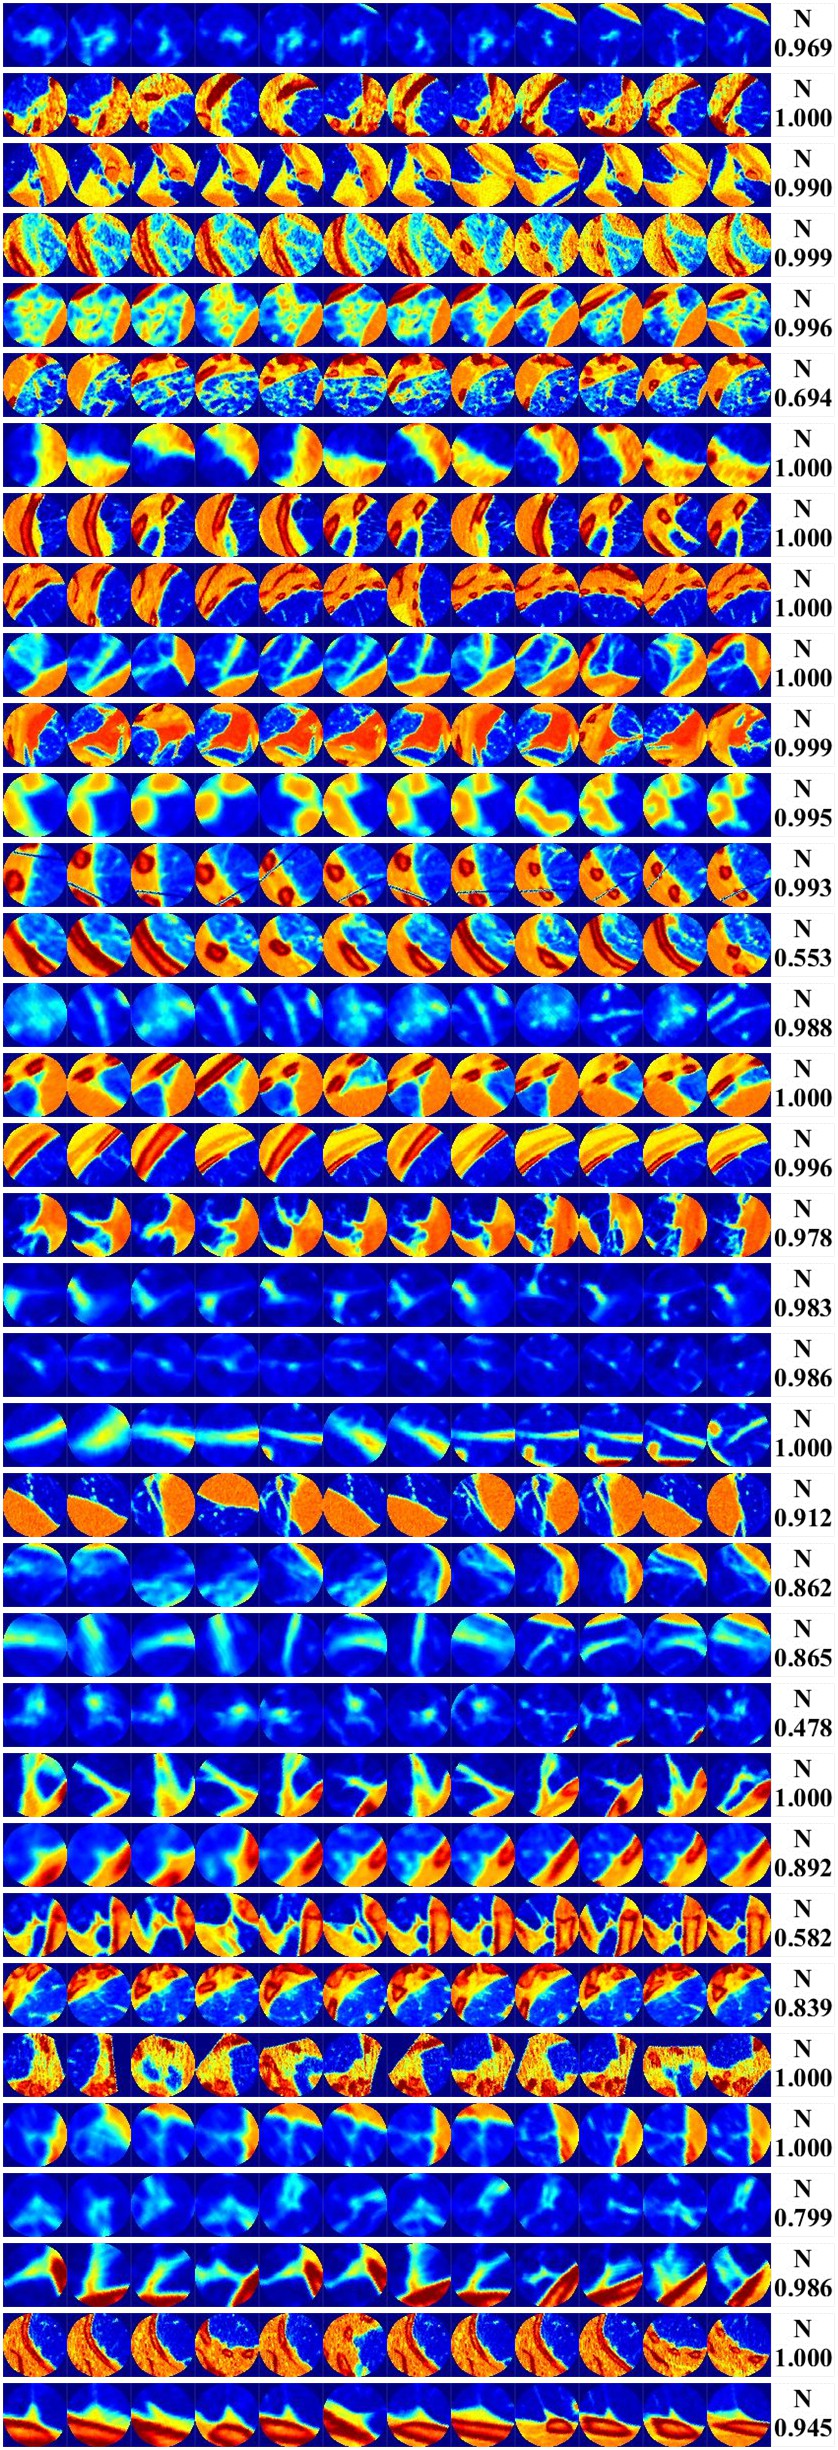
\includegraphics[width=0.45\columnwidth]{./images/lidc-msnodulecircles-nonnodule2}
}
\hspace{.1in}
\subfigure{
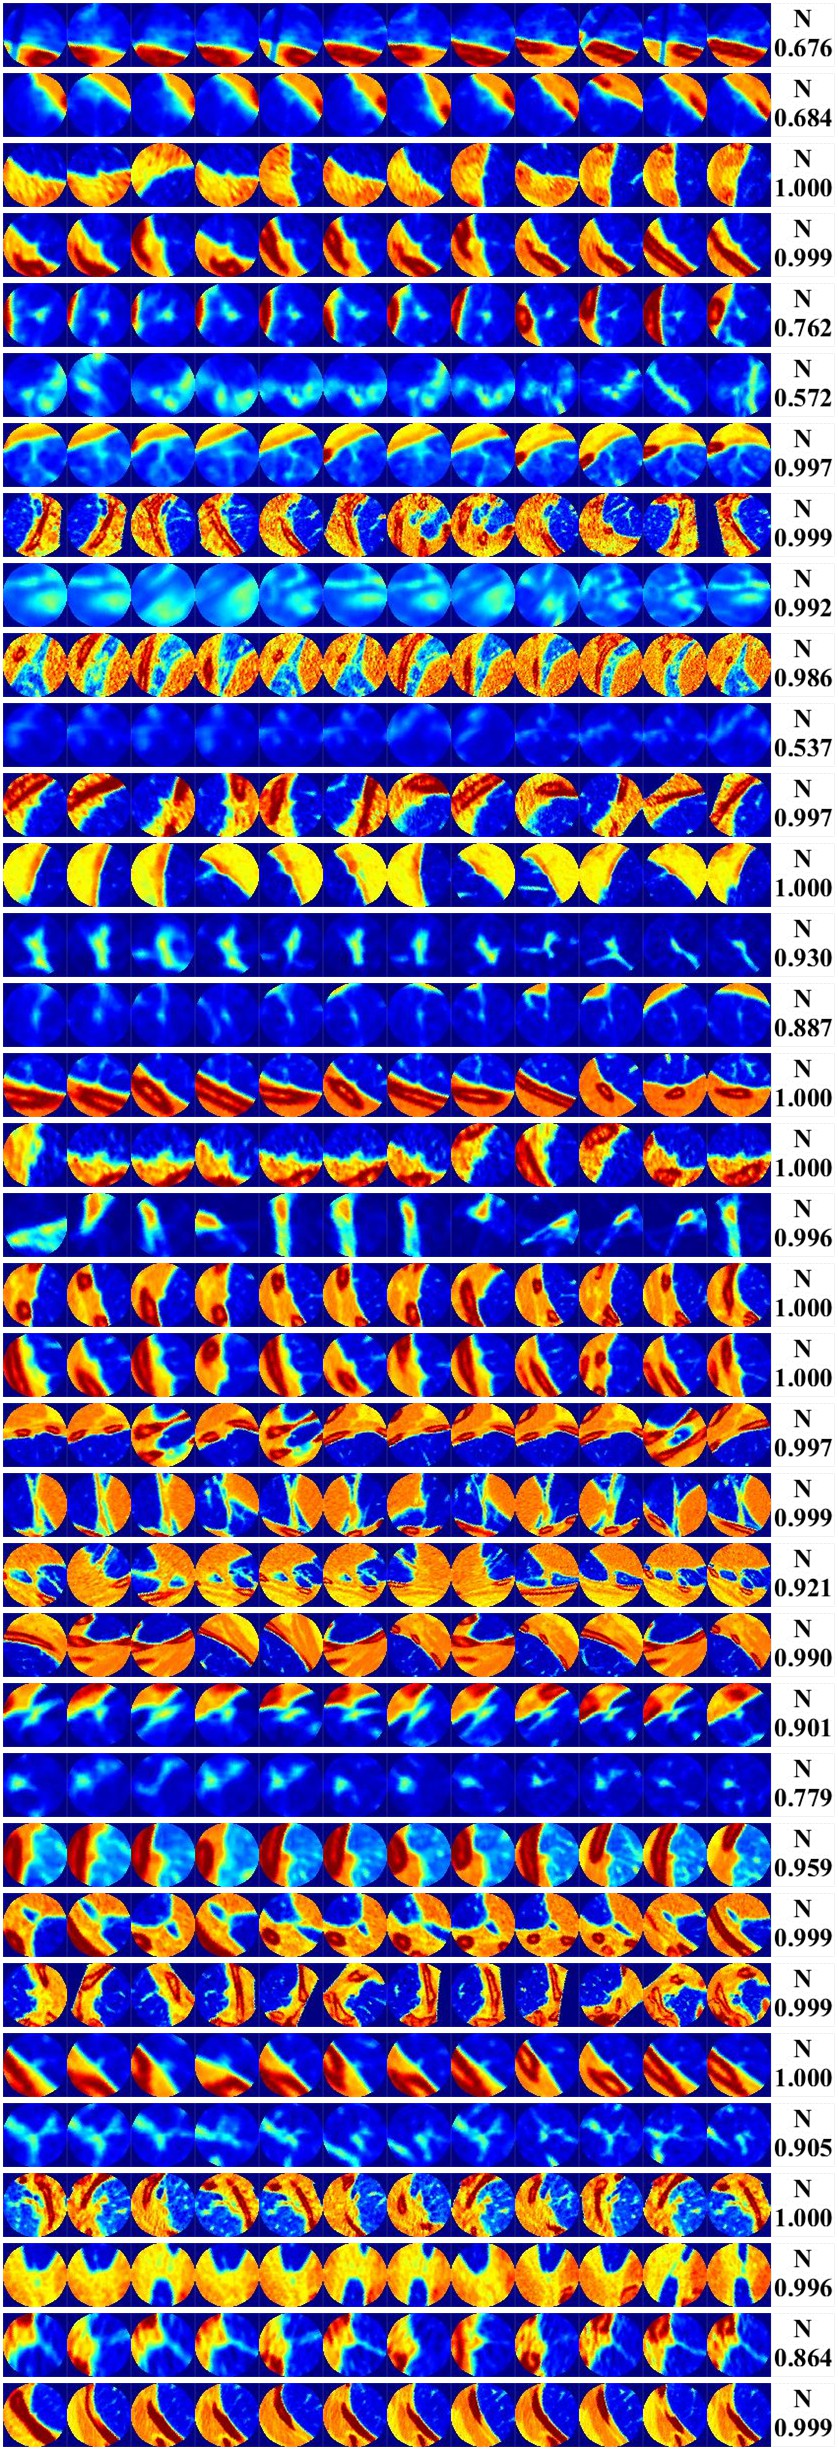
\includegraphics[width=0.45\columnwidth]{./images/lidc-msnodulecircles-nonnodule3}
}
\end{figure}
\newpage
\begin{figure}[H]
\centering
\subfigure{
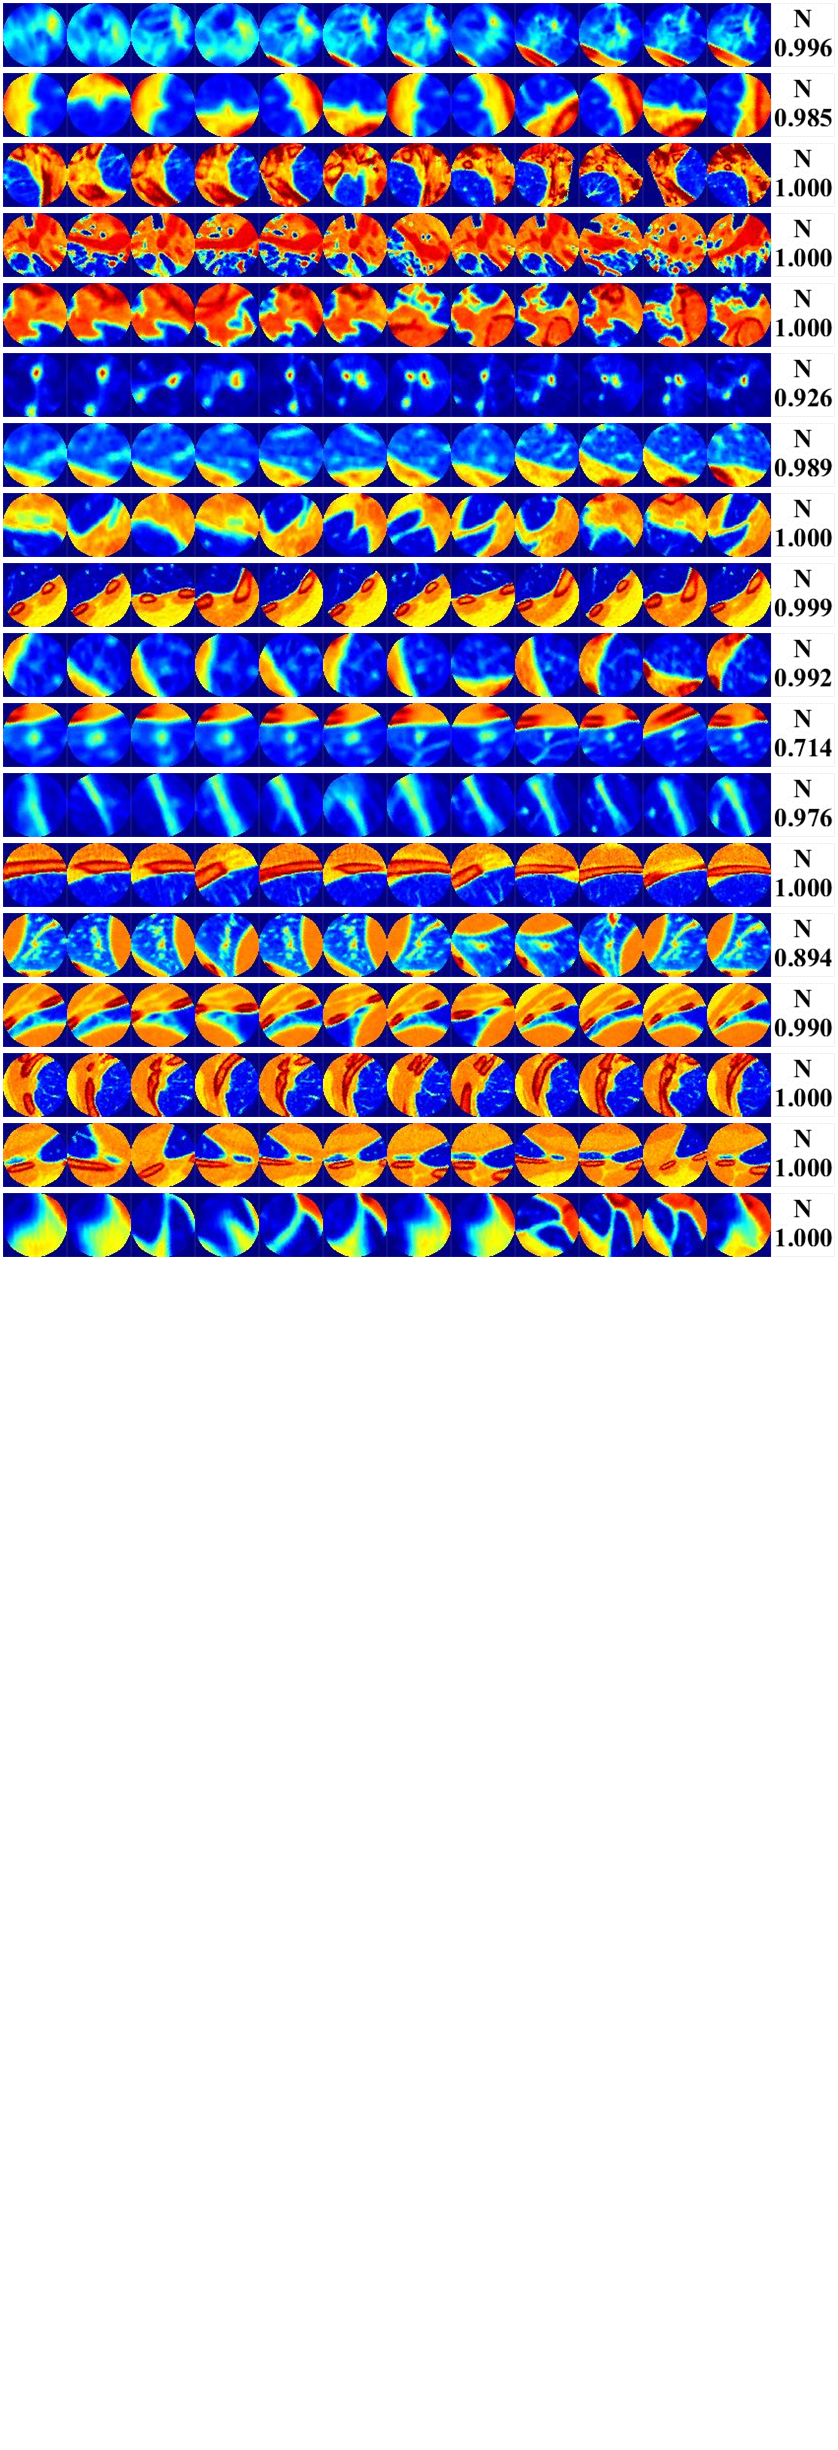
\includegraphics[width=0.45\columnwidth]{./images/lidc-msnodulecircles-nonnodule4}
}
\end{figure}

%%%%%%%%%%%%%%%%%%%%%%%%%%%%%%%%%%%%%%%%%%%%%%%%%%%%%%%%%%%%%%%%%%%%%%%%%%%%%%%%%%%
\section{\emph{ms-nodulecircles} on ELCAP}
\subsection{Overall Statistics}
The confusion matrix for each type is shown in Table~\ref{tbl:conf_cmp_elcap_nodulecircles}. The overall classification rate is 90.9\%. Results for all cases are shown. Scores are presented on the most right of the image. It should be noted that cases not correctly classified are labeled out using red rectangles.

%%%%%%%%%%%%%%%%%%%%%%%%%%%%%%%%%%
\begin{table}[H]
\caption{Confusion Matrix for \emph{ms-nodulecircles} on ELCAP}
\centering
\tabcolsep=1pt
\begin{tabular}{p{30pt}p{60pt}p{60pt}p{60pt}p{60pt}p{60pt}p{60pt}}
\toprule
\tabincell{c}{ } &\textbf{G} & \textbf{W} & \textbf{N}& \textbf{P} & \textbf{V} & \textbf{J} \\
\midrule
%%%%%%%%%%%% 666666666666666666666666666666
\rule{0pt}{10pt}
\textbf{G} & \textbf{1.00}& 0.00 & 0.00 & 0.00 & 0.00 & 0.00 \\
\rule{0pt}{10pt}
\textbf{W} & 0.00 & \textbf{0.95} & 0.05 & 0.00 & 0.00 & 0.00 \\
\rule{0pt}{10pt}
\textbf{N} & 0.04 &  0.04 &\textbf{0.92} & 0.01 & 0.00 & 0.00 \\
\rule{0pt}{10pt}
\textbf{P} & 0.02 &  0.00 &  0.06 & \textbf{0.92} & 0.00 & 0.00 \\
\rule{0pt}{10pt}
\textbf{V} & 0.05 &  0.00 &  0.02 &  0.00 & \textbf{0.93}& 0.00 \\
\rule{0pt}{10pt}
\textbf{J} & 0.04 &  0.00 &  0.20 &  0.00 & 0.00 & \textbf{0.76}\\
\bottomrule
\end{tabular}
\tabcolsep=6pt
\begin{tabular}{lll}
\rule{-3pt}{10pt}
\tabincell{l}{G = \underline{G}round glass optic} & \tabincell{l}{W = \underline{W}ell-circumscribed} & \tabincell{c}{N = \underline{N}on-nodule} \\
\tabincell{l}{P = \underline{P}leural-tail} & \tabincell{l}{V = \underline{V}ascularized} & \tabincell{l}{J = \underline{J}uxta-pleural} \\
\end{tabular}
\label{tbl:conf_cmp_elcap_nodulecircles}
\end{table}

\subsection{Results}
See following pages.

%%%%%%%%%%%%%%%%%%%%%%%%%%%%%%%%%%%%%%%%%%%%%%%%%%%%%%%%%%%%%%%%%%%%%
\newpage
\subsection{Well-circumscribed for \emph{ms-nodulecircles}}
\begin{figure}[H]
 \centering
\subfigure{
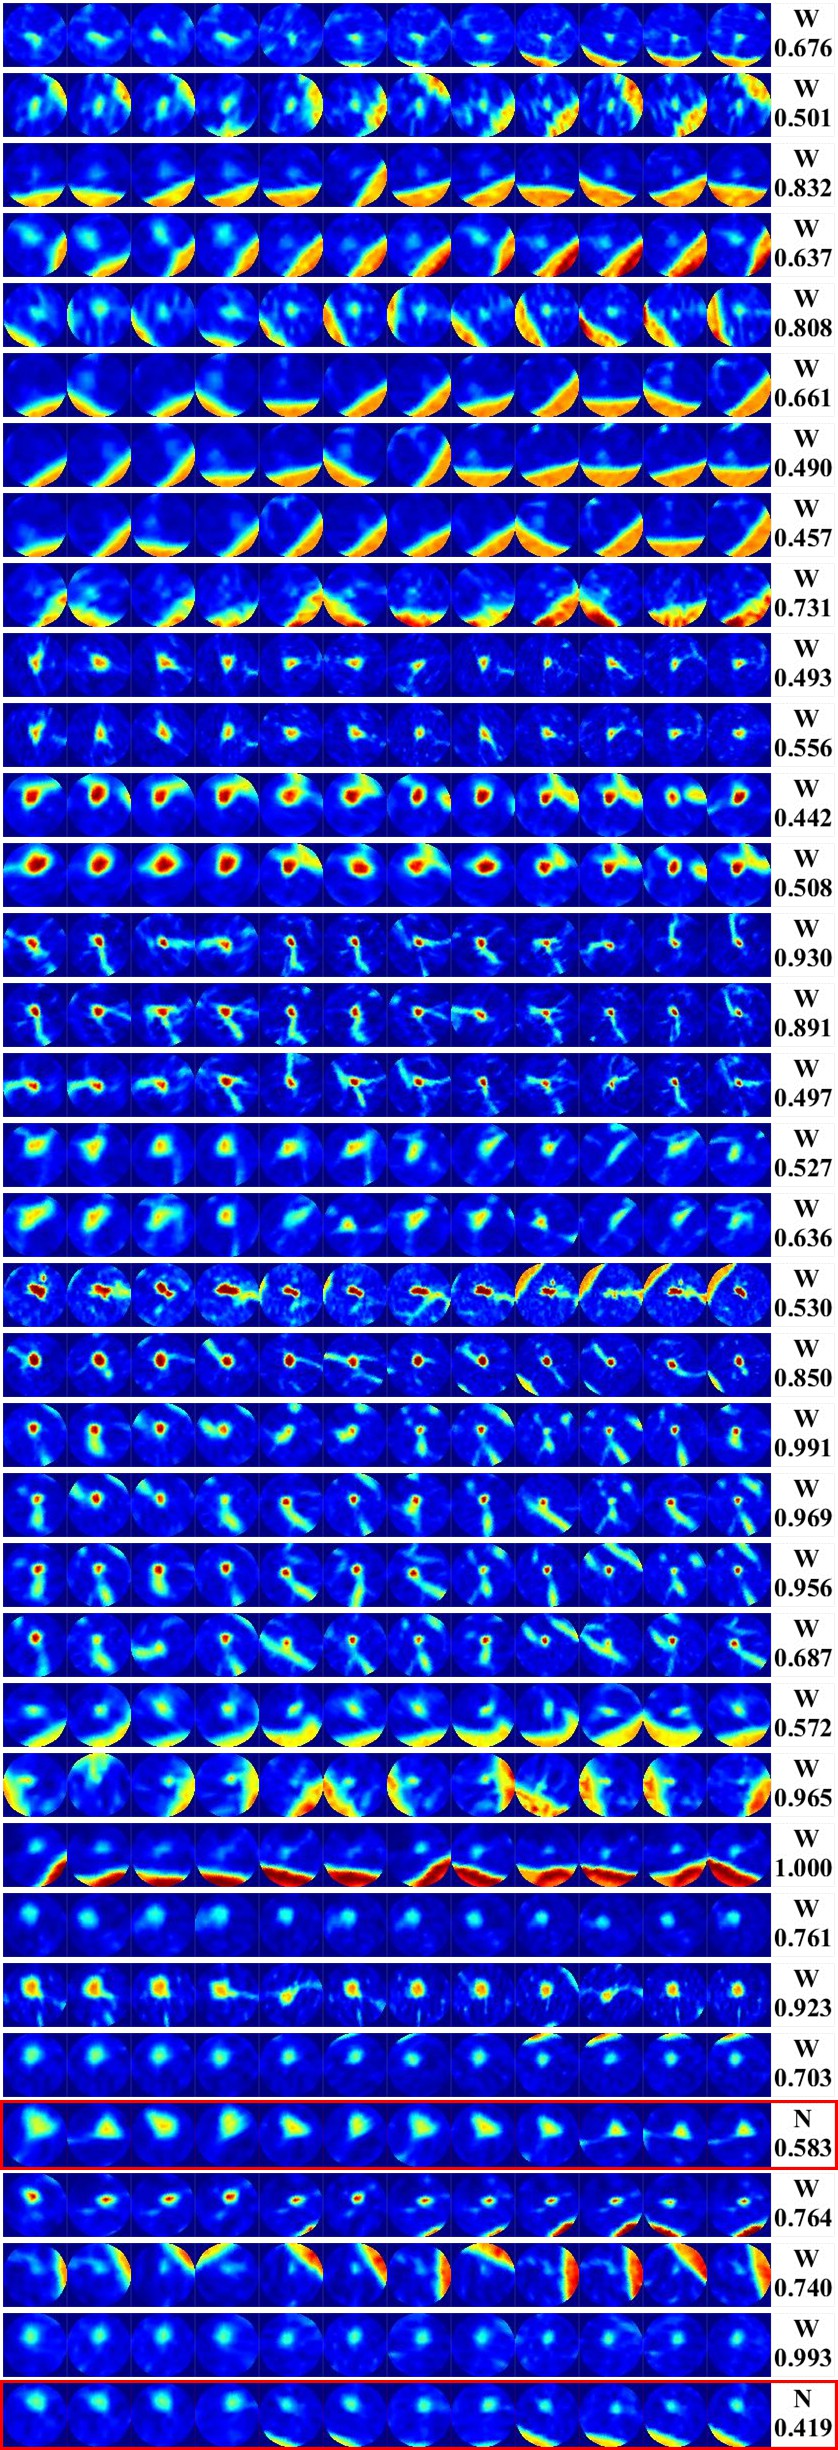
\includegraphics[width=0.45\columnwidth]{./images/elcap-msnodulecircles-iso0}
}
\hspace{.1in}
\subfigure{
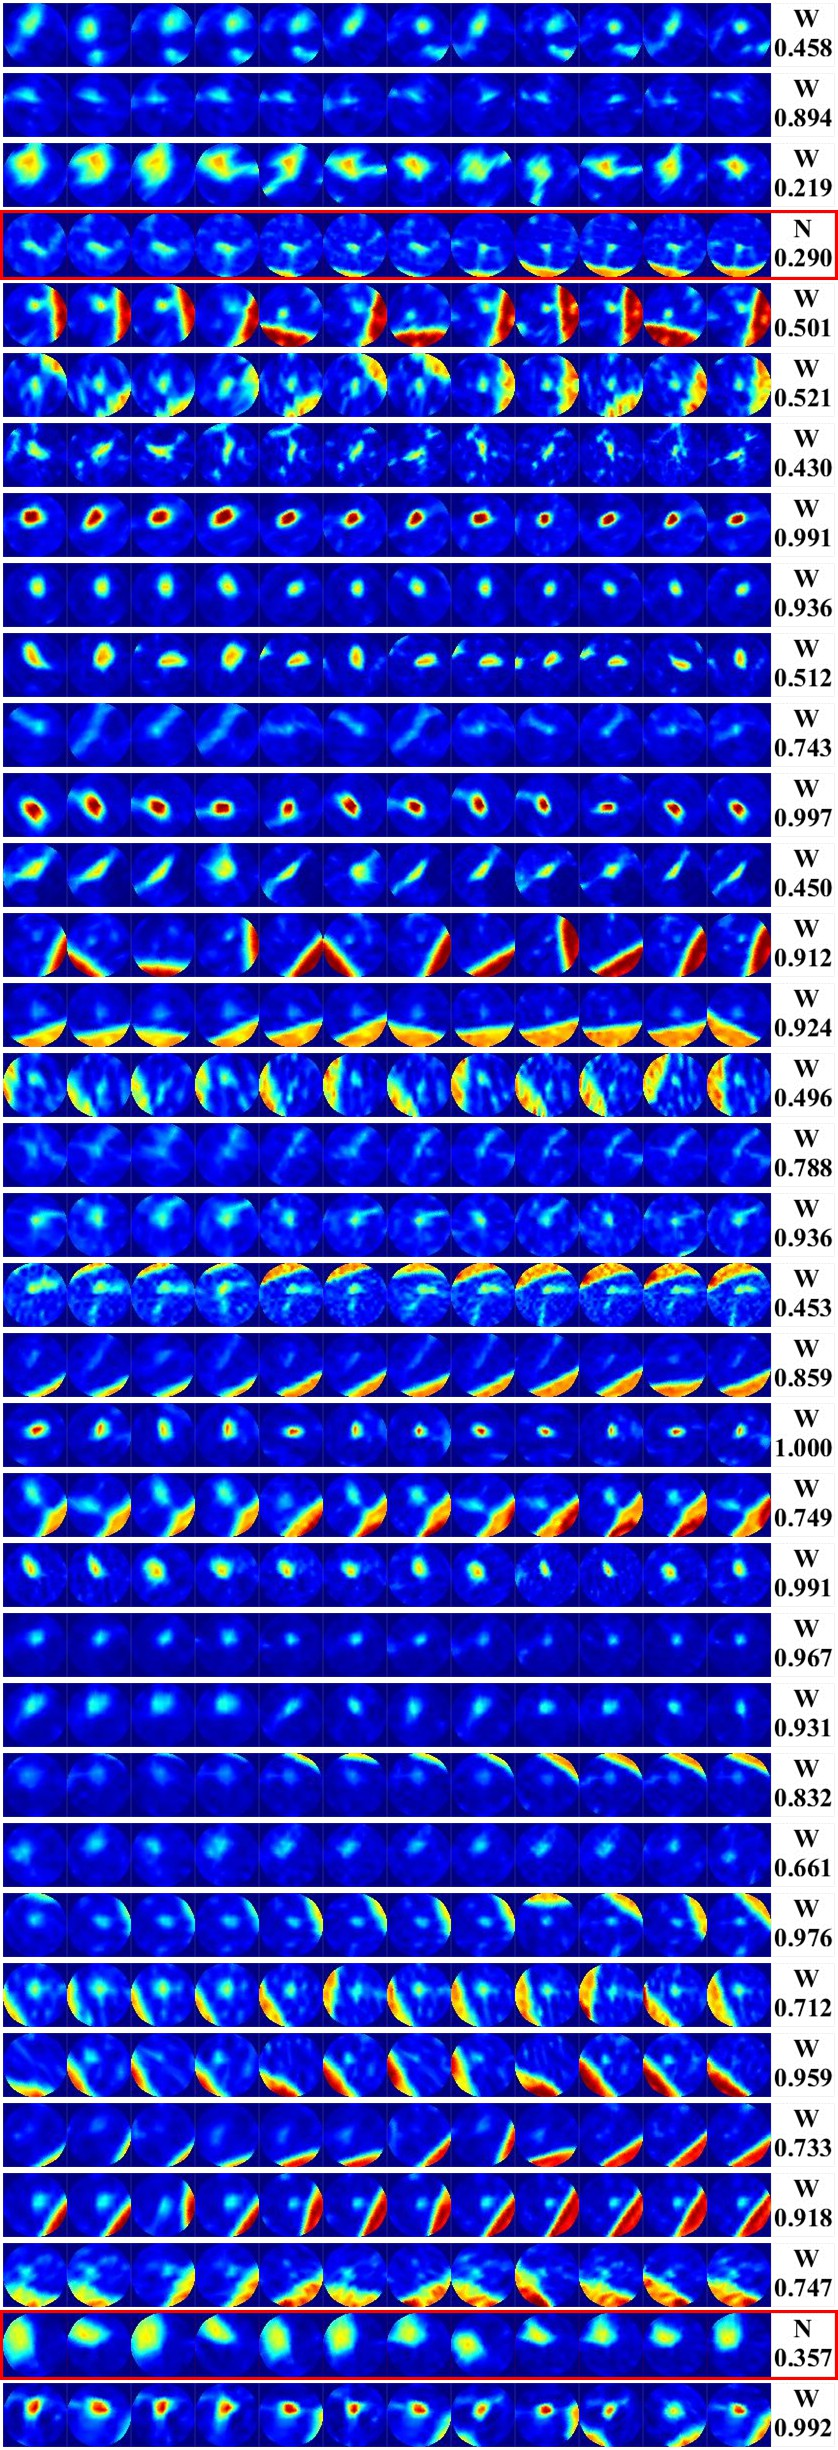
\includegraphics[width=0.45\columnwidth]{./images/elcap-msnodulecircles-iso1}
}
\end{figure}

\newpage
\begin{figure}[H]
\centering
\subfigure{
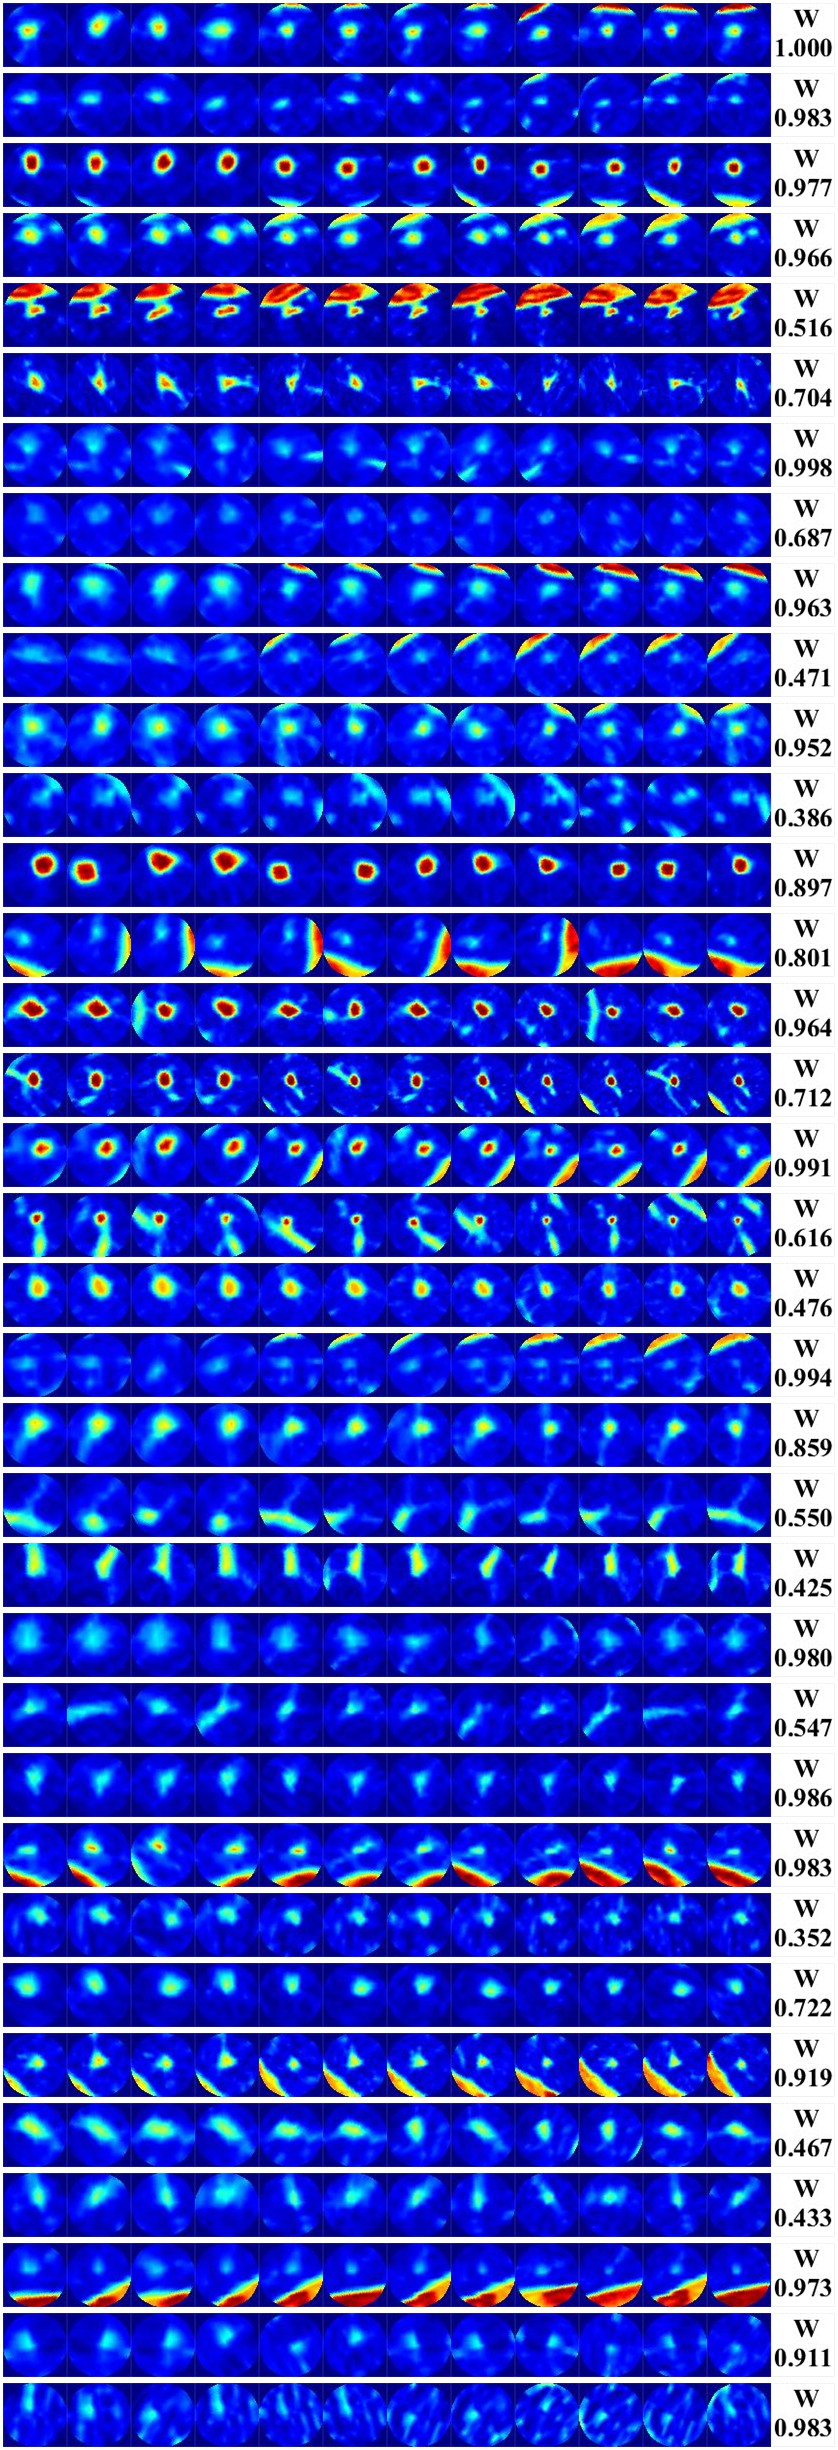
\includegraphics[width=0.45\columnwidth]{./images/elcap-msnodulecircles-iso2}
}
\hspace{.1in}
\subfigure{
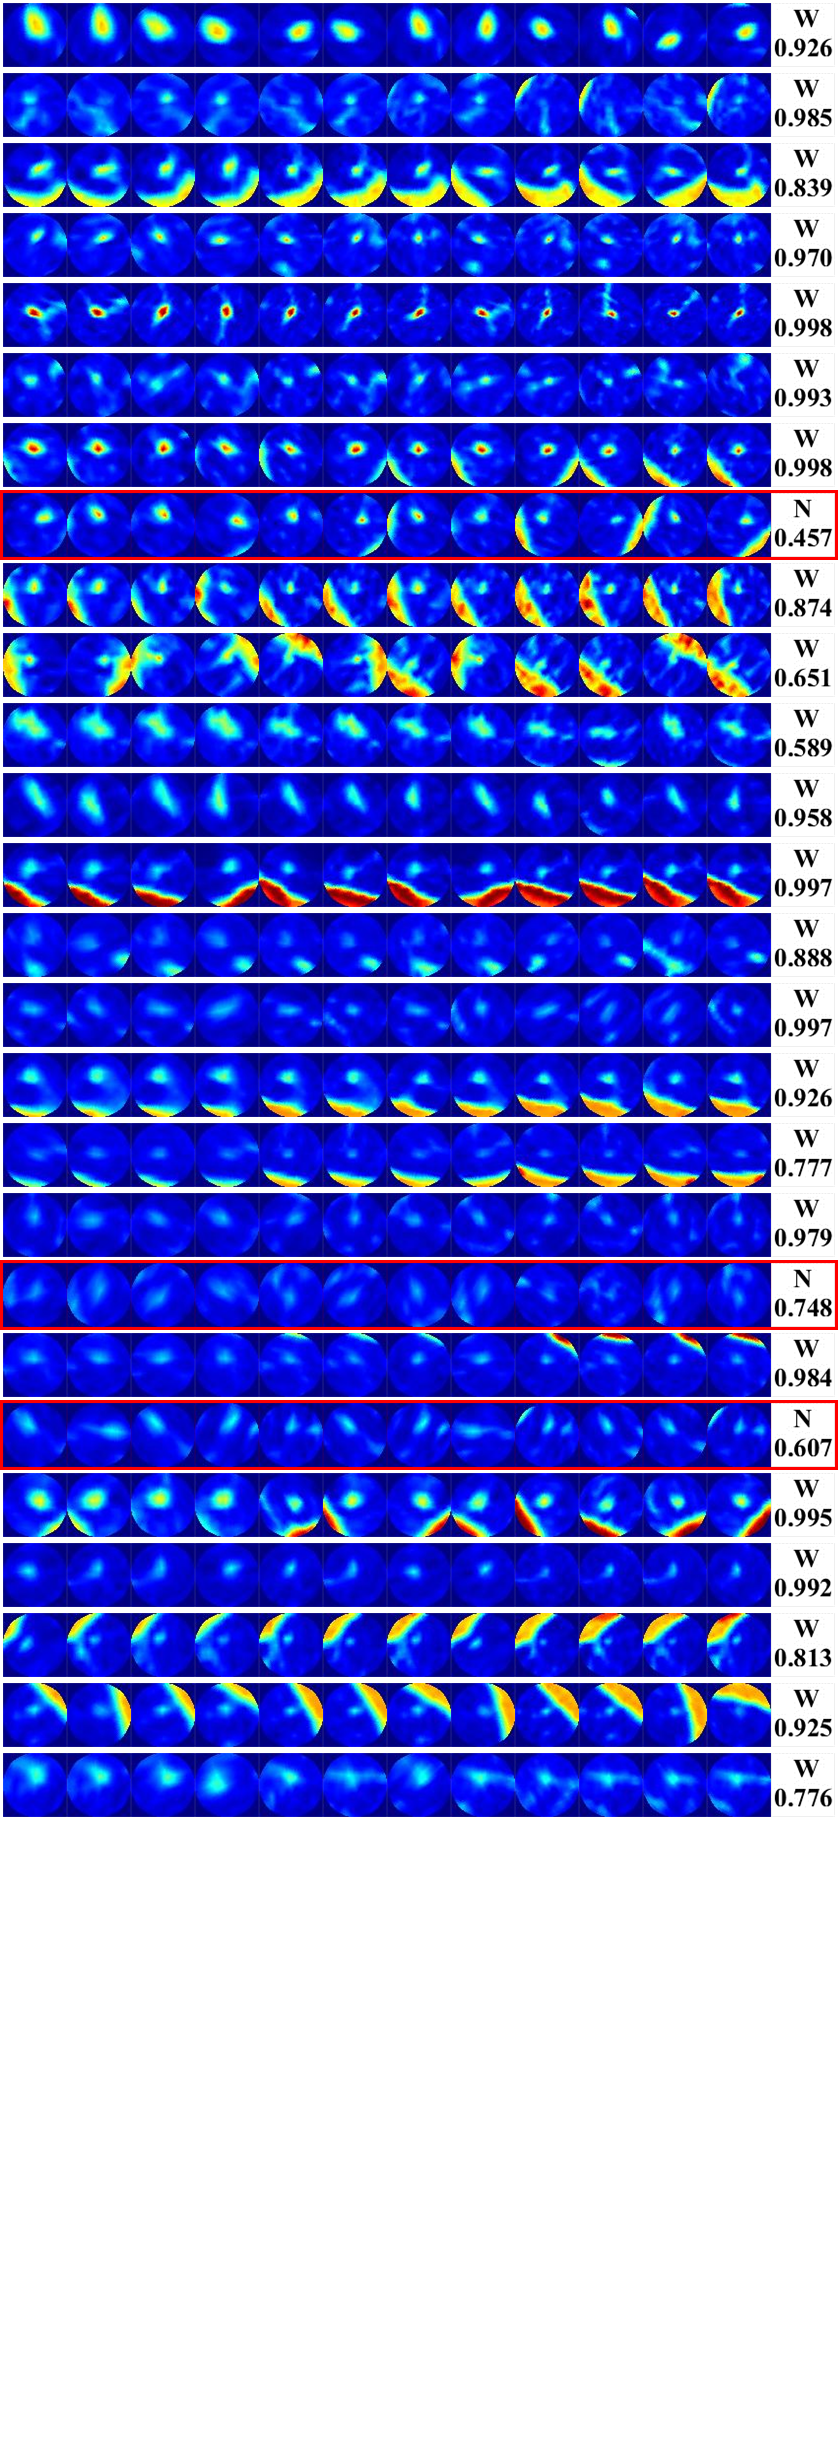
\includegraphics[width=0.45\columnwidth]{./images/elcap-msnodulecircles-iso3}
}
\end{figure}

\newpage
\subsection{GGO for \emph{ms-nodulecircles}}
\begin{figure}[H]
\centering
\subfigure{
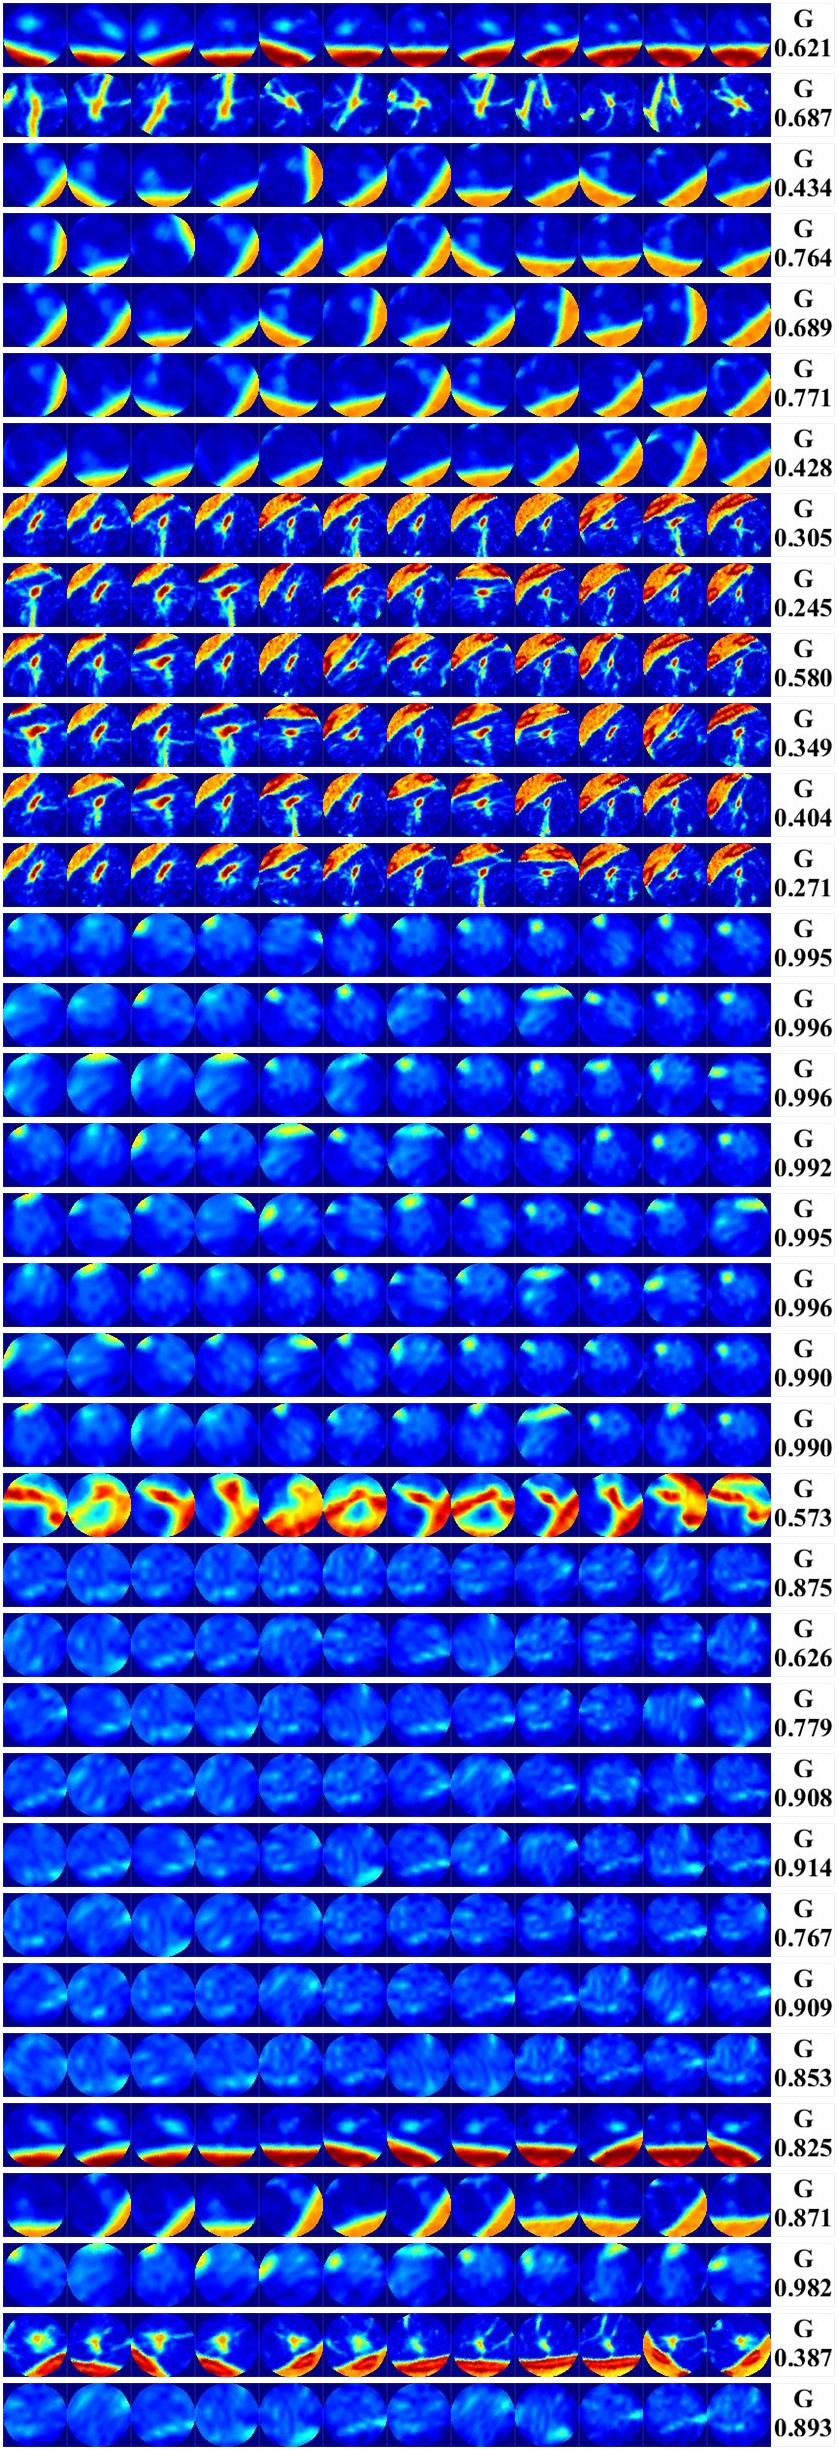
\includegraphics[width=0.45\columnwidth]{./images/elcap-msnodulecircles-ggo0}
}
\hspace{.1in}
\subfigure{
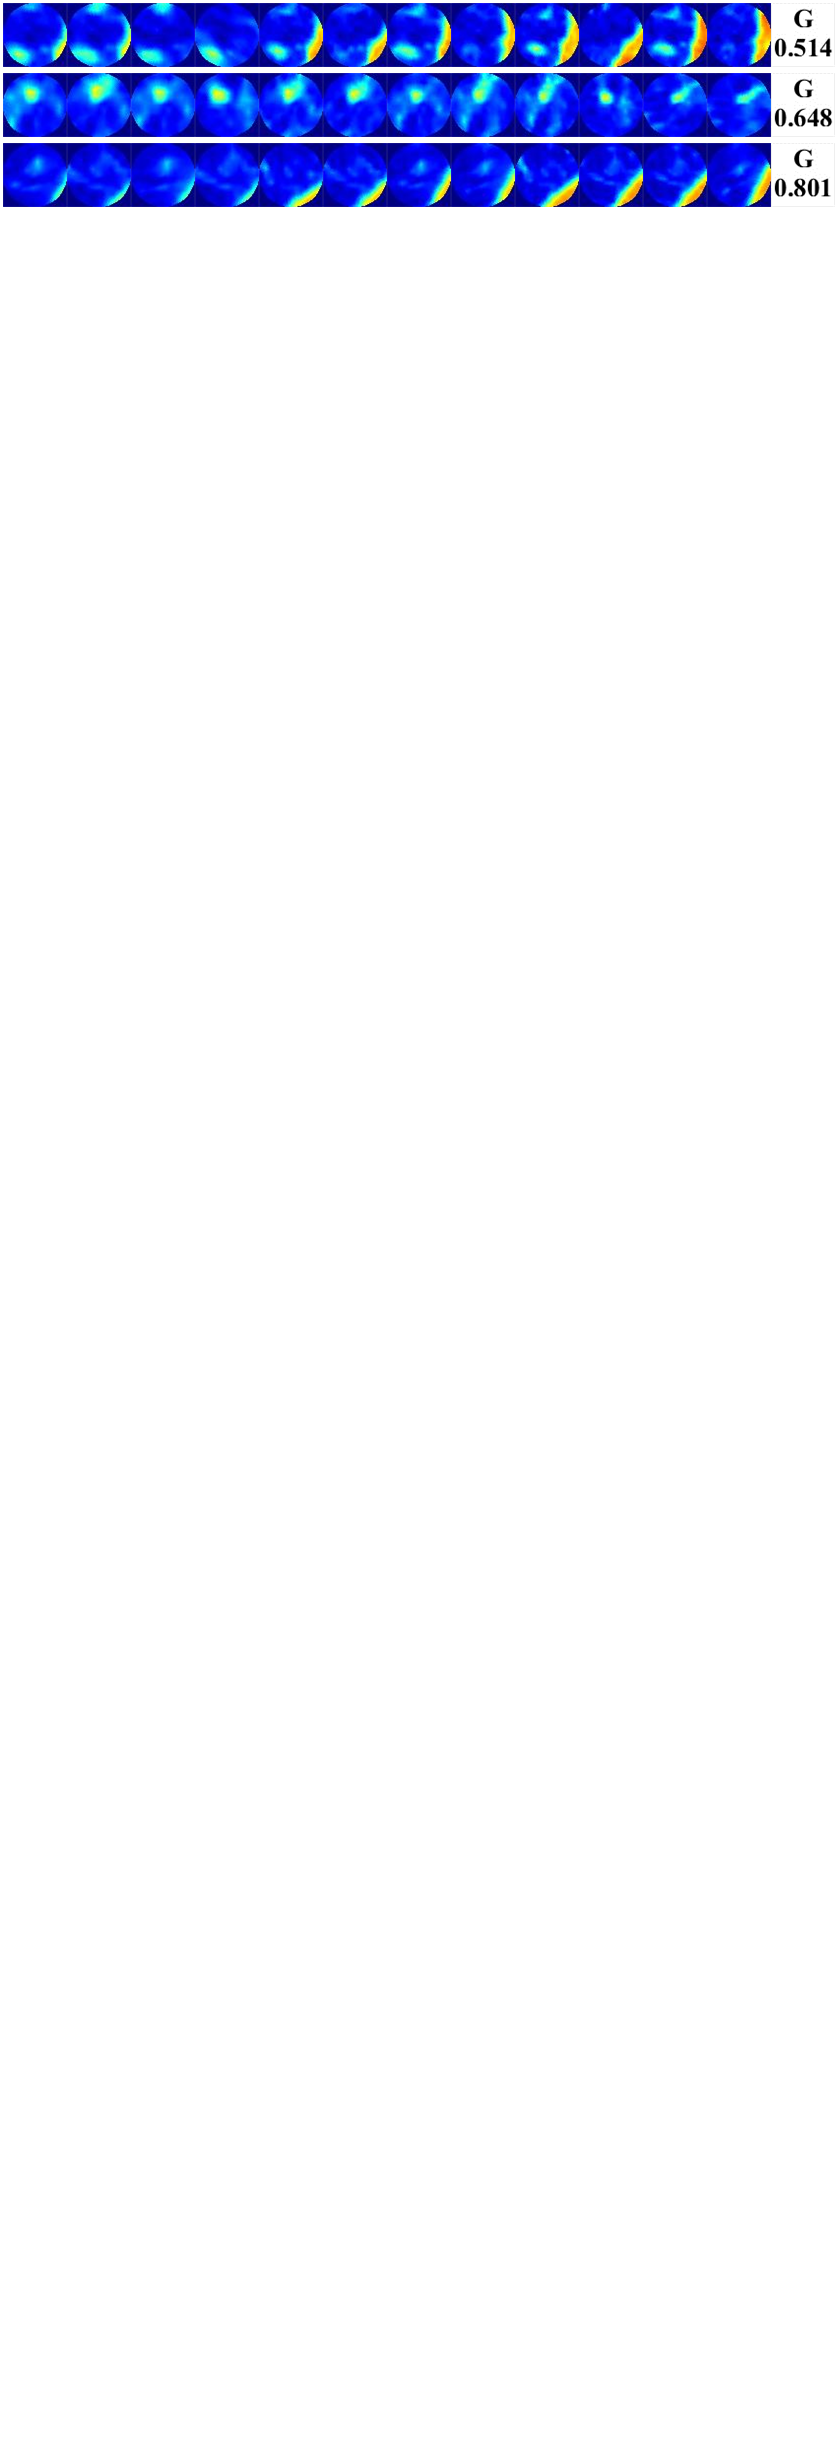
\includegraphics[width=0.45\columnwidth]{./images/elcap-msnodulecircles-ggo1}
}
\end{figure}

\newpage
\subsection{Juxta-pleural for \emph{ms-nodulecircles}}
\begin{figure}[H]
\centering
\subfigure{
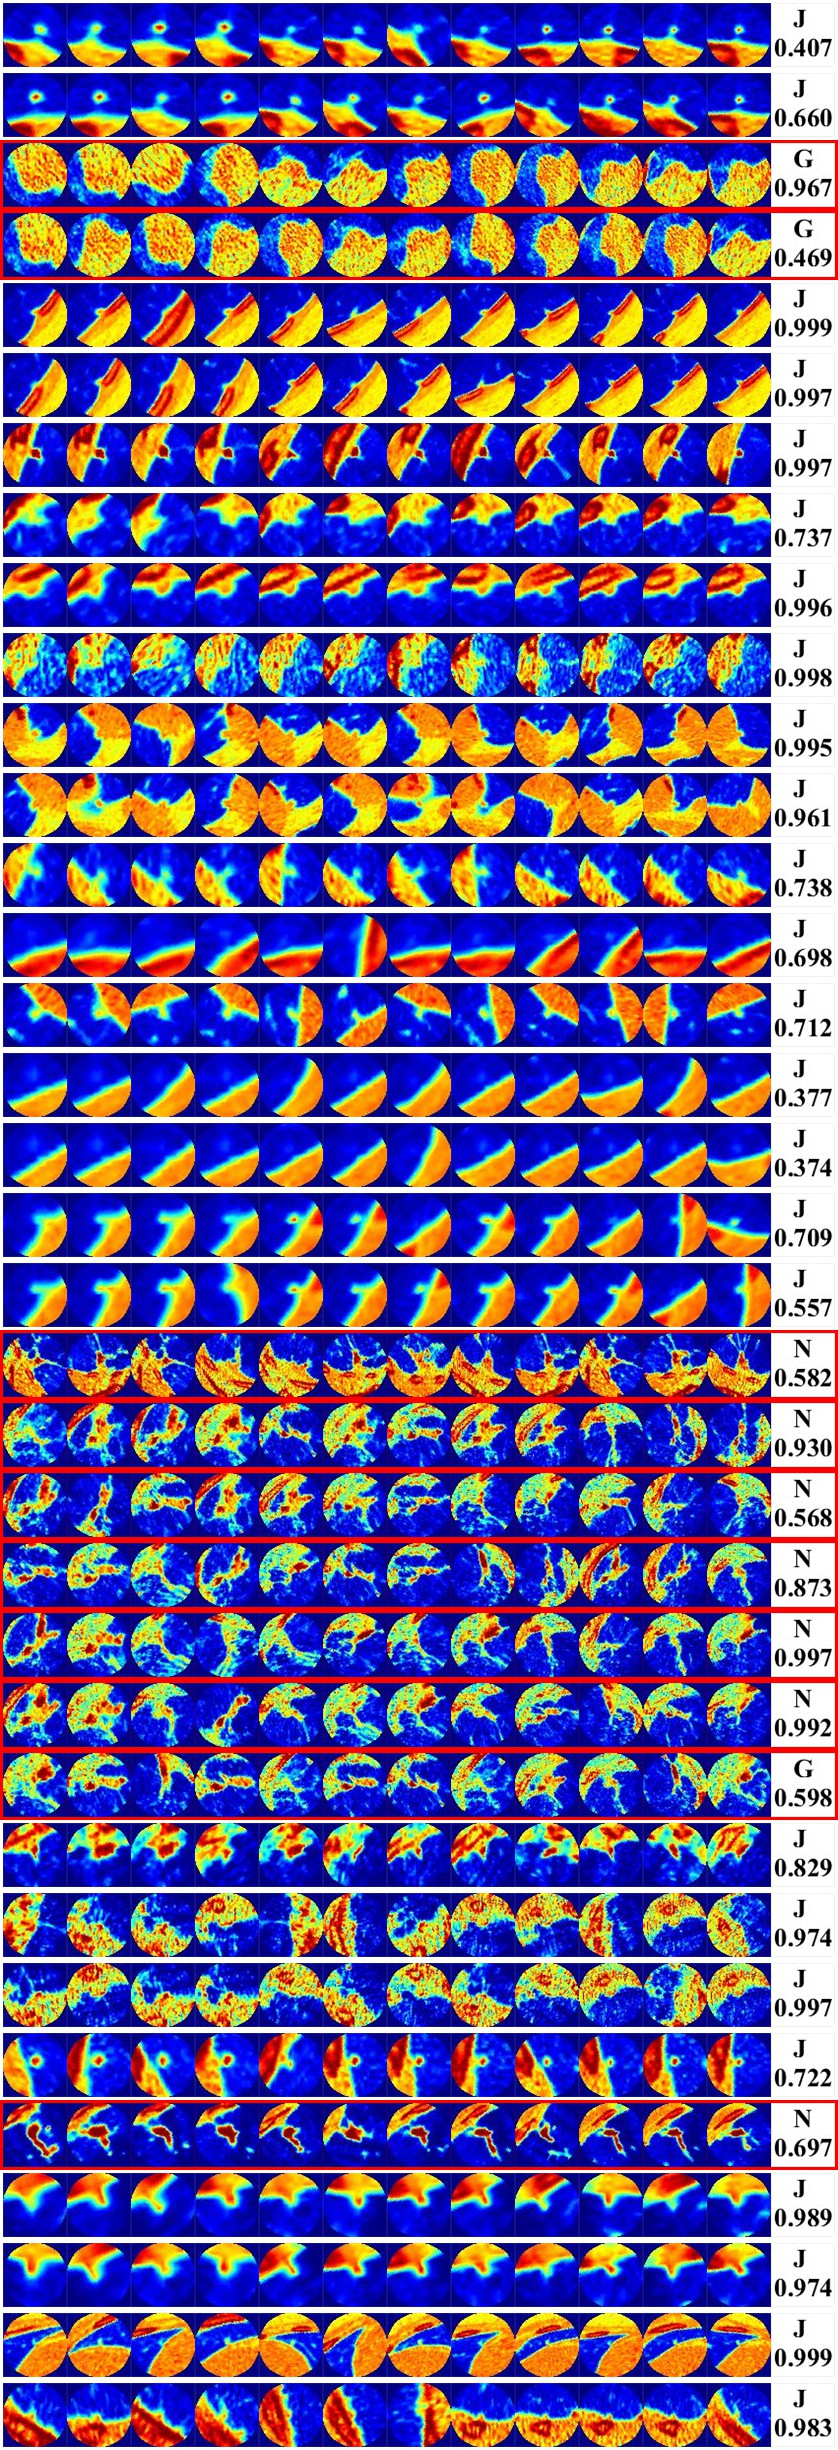
\includegraphics[width=0.45\columnwidth]{./images/elcap-msnodulecircles-wall0}
}
\hspace{.1in}
\subfigure{
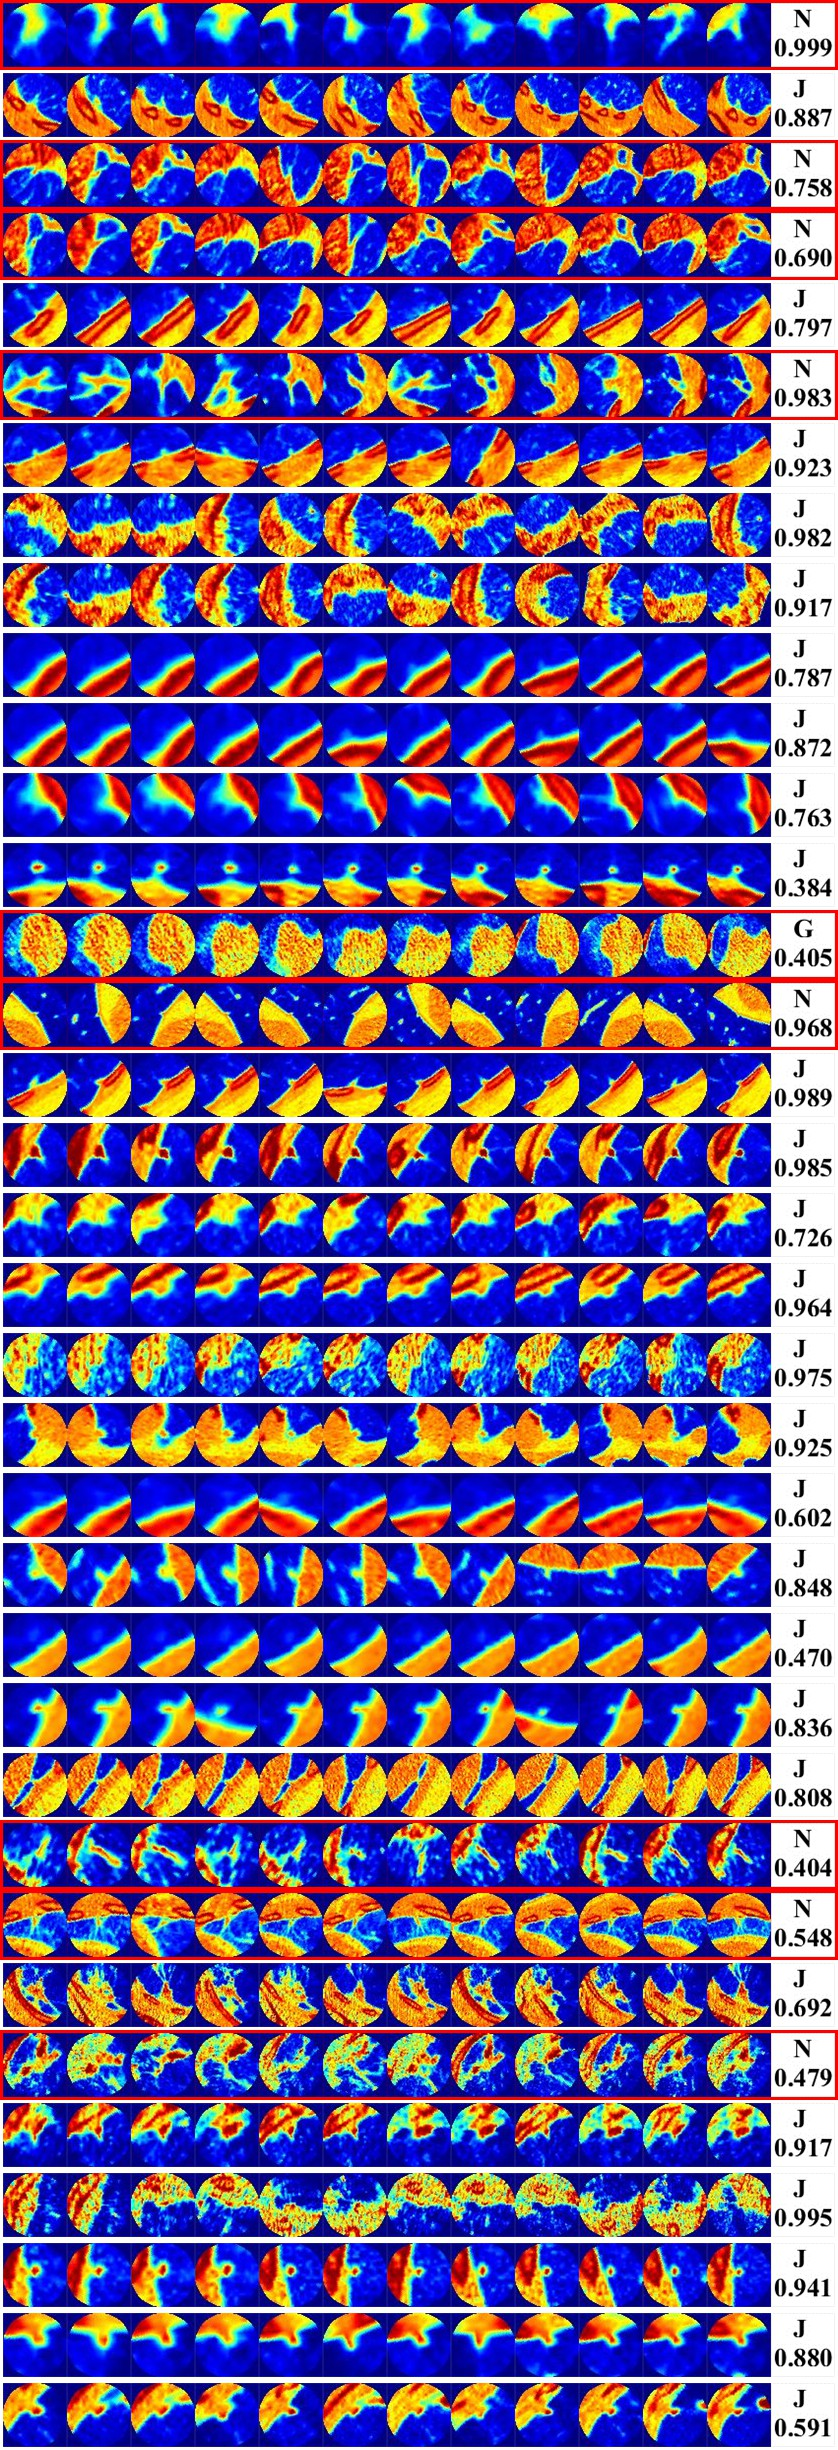
\includegraphics[width=0.45\columnwidth]{./images/elcap-msnodulecircles-wall1}
}
\end{figure}
\newpage
\begin{figure}[H]
\centering
\subfigure{
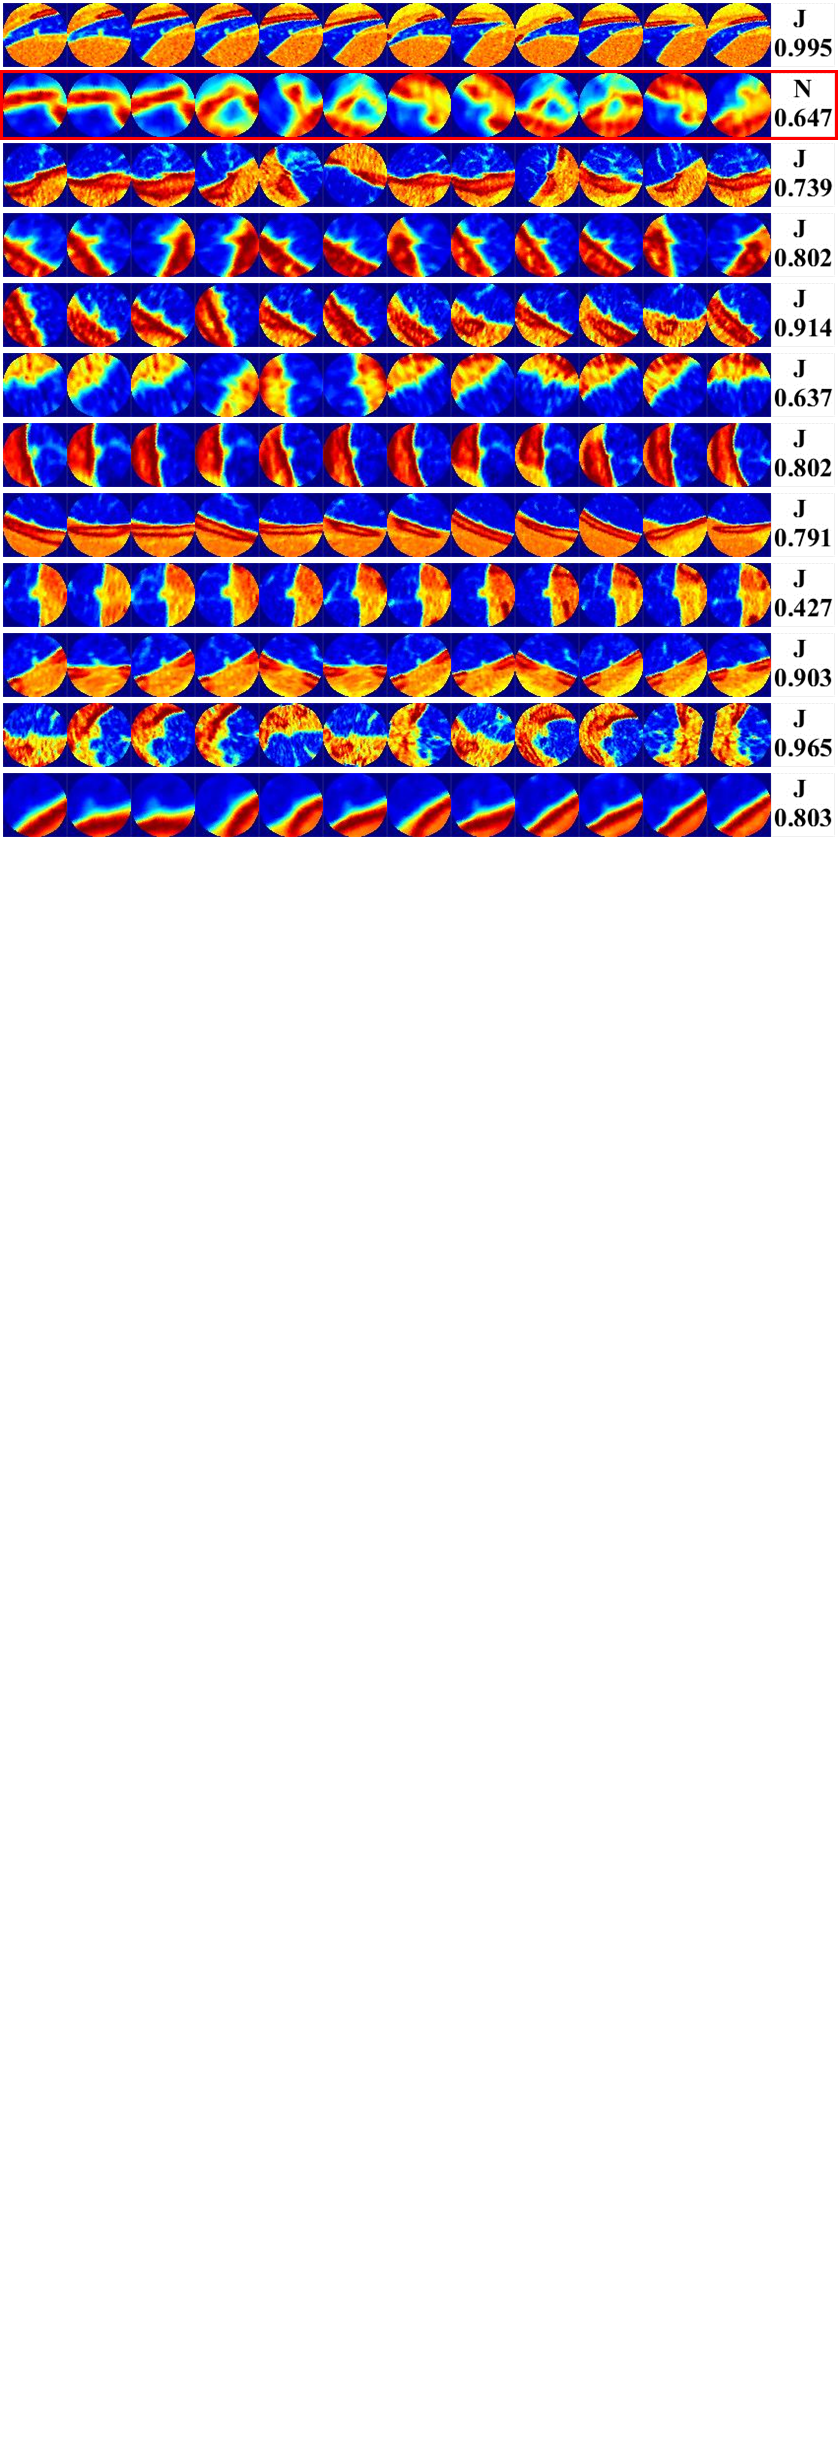
\includegraphics[width=0.45\columnwidth]{./images/elcap-msnodulecircles-wall2}
}
\end{figure}

\newpage
\subsection{Pleural-tail for \emph{ms-nodulecircles}}
\begin{figure}[H]
\centering
\subfigure{
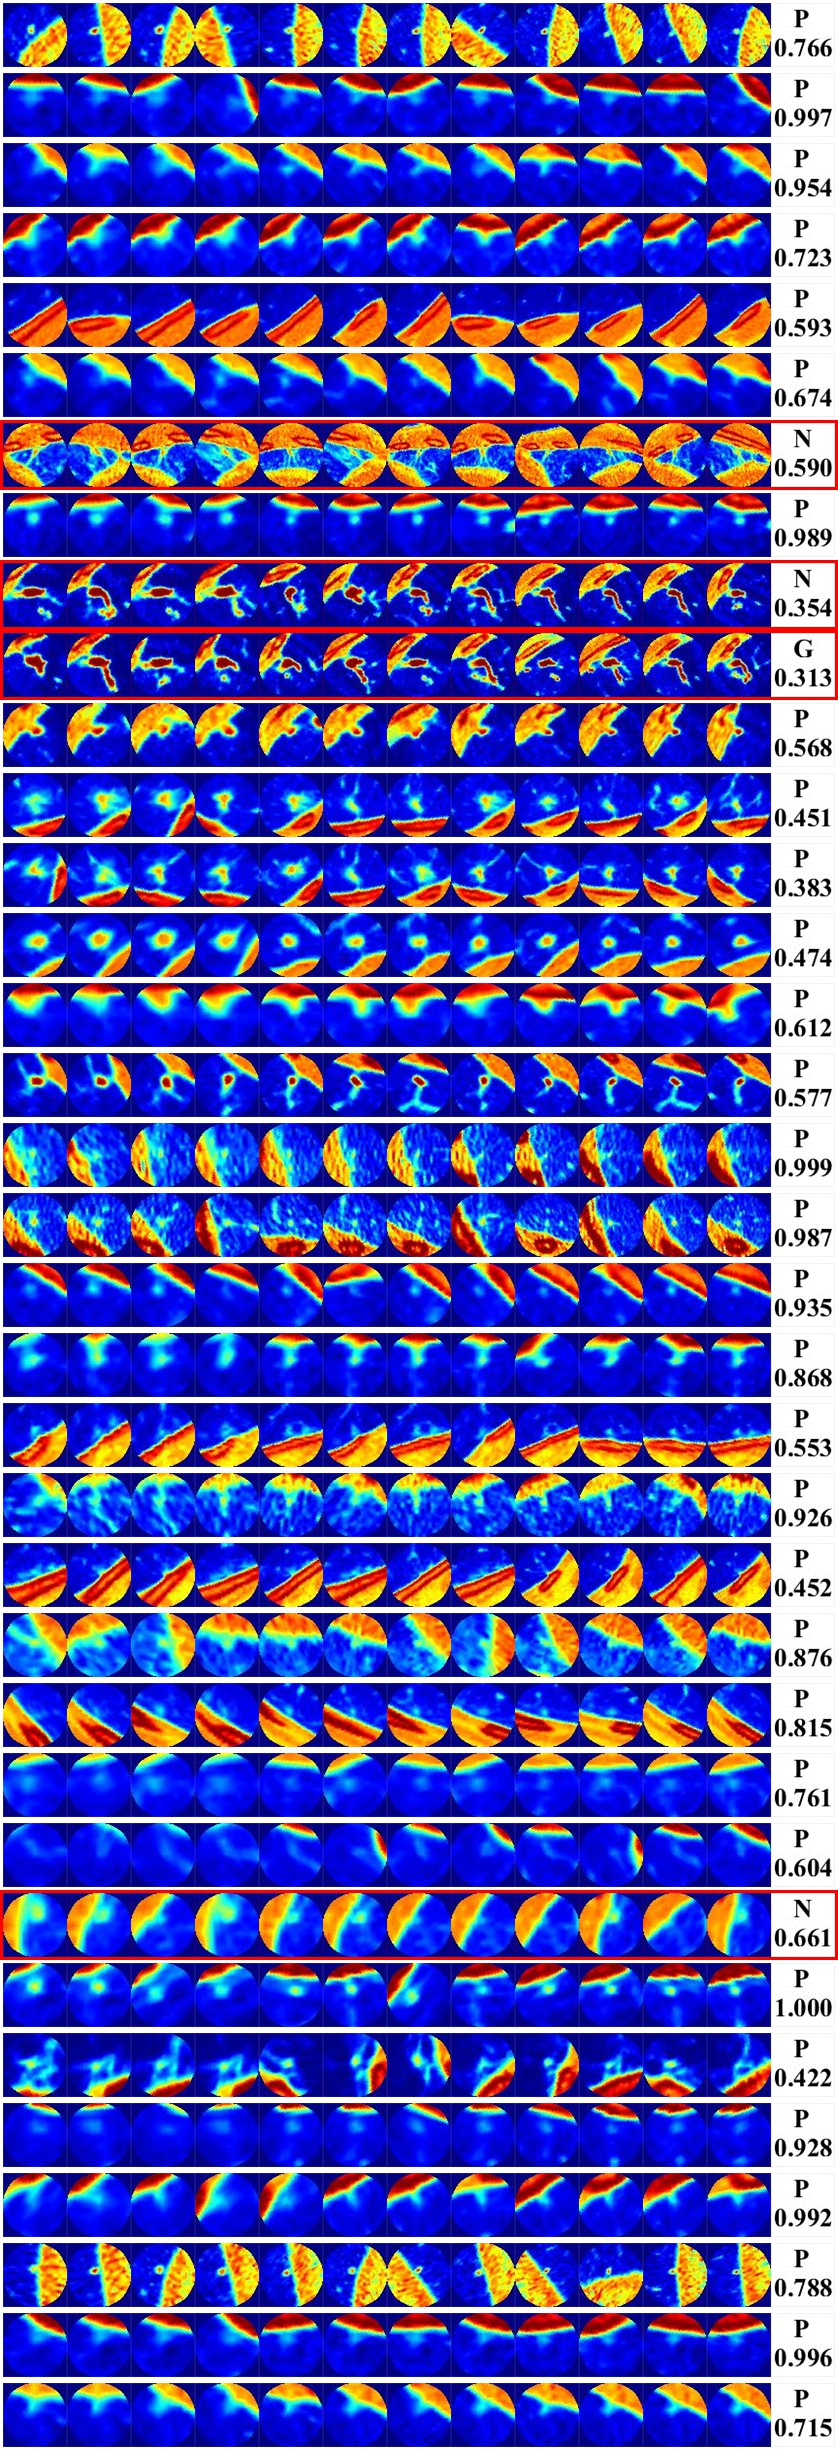
\includegraphics[width=0.45\columnwidth]{./images/elcap-msnodulecircles-tail0}
}
\hspace{.1in}
\subfigure{
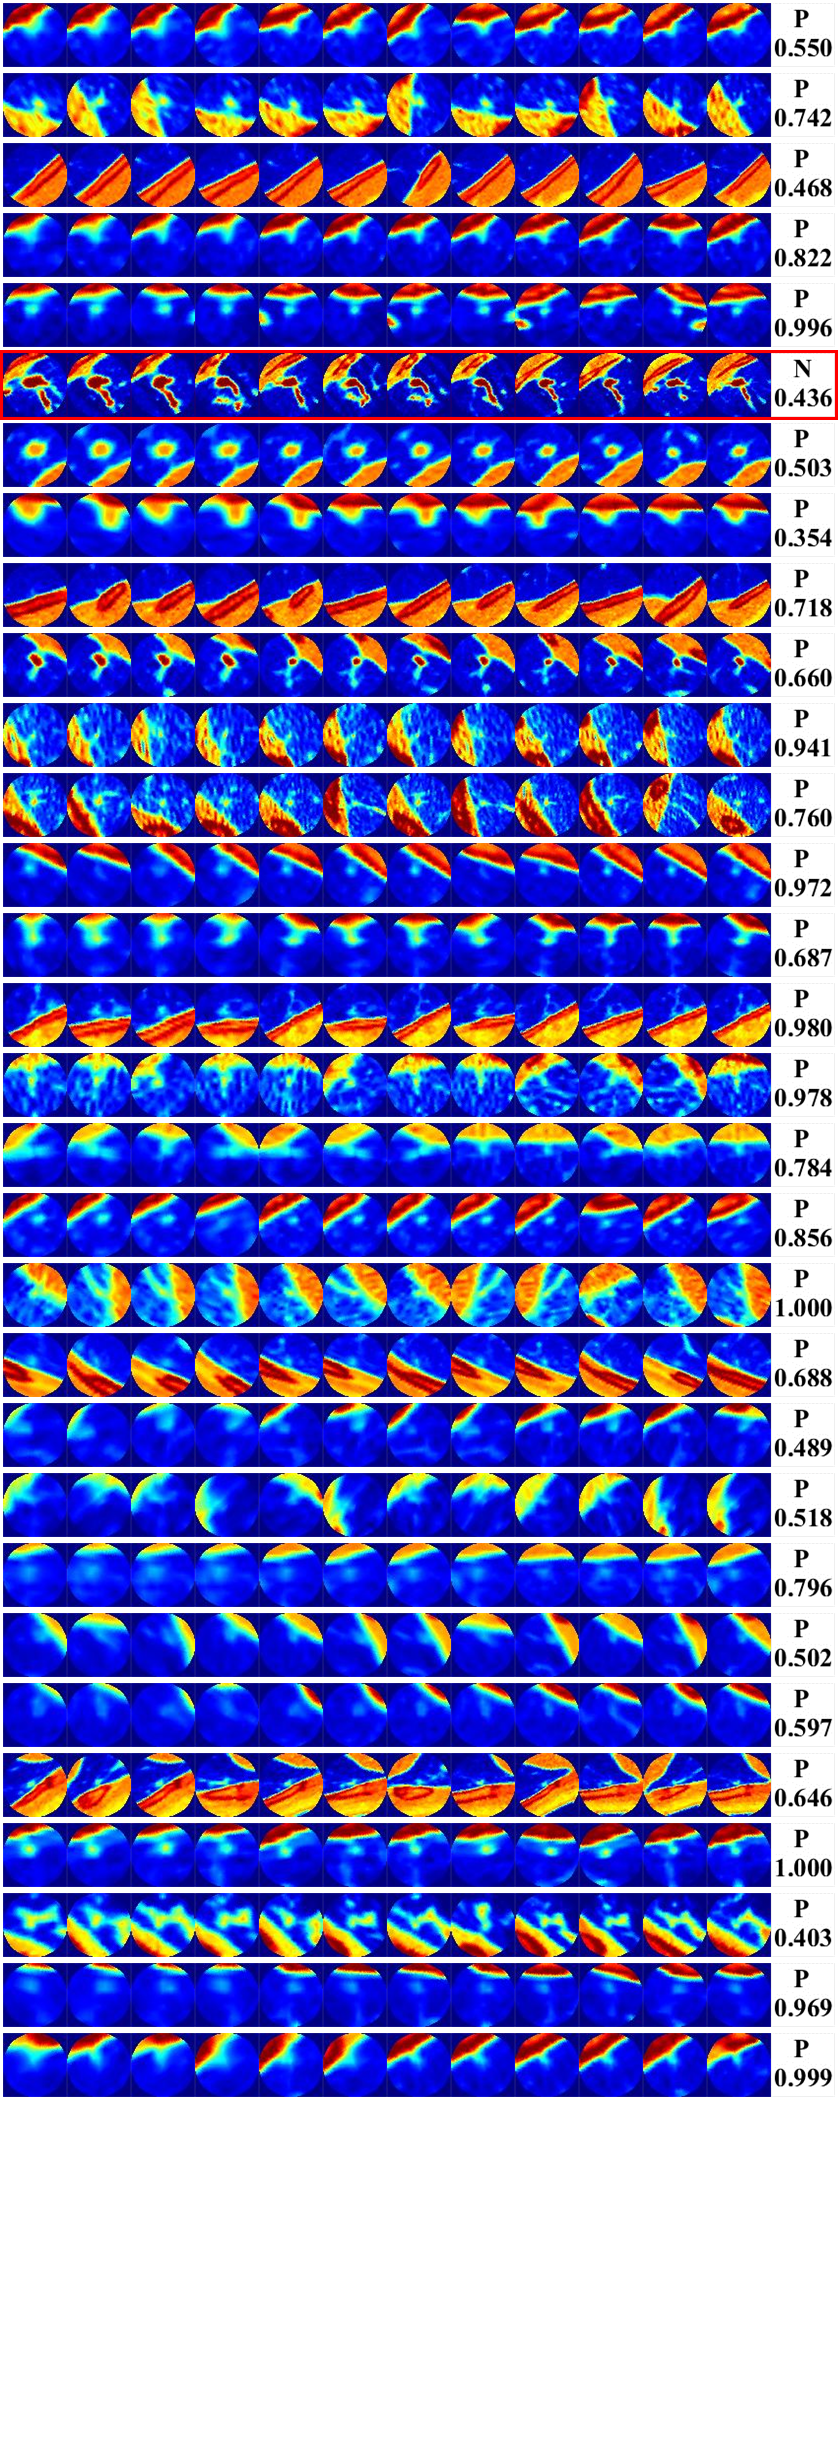
\includegraphics[width=0.45\columnwidth]{./images/elcap-msnodulecircles-tail1}
}
\end{figure}

\newpage
\subsection{Vascularized for \emph{ms-nodulecircles}}
\begin{figure}[H]
\centering
\subfigure{
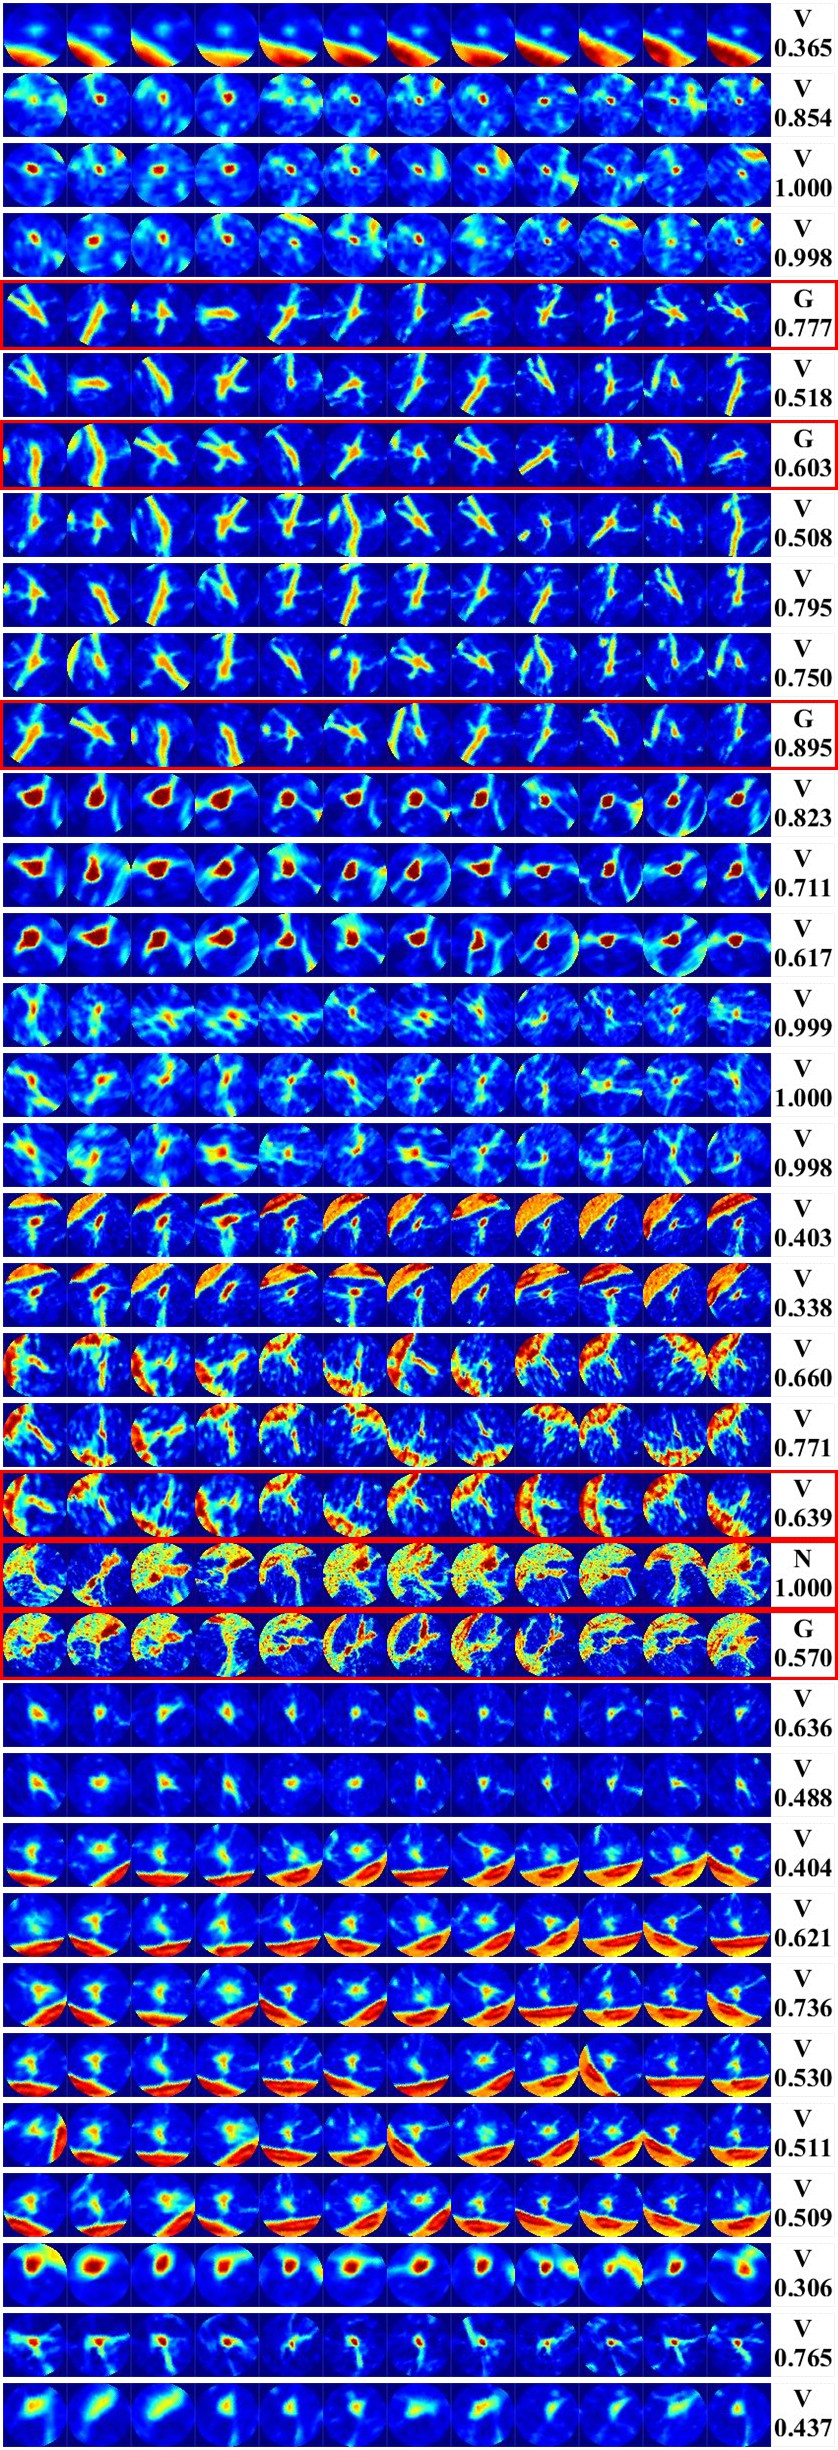
\includegraphics[width=0.45\columnwidth]{./images/elcap-msnodulecircles-vessel0}
}
\hspace{.1in}
\subfigure{
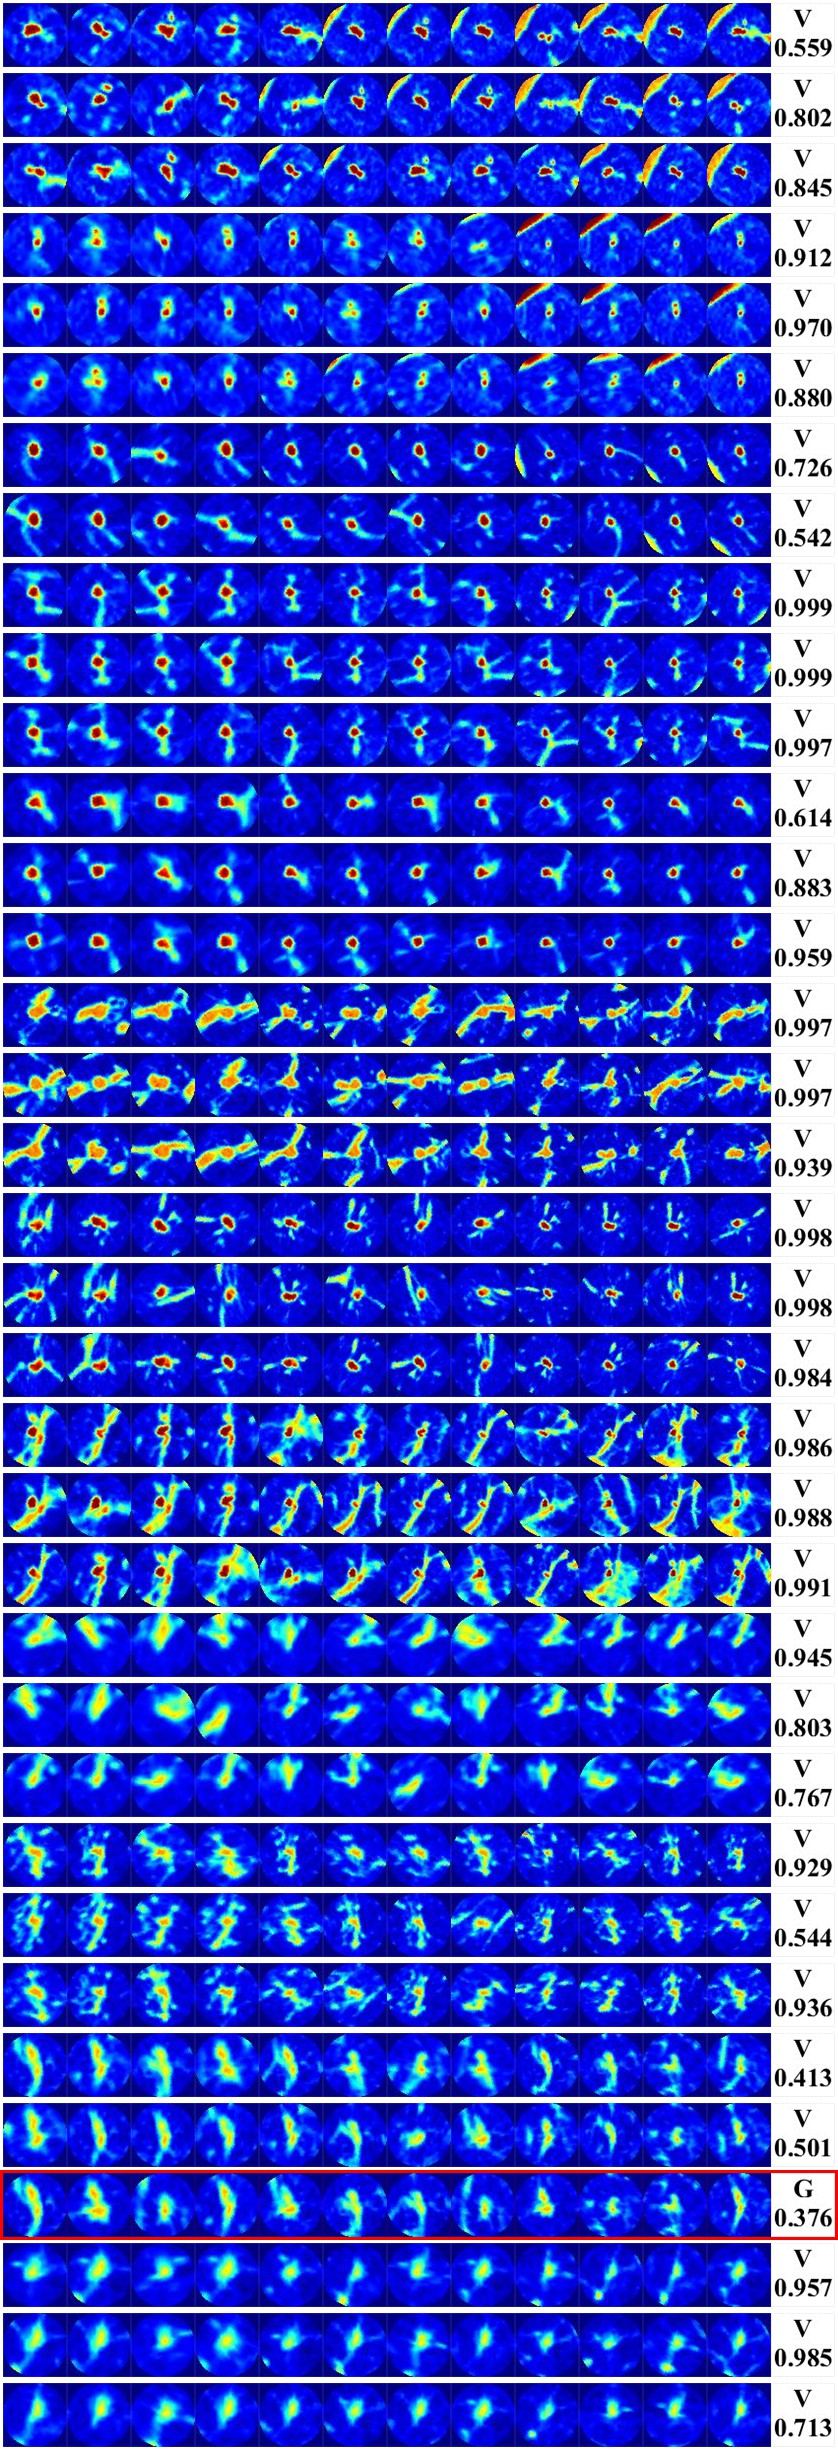
\includegraphics[width=0.45\columnwidth]{./images/elcap-msnodulecircles-vessel1}
}
\end{figure}
\newpage
\begin{figure}[H]
\centering
\subfigure{
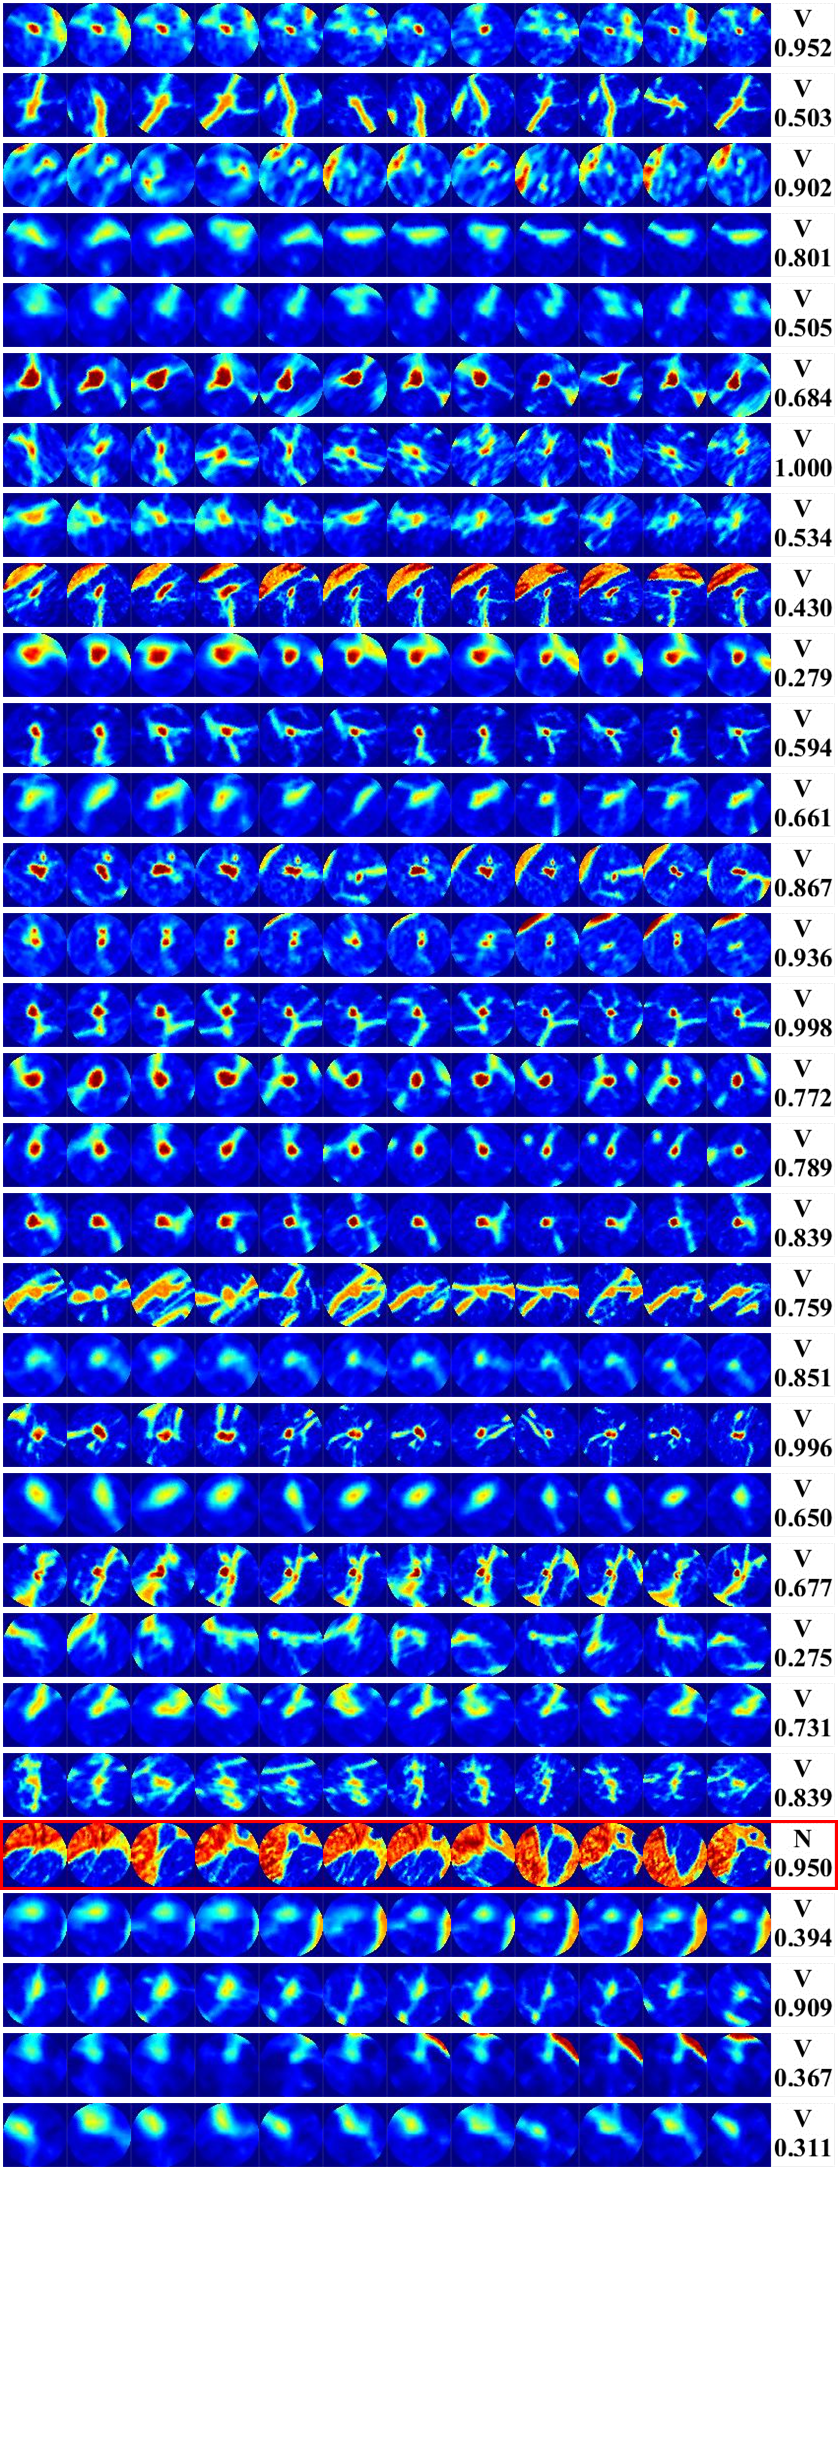
\includegraphics[width=0.45\columnwidth]{./images/elcap-msnodulecircles-vessel2}
}
\end{figure}

\newpage
\subsection{NON-NODULE for \emph{ms-nodulecircles}}
\begin{figure}[H]
\centering
\subfigure{
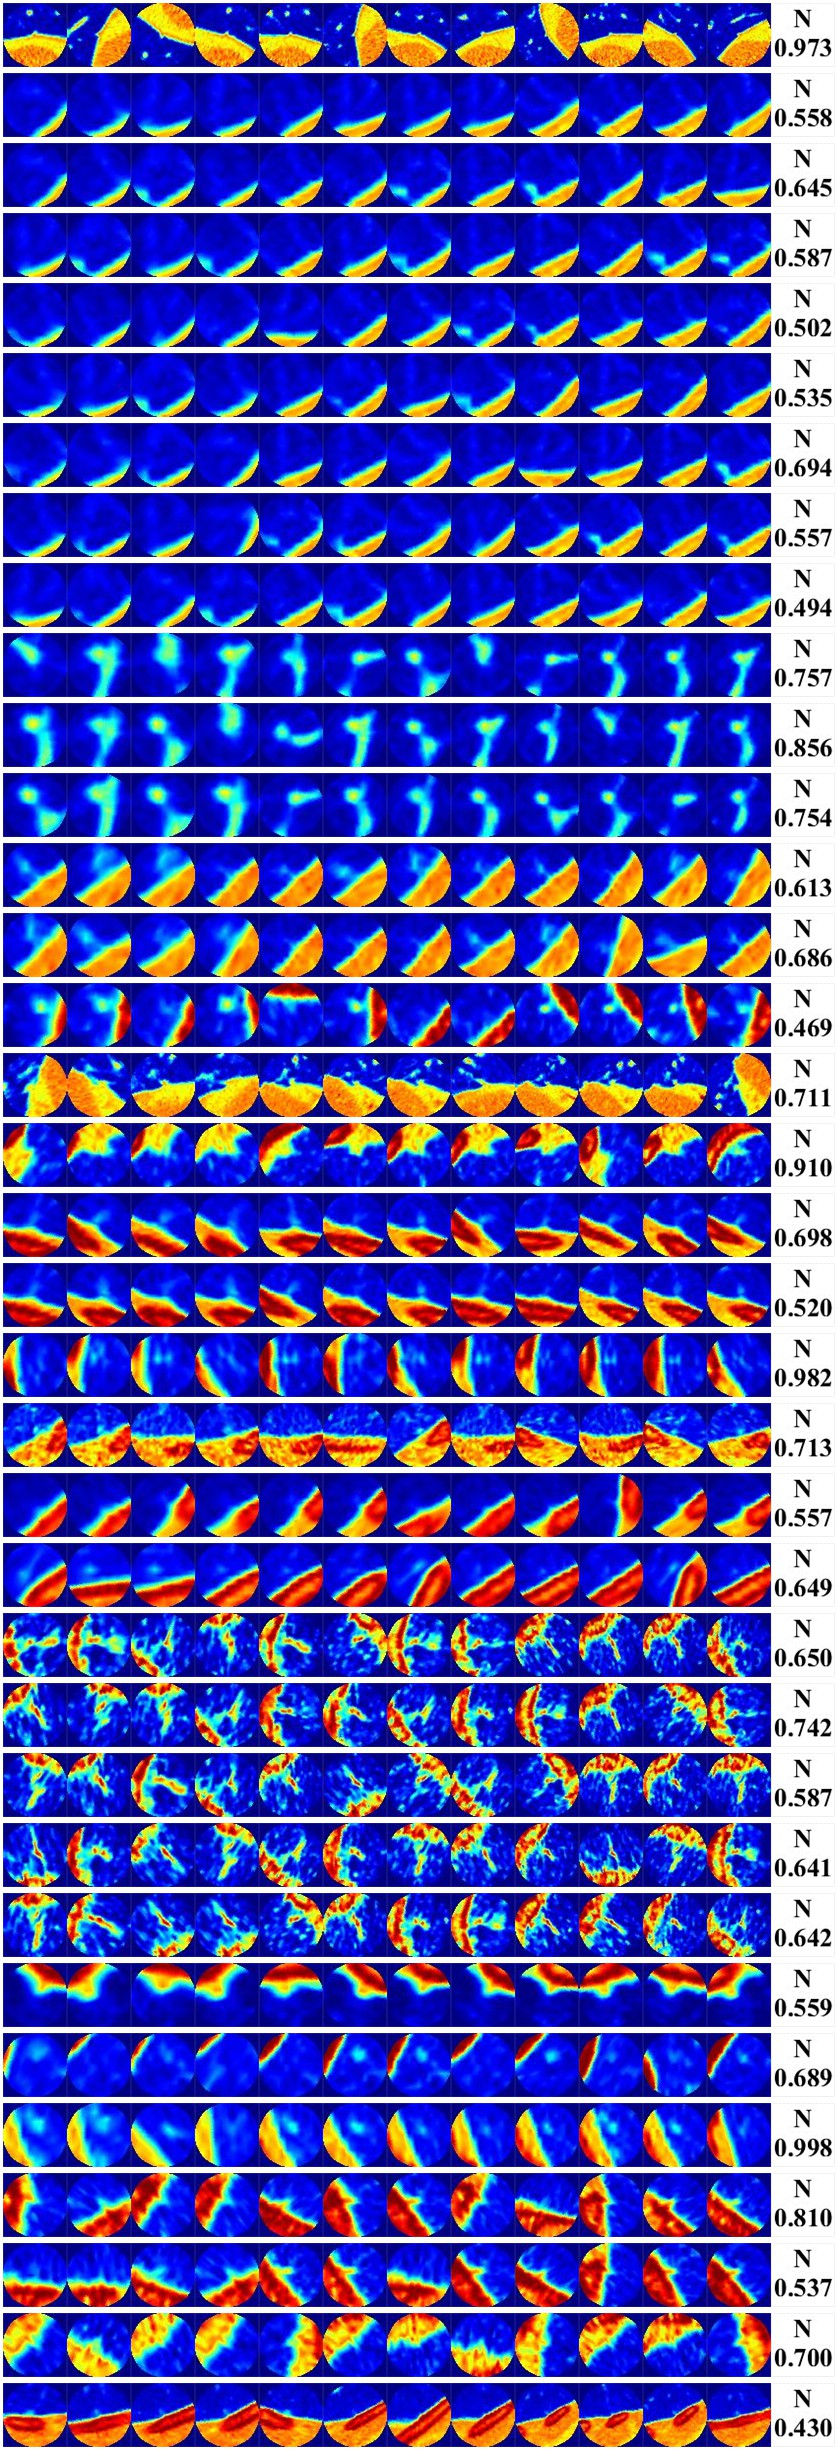
\includegraphics[width=0.45\columnwidth]{./images/elcap-msnodulecircles-nonnodule0}
}
\hspace{.1in}
\subfigure{
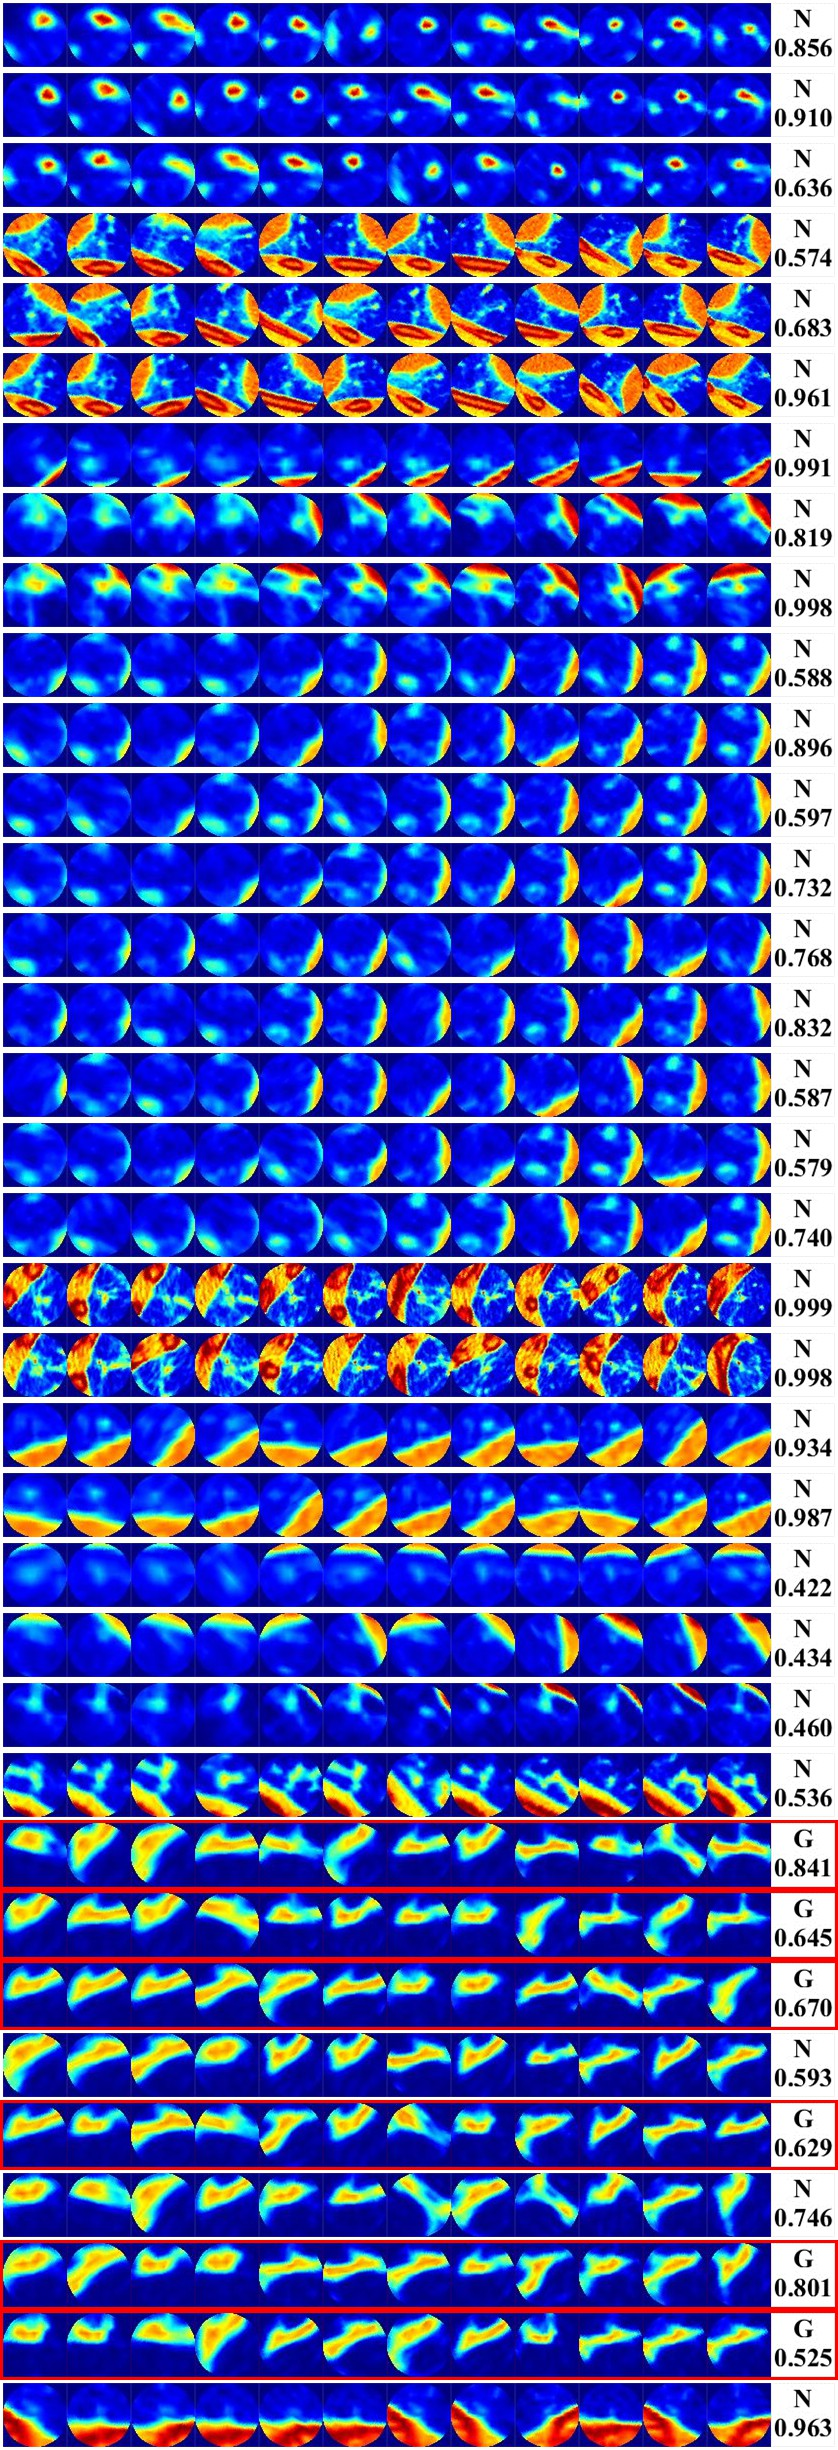
\includegraphics[width=0.45\columnwidth]{./images/elcap-msnodulecircles-nonnodule1}
}
\end{figure}
\newpage
\begin{figure}[H]
\centering
\subfigure{
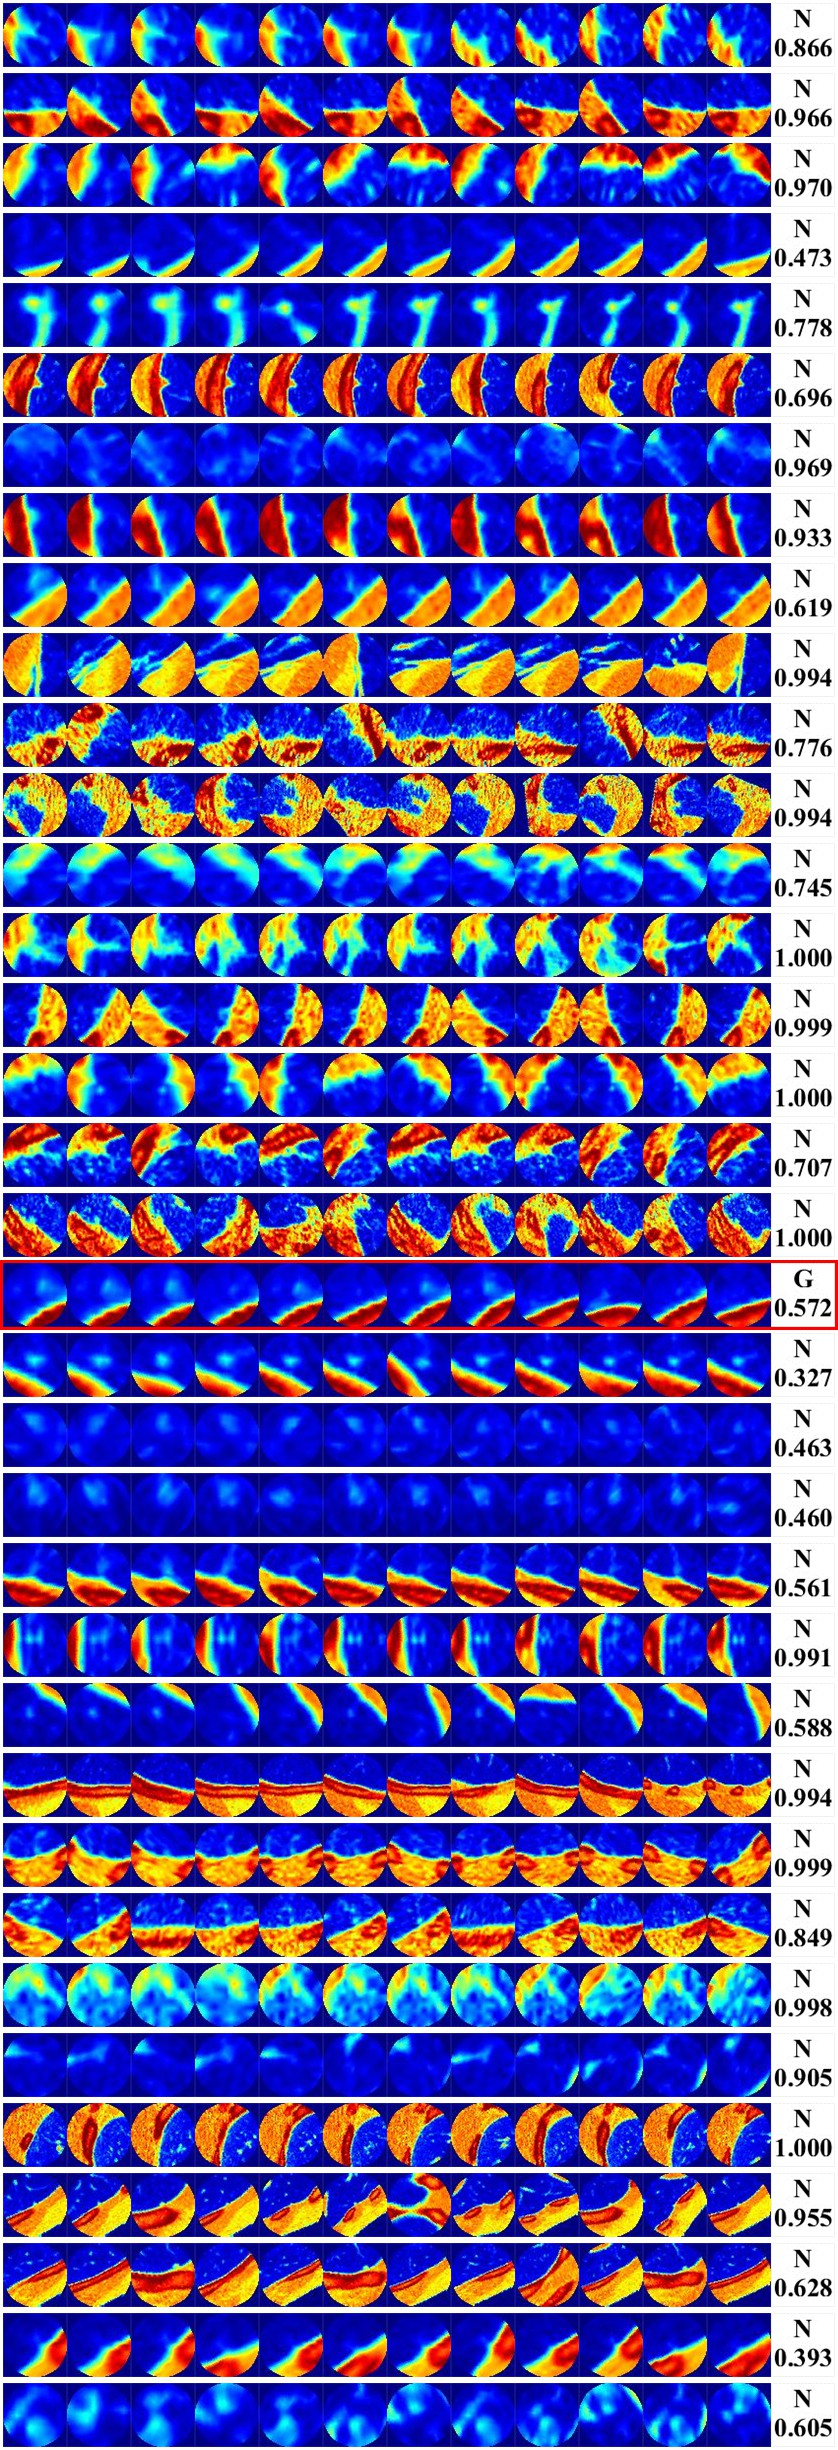
\includegraphics[width=0.45\columnwidth]{./images/elcap-msnodulecircles-nonnodule2}
}
\hspace{.1in}
\subfigure{
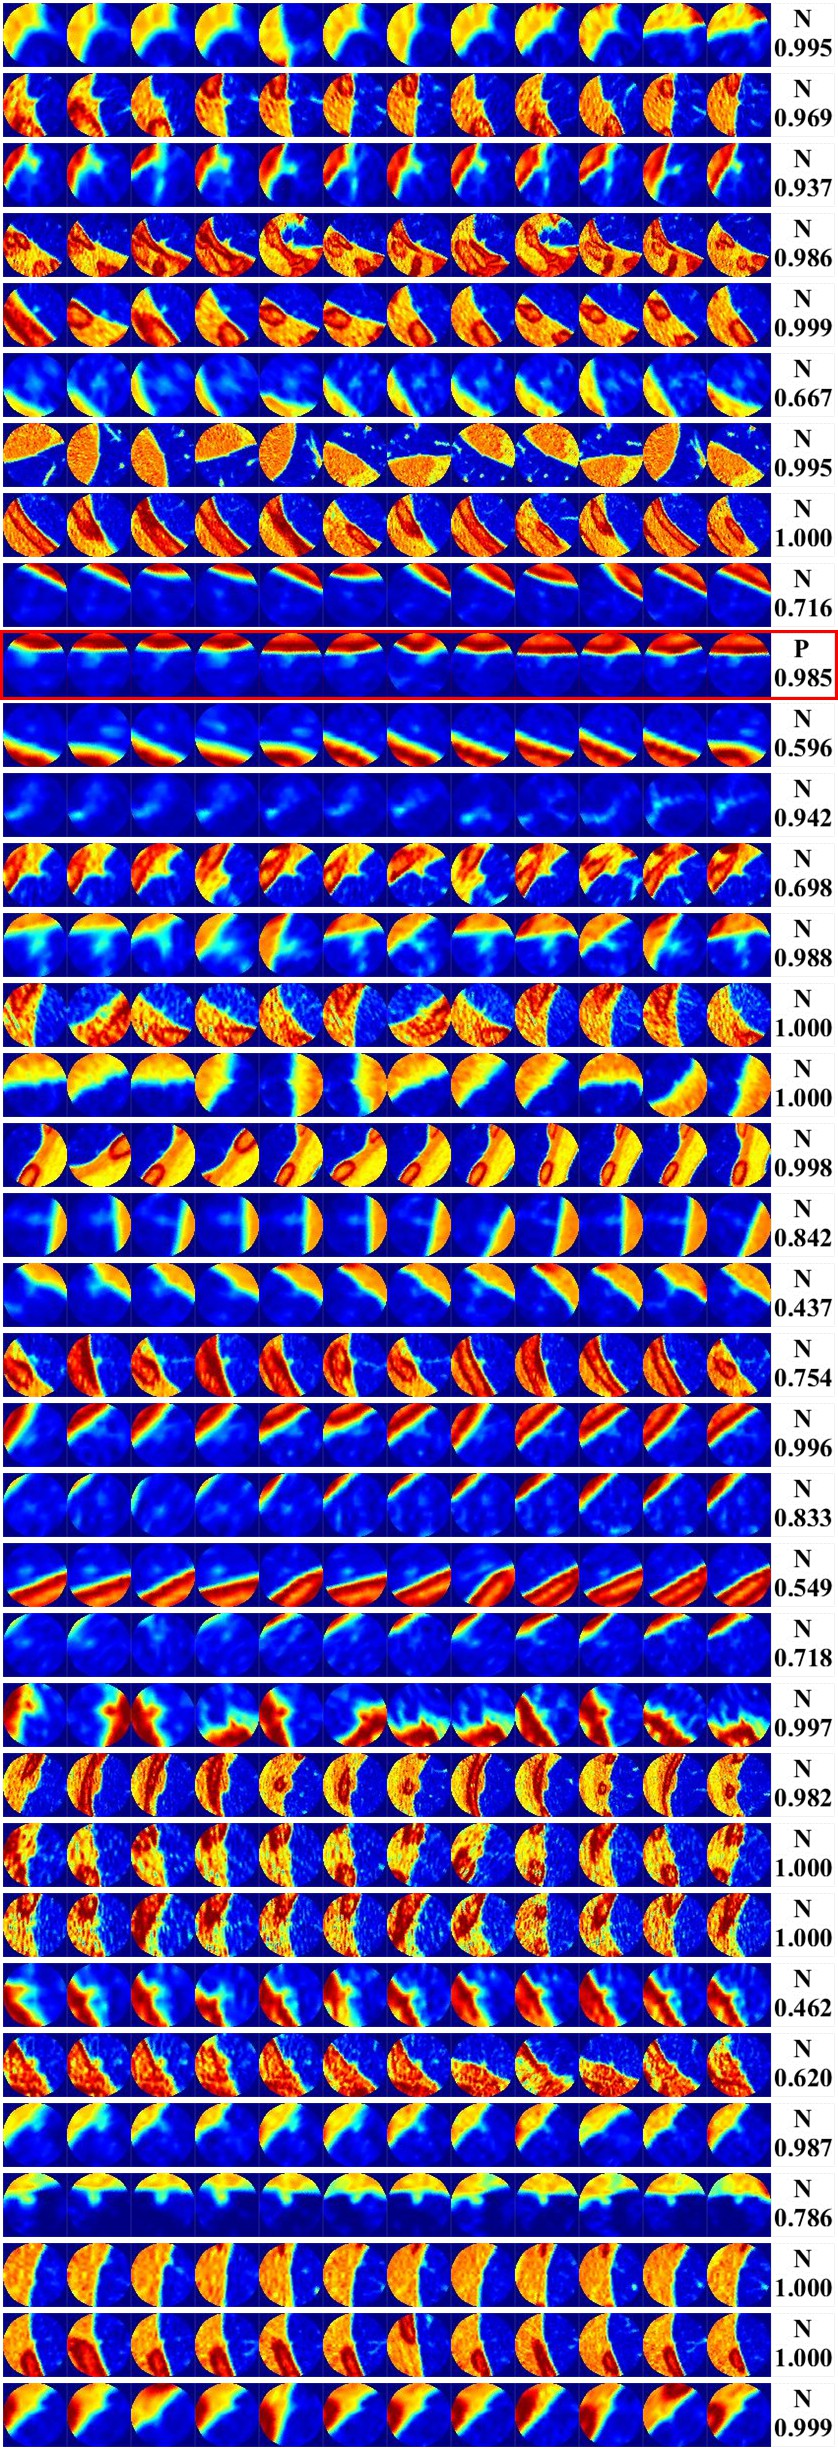
\includegraphics[width=0.45\columnwidth]{./images/elcap-msnodulecircles-nonnodule3}
}
\end{figure}
\newpage
\begin{figure}[H]
\centering
\subfigure{
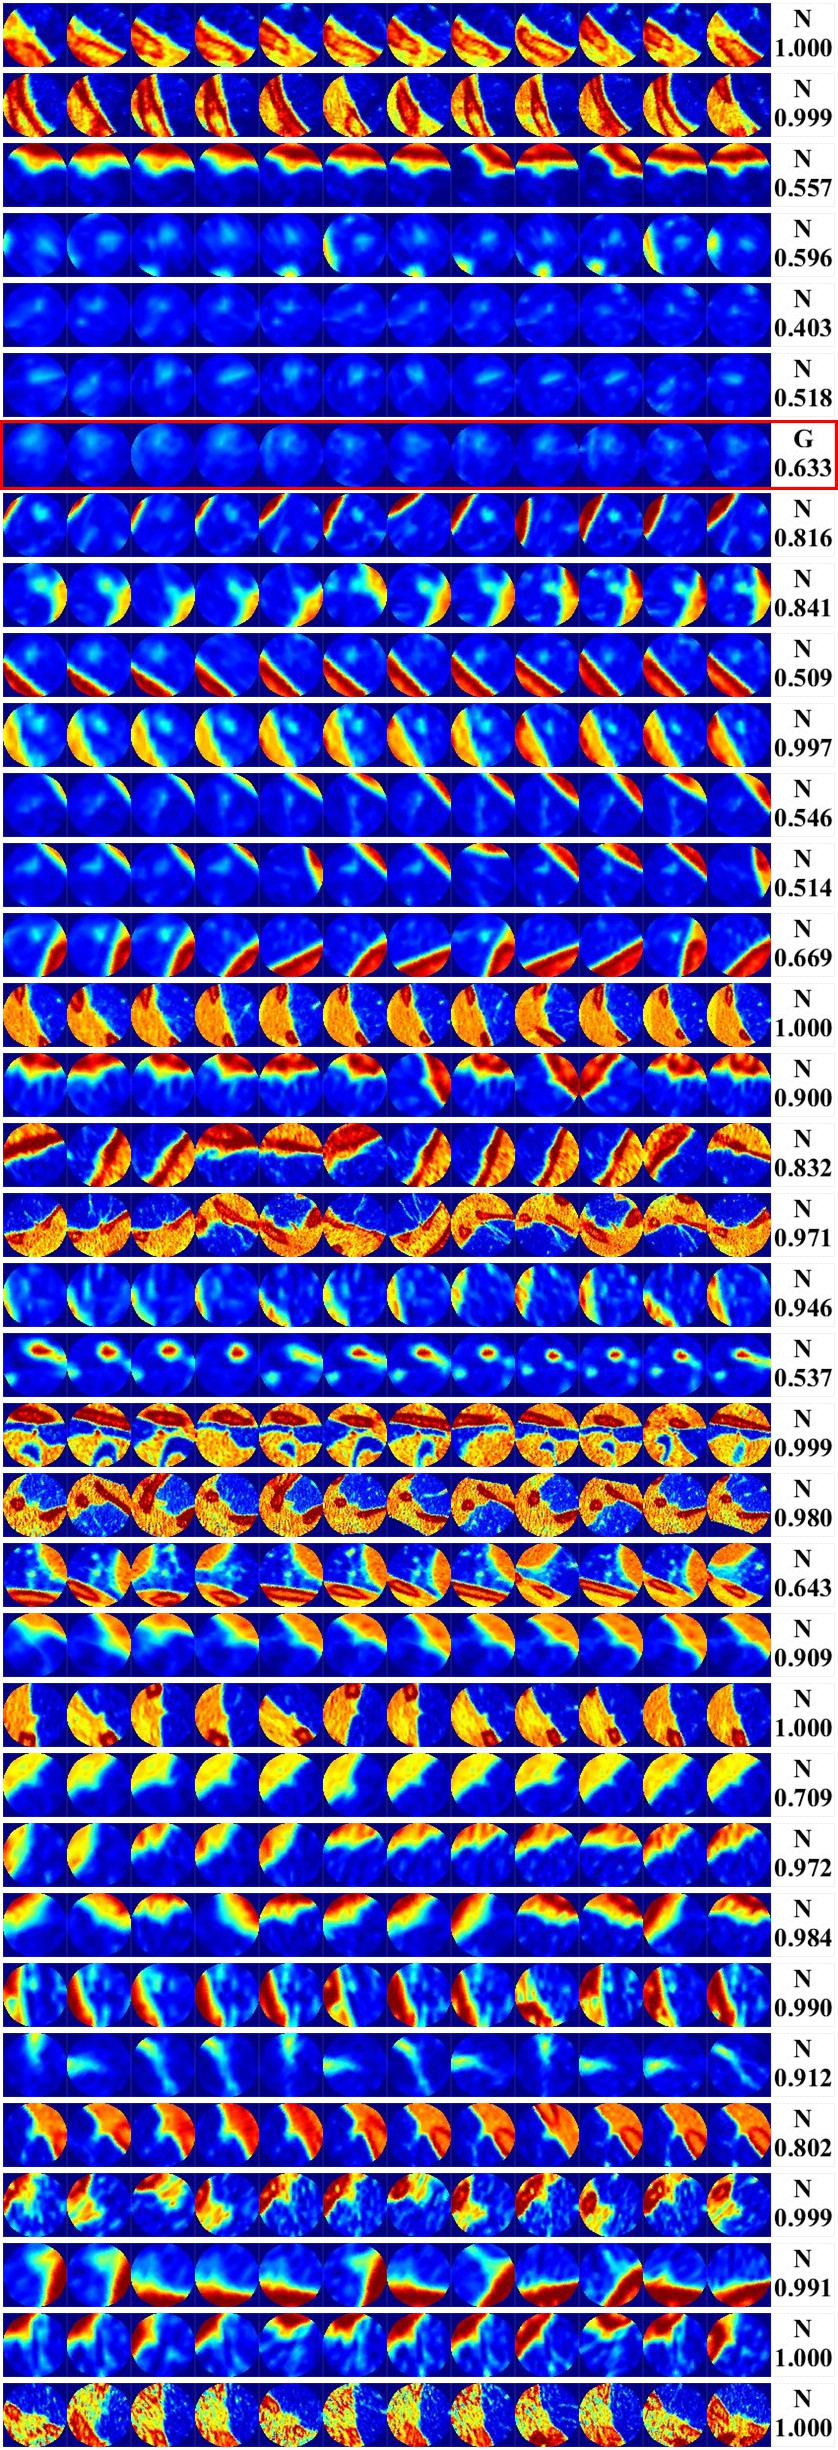
\includegraphics[width=0.45\columnwidth]{./images/elcap-msnodulecircles-nonnodule4}
}
\hspace{.1in}
\subfigure{
\includegraphics[width=0.45\columnwidth]{./images/elcap-msnodulecircles-nonnodule5}
}
\end{figure}
\newpage
\begin{figure}[H]
\centering
\subfigure{
\includegraphics[width=0.45\columnwidth]{./images/elcap-msnodulecircles-nonnodule6}
}
\hspace{.1in}
\subfigure{
\includegraphics[width=0.45\columnwidth]{./images/elcap-msnodulecircles-nonnodule7}
}
\end{figure}



\end{document}


